\documentclass{report}\usepackage[]{graphicx}\usepackage[usenames,dvipsnames]{color}
%% maxwidth is the original width if it is less than linewidth
%% otherwise use linewidth (to make sure the graphics do not exceed the margin)
\makeatletter
\def\maxwidth{ %
  \ifdim\Gin@nat@width>\linewidth
    \linewidth
  \else
    \Gin@nat@width
  \fi
}
\makeatother

\definecolor{fgcolor}{rgb}{0.251, 0.251, 0.251}
\newcommand{\hlnum}[1]{\textcolor[rgb]{0.816,0.125,0.439}{#1}}%
\newcommand{\hlstr}[1]{\textcolor[rgb]{0.251,0.627,0.251}{#1}}%
\newcommand{\hlcom}[1]{\textcolor[rgb]{0.502,0.502,0.502}{\textit{#1}}}%
\newcommand{\hlopt}[1]{\textcolor[rgb]{0,0,0}{#1}}%
\newcommand{\hlstd}[1]{\textcolor[rgb]{0.251,0.251,0.251}{#1}}%
\newcommand{\hlkwa}[1]{\textcolor[rgb]{0.125,0.125,0.941}{#1}}%
\newcommand{\hlkwb}[1]{\textcolor[rgb]{0,0,0}{#1}}%
\newcommand{\hlkwc}[1]{\textcolor[rgb]{0.251,0.251,0.251}{#1}}%
\newcommand{\hlkwd}[1]{\textcolor[rgb]{0.878,0.439,0.125}{#1}}%
\let\hlipl\hlkwb

\newenvironment{knitrout}{}{} % an empty environment to be redefined in TeX
\usepackage{alltt}
\usepackage{tikz}

\RequirePackage[]{Bioconductor2}
\AtBeginDocument{\bibliographystyle{unsrturl}}


\bioctitle[\Biocpkg{csaw} User's Guide]{\Biocpkg{csaw}: ChIP-seq analysis with windows \\ User's Guide}
%% also: \bioctitle{Title used for both header and title page}
%% or... \title{Title used for both header and title page}
\author[1,2]{Aaron T. L. Lun}
\author[1,3]{Gordon K. Smyth}
\affil[1]{The Walter and Eliza Hall Institute of Medical Research, Melbourne, Australia}
\affil[2]{Department of Medical Biology, The University of Melbourne, Melbourne, Australia}
\affil[3]{Department of Mathematics and Statistics, The University of Melbourne, Melbourne, Australia}

\usepackage{framed,color}
\newenvironment{combox}
{ \definecolor{shadecolor}{RGB}{255, 240, 240} \begin{shaded}\begin{center}\begin{minipage}[t]{0.95\textwidth} }
{ \end{minipage}\end{center}\end{shaded} \definecolor{shadecolor}{RGB}{240,240,240} }

\usepackage{bibentry}
\nobibliography*
\IfFileExists{upquote.sty}{\usepackage{upquote}}{}
\begin{document}
\maketitle
            
\begin{abstract}                            
This document contains instructions on how to use \Biocpkg{csaw} for differential binding analyses of ChIP-seq data with windows.
It covers read counting into windows, filtering for windows of interest, normalization of sample-specific biases, variance modelling and hypothesis testing,
summarization of windows into regions, and visualization and annotation of detected regions.

\vspace{0.05in}
\textit{First edition:} 15 August 2012 \\
\textit{Last revised:} 17 September 2017 \\
\textit{Last compiled:} 16 September 2017
\end{abstract}

\packageVersion{csaw 1.11.2}

\tableofcontents
\newpage



\chapter{Introduction}

\section{Scope}
This document gives an overview of the \Bioconductor{} package \Biocpkg{csaw} for detecting differential binding (DB) in ChIP-seq experiments.
\Biocpkg{csaw} uses sliding windows to identify significant changes in binding patterns for transcription factors (TFs) or histone marks across different biological conditions \cite{lun2016csaw}.
However, it can also be applied to any sequencing technique where reads represent coverage of enriched genomic regions.
The statistical methods described here are based upon those in the \Biocpkg{edgeR} package \cite{robinson2010}. 
Knowledge of \Biocpkg{edgeR} is useful but not a prerequesite for reading this guide.

\section{How to get help}
Most questions about \Biocpkg{csaw} should be answered by the documentation. 
Every function mentioned in this guide has its own help page. 
For example, a detailed description of the arguments and output of the \Rfunction{windowCounts} function can be obtained by typing \Rcode{?windowCounts} or \Rcode{help(windowCounts)} at the \R{} prompt. 
Further detail on the methods or the underlying theory can be found in the references at the bottom of each help page.

The authors of the package always appreciate receiving reports of bugs in the package functions or in the documentation. 
The same goes for well-considered suggestions for improvements. 
Other questions about how to use \Biocpkg{csaw} are best sent to the Bioconductor support site at \url{https://support.bioconductor.org}.
Please send requests for general assistance and advice to the support site, rather than to the individual authors. 
Users posting to the support site for the first time may find it helpful to read the posting guide at \url{http://www.bioconductor.org/help/support/posting-guide}.

\section{How to cite this package}
Most users of \Biocpkg{csaw} should cite the following in any publications:
\begin{quote}
\bibentry{lun2016csaw}
\end{quote}
Anyone who uses the Bioconductor \href{https://www.bioconductor.org/help/workflows/chipseqDB/}{workflow} to construct their analyses should also cite:
\begin{quote}
\bibentry{lun2015from}
\end{quote}
For people interested in combined $p$-values, their use in DB analyses was proposed in:
\begin{quote}
\bibentry{lun2014}
\end{quote}
The DB analyses shown here use methods from the \Biocpkg{edgeR} package, which has its own citation recommendations.
See the appropriate section of the \Biocpkg{edgeR} user's guide for more details.

\section{Quick start}
A typical ChIP-seq analysis in \Biocpkg{csaw} would look something like that described below. 
This assumes that a vector of file paths to sorted and indexed BAM files is provided in \Robject{bam.files} and a design matrix in supplied in \Robject{design}.
The code is split across several steps:



\begin{enumerate}
\item Loading in data from BAM files.
\begin{knitrout}
\definecolor{shadecolor}{rgb}{0.941, 0.941, 0.941}\color{fgcolor}\begin{kframe}
\begin{alltt}
\hlkwd{require}\hlstd{(csaw)}
\hlstd{param} \hlkwb{<-} \hlkwd{readParam}\hlstd{(}\hlkwc{minq}\hlstd{=}\hlnum{50}\hlstd{)}
\hlstd{data} \hlkwb{<-} \hlkwd{windowCounts}\hlstd{(bam.files,} \hlkwc{ext}\hlstd{=}\hlnum{110}\hlstd{,} \hlkwc{width}\hlstd{=}\hlnum{10}\hlstd{,} \hlkwc{param}\hlstd{=param)}
\end{alltt}
\end{kframe}
\end{knitrout}
\item Filtering out uninteresting regions.
\begin{knitrout}
\definecolor{shadecolor}{rgb}{0.941, 0.941, 0.941}\color{fgcolor}\begin{kframe}
\begin{alltt}
\hlkwd{require}\hlstd{(edgeR)}
\hlstd{keep} \hlkwb{<-} \hlkwd{aveLogCPM}\hlstd{(}\hlkwd{asDGEList}\hlstd{(data))} \hlopt{>= -}\hlnum{1}
\hlstd{data} \hlkwb{<-} \hlstd{data[keep,]}
\end{alltt}
\end{kframe}
\end{knitrout}
\item Calculating normalization factors.
\begin{knitrout}
\definecolor{shadecolor}{rgb}{0.941, 0.941, 0.941}\color{fgcolor}\begin{kframe}
\begin{alltt}
\hlstd{binned} \hlkwb{<-} \hlkwd{windowCounts}\hlstd{(bam.files,} \hlkwc{bin}\hlstd{=}\hlnum{TRUE}\hlstd{,} \hlkwc{width}\hlstd{=}\hlnum{10000}\hlstd{,} \hlkwc{param}\hlstd{=param)}
\hlstd{data} \hlkwb{<-} \hlkwd{normOffsets}\hlstd{(binned,} \hlkwc{se.out}\hlstd{=data)}
\end{alltt}
\end{kframe}
\end{knitrout}
\item Identifying DB windows.
\begin{knitrout}
\definecolor{shadecolor}{rgb}{0.941, 0.941, 0.941}\color{fgcolor}\begin{kframe}
\begin{alltt}
\hlstd{y} \hlkwb{<-} \hlkwd{asDGEList}\hlstd{(data)}
\hlstd{y} \hlkwb{<-} \hlkwd{estimateDisp}\hlstd{(y, design)}
\hlstd{fit} \hlkwb{<-} \hlkwd{glmQLFit}\hlstd{(y, design,} \hlkwc{robust}\hlstd{=}\hlnum{TRUE}\hlstd{)}
\hlstd{results} \hlkwb{<-} \hlkwd{glmQLFTest}\hlstd{(fit)}
\end{alltt}
\end{kframe}
\end{knitrout}
\item Correcting for multiple testing.
\begin{knitrout}
\definecolor{shadecolor}{rgb}{0.941, 0.941, 0.941}\color{fgcolor}\begin{kframe}
\begin{alltt}
\hlstd{merged} \hlkwb{<-} \hlkwd{mergeWindows}\hlstd{(}\hlkwd{rowRanges}\hlstd{(data),} \hlkwc{tol}\hlstd{=}\hlnum{1000L}\hlstd{)}
\hlstd{tabcom} \hlkwb{<-} \hlkwd{combineTests}\hlstd{(merged}\hlopt{$}\hlstd{id, results}\hlopt{$}\hlstd{table)}
\end{alltt}
\end{kframe}
\end{knitrout}
\end{enumerate}

In this guide, the behavior of each step will be demonstrated with some publicly available data.
The dataset below focuses on changes in the binding profile of the NFYA protein between embryonic stem cells and terminal neurons \cite{tiwari2012}. 
This will be used as a case study for most of the code examples throughout the guide.

\begin{knitrout}
\definecolor{shadecolor}{rgb}{0.941, 0.941, 0.941}\color{fgcolor}\begin{kframe}
\begin{alltt}
\hlstd{bam.files} \hlkwb{<-} \hlkwd{c}\hlstd{(}\hlstr{"es_1.bam"}\hlstd{,} \hlstr{"es_2.bam"}\hlstd{,} \hlstr{"tn_1.bam"}\hlstd{,} \hlstr{"tn_2.bam"}\hlstd{)}
\hlstd{design} \hlkwb{<-} \hlkwd{model.matrix}\hlstd{(}\hlopt{~}\hlkwd{factor}\hlstd{(}\hlkwd{c}\hlstd{(}\hlstr{'es'}\hlstd{,} \hlstr{'es'}\hlstd{,} \hlstr{'tn'}\hlstd{,} \hlstr{'tn'}\hlstd{)))}
\hlkwd{colnames}\hlstd{(design)} \hlkwb{<-} \hlkwd{c}\hlstd{(}\hlstr{"intercept"}\hlstd{,} \hlstr{"cell.type"}\hlstd{)}
\end{alltt}
\end{kframe}
\end{knitrout}
\label{data:main}

A comprehensive listing of the datasets used in this guide is provided in Section~\ref{sec:dataset}, along with instructions on how to obtain and process them for entry into the \Biocpkg{csaw} pipeline.

%%%%%%%%%%%%%%%%%%%%%%%%%%%%%%%%%%%%%%%%%%%%%%%%%%%%%%%%%%%%%%%%%%%%%%%%%%%%%%%%%%%%%%%%%%%%%%%%%%%
%%%%%%%%%%%%%%%%%%%%%%%%%%%%%%%%%%%%%%%%%%%%%%%%%%%%%%%%%%%%%%%%%%%%%%%%%%%%%%%%%%%%%%%%%%%%%%%%%%%
%%%%%%%%%%%%%%%%%%%%%%%%%%%%%%%%%%%%%%%%%%%%%%%%%%%%%%%%%%%%%%%%%%%%%%%%%%%%%%%%%%%%%%%%%%%%%%%%%%%

\chapter{Converting reads to counts}
\label{chap:count}
\begin{combox}
Hello, reader.
A little box like this will be present at the start of each chapter.
The idea is to list the objects from previous chapters that are needed to run the code in the current chapter.
Hopefully, it'll provide a nice segue between chapters for tired eyes.
At this point, all we need are the \Robject{bam.files} that we defined in the introduction above.
\end{combox}

\section{Types of input data}
Sorted and indexed BAM (i.e., binary SAM) files \cite{li2009} are required as input into the read counting functions in \Biocpkg{csaw}. 
Sorting should be performed on the genomic coordinates of the mapped reads.
Each read should only have one alignment in the file, i.e., secondary alignments should not be present.

For a given BAM file named \file{xxx.bam}, the corresponding index file should be named as \file{xxx.bam.bai} in the same directory. 
The sensibility of the supplied index is not checked prior to counting. 
A common mistake is to replace or update the BAM file without updating the index. 
This will cause \Biocpkg{csaw} to return incorrect results when it attempts to load alignments from the new BAM file.

\section{Counting reads into windows}

\subsection{Overview}
The \Rfunction{windowCounts} function uses a sliding window approach to count fragments for a set of libraries. 
For single-end data, the fragment corresponding to a read is imputed by directionally extending each read to the average fragment length. 
We define a window as a fixed-width genomic interval, and we count the number of fragments overlapping that window in each library.
This is repeated after sliding the window along the genome to a new position. 
A count is then obtained for each window in each library, thus quantifying protein binding intensity across the genome.

\begin{knitrout}
\definecolor{shadecolor}{rgb}{0.941, 0.941, 0.941}\color{fgcolor}\begin{kframe}
\begin{alltt}
\hlstd{frag.len} \hlkwb{<-} \hlnum{110}
\hlstd{win.width} \hlkwb{<-} \hlnum{10}
\hlstd{param} \hlkwb{<-} \hlkwd{readParam}\hlstd{(}\hlkwc{minq}\hlstd{=}\hlnum{50}\hlstd{)}
\hlstd{data} \hlkwb{<-} \hlkwd{windowCounts}\hlstd{(bam.files,} \hlkwc{ext}\hlstd{=frag.len,} \hlkwc{width}\hlstd{=win.width,} \hlkwc{param}\hlstd{=param)}
\end{alltt}
\end{kframe}
\end{knitrout}

The function returns a \Rclass{RangedSummarizedExperiment} object where the matrix of counts is stored as the first entry in the \Rcode{assays} slot.
Each row corresponds to a genomic window while each column corresponds to a library.
The coordinates of each window are stored in the \Rcode{rowRanges} slot.
The total number of reads in each library (also referred to as the library size) is stored as \Rcode{totals} in the \Rcode{colData} slot.

\begin{knitrout}
\definecolor{shadecolor}{rgb}{0.941, 0.941, 0.941}\color{fgcolor}\begin{kframe}
\begin{alltt}
\hlkwd{head}\hlstd{(}\hlkwd{assay}\hlstd{(data))}
\end{alltt}
\begin{verbatim}
##      [,1] [,2] [,3] [,4]
## [1,]    3    3    1    3
## [2,]    5    6    1    3
## [3,]    7    5    0    0
## [4,]    4    7    0    0
## [5,]    3    7    0    0
## [6,]    1    2    2    6
\end{verbatim}
\begin{alltt}
\hlkwd{head}\hlstd{(}\hlkwd{rowRanges}\hlstd{(data))}
\end{alltt}
\begin{verbatim}
## GRanges object with 6 ranges and 0 metadata columns:
##       seqnames             ranges strand
##          <Rle>          <IRanges>  <Rle>
##   [1]     chr1 [3003701, 3003710]      *
##   [2]     chr1 [3003751, 3003760]      *
##   [3]     chr1 [3003801, 3003810]      *
##   [4]     chr1 [3004001, 3004010]      *
##   [5]     chr1 [3004051, 3004060]      *
##   [6]     chr1 [3007551, 3007560]      *
##   -------
##   seqinfo: 66 sequences from an unspecified genome
\end{verbatim}
\begin{alltt}
\hlstd{data}\hlopt{$}\hlstd{totals}
\end{alltt}
\begin{verbatim}
## [1] 17196528 20040530 23118590 22075821
\end{verbatim}
\end{kframe}
\end{knitrout}

For single-end data, we estimate the average fragment length from a cross-correlation plot (see Section~\ref{sec:ccf}) for use as \Rcode{ext}.
Alternatively, the length can be estimated from diagnostics during ChIP or library preparation, e.g., post-fragmentation gel electrophoresis images. 
Typical values range from 100 to 300 bp, depending on the efficiency of sonication and the use of size selection steps in library preparation.

\begin{center}
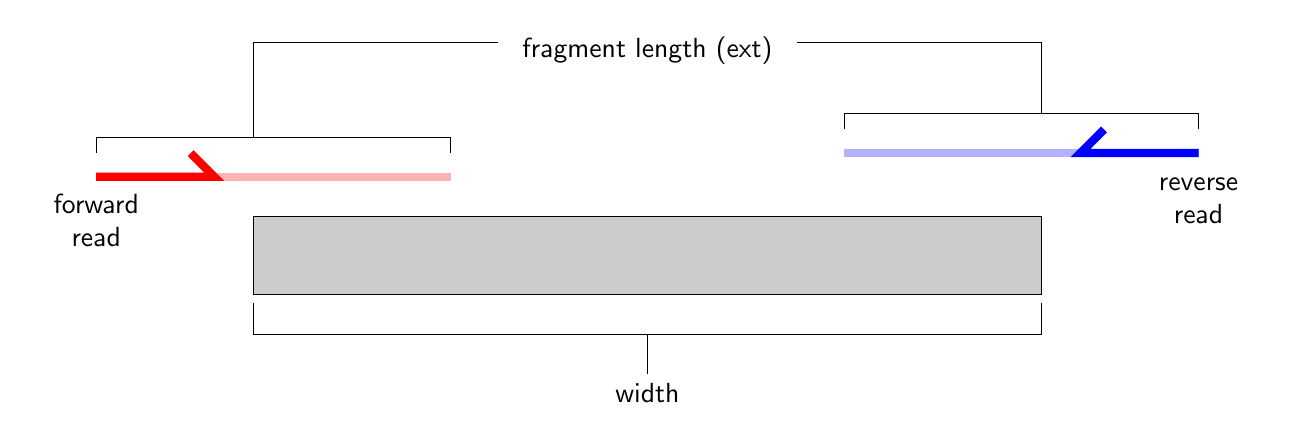
\begin{tikzpicture}[font=\sffamily]
% Filling the left region.
\filldraw[fill=black!20] (0,0) rectangle (10,1);
\draw (0,-0.1)--(0,-0.5)--(10,-0.5)--(10,-0.1);
\draw (5,-0.5)--(5,-1);
\node[below] at (5, -1) {width};

% Adding left read.
\draw[line width=3pt,color=red!30] (-2,1.5)--(2.5,1.5);
\draw[line width=3pt,color=red] (-2,1.5)--(-0.5,1.5)--(-0.8,1.8);
\draw (-2,1.8)--(-2,2)--(2.5,2)--(2.5,1.8);
\node[below] at (-2,1.45) {\begin{tabular}{c} forward \\ read \end{tabular}};

% Adding the right read
\draw[line width=3pt,color=blue!30] (12,1.8)--(7.5,1.8);
\draw[line width=3pt,color=blue] (12,1.8)--(10.5,1.8)--(10.8,2.1);
\draw (12,2.1)--(12,2.3)--(7.5,2.3)--(7.5,2.1);
\node[below] at (12,1.75) {\begin{tabular}{c} reverse \\ read \end{tabular}};

\draw (0,2)--(0,3.2)--(3.1,3.2);
\draw (10,2.3)--(10,3.2)--(6.9,3.2);
\node[above] at (5,2.8) {fragment length (ext)};
\end{tikzpicture}
\end{center}

The \Rcode{width} argument defines the window size, which we interpret as the width of the binding site for the target protein.
This is user-specified and has important implications for the power and resolution of a DB analysis, which are discussed in Section~\ref{sec:windowsize}.
For TF analyses with small windows, the choice of spacing interval will also be affected by the choice of window size -- see Section~\ref{sec:efficiency} for more details.

\subsection{Filtering out low-quality reads}
Read extraction from the BAM files is controlled with the \Rcode{param} argument in \Rfunction{windowCounts}.
This takes a \Rclass{readParam} object that specifies a number of extraction parameters.
The idea is to define the \Rclass{readParam} object once in the entire analysis pipeline, which is then reused for all relevant functions.
This ensures that read loading is consistent throughout the analysis.

\begin{knitrout}
\definecolor{shadecolor}{rgb}{0.941, 0.941, 0.941}\color{fgcolor}\begin{kframe}
\begin{alltt}
\hlstd{param}
\end{alltt}
\begin{verbatim}
##     Extracting reads in single-end mode
##     Duplicate removal is turned off 
##     Minimum allowed mapping score is 50 
##     Reads are extracted from both strands
##     No restrictions are placed on read extraction
##     No regions are specified to discard reads
##     Using SerialParam with 1 worker
\end{verbatim}
\end{kframe}
\end{knitrout}

In the example above, reads are filtered out based on the minimum mapping score with the \Rcode{minq} argument. 
Low mapping scores are indicative of incorrectly and/or non-uniquely aligned sequences. 
Removal of these reads is highly recommended as it will ensure that only the reliable alignments are supplied to \Biocpkg{csaw}.
The exact value of the threshold depends on the range of scores provided by the aligner. 
The \software{subread} program \cite{liao2013} was used to align the reads in this dataset, so a value of 50 might be appropriate.

Reads mapping to the same genomic position can be marked as putative PCR duplicates using software like the \software{MarkDuplicates} program from the \software{Picard} suite.
Marked reads in the BAM file can be ignored during counting by setting \Rcode{dedup=TRUE} in the \Rclass{readParam} object. 
This reduces the variability caused by inconsistent amplification between replicates, and avoid spurious duplicate-driven DB between groups. 
An example of counting with duplicate removal is shown below, where fewer reads are used from each library relative to \Rcode{data\$totals}.

\begin{knitrout}
\definecolor{shadecolor}{rgb}{0.941, 0.941, 0.941}\color{fgcolor}\begin{kframe}
\begin{alltt}
\hlstd{dedup.param} \hlkwb{<-} \hlkwd{readParam}\hlstd{(}\hlkwc{minq}\hlstd{=}\hlnum{50}\hlstd{,} \hlkwc{dedup}\hlstd{=}\hlnum{TRUE}\hlstd{)}
\hlstd{demo} \hlkwb{<-} \hlkwd{windowCounts}\hlstd{(bam.files,} \hlkwc{ext}\hlstd{=frag.len,} \hlkwc{width}\hlstd{=win.width,}
                     \hlkwc{param}\hlstd{=dedup.param)}
\hlstd{demo}\hlopt{$}\hlstd{totals}
\end{alltt}
\begin{verbatim}
## [1] 13925800 13826445 16342981 18905912
\end{verbatim}
\end{kframe}
\end{knitrout}

Duplicate removal is generally not recommended for routine DB analyses. 
This is because it caps the number of reads at each position, reducing DB detection power in high-abundance regions. 
Spurious differences may also be introduced when the same upper bound is applied to libraries of varying size. 
However, it may be unavoidable in some cases, e.g., involving libraries generated from low quantities of DNA.
Duplicate removal is also acceptable for paired-end data, as exact overlaps for both paired reads are required to define duplicates.
This greatly reduces the probability of incorrectly discarding read pairs from non-duplicate DNA fragments
(assuming that a pair-aware method was used during duplicate marking).

\subsection{Avoiding problematic genomic regions}
Read extraction and counting can be restricted to particular chromosomes by specifying the names of the chromosomes of interest in \Rcode{restrict}. 
This avoids the need to count reads on unassigned contigs or uninteresting chromosomes, e.g., the mitochondrial genome for ChIP-seq studies targeting nuclear factors. 
Alternatively, it allows \Rfunction{windowCounts} to work on huge datasets or in limited memory by analyzing only one chromosome at a time.

\begin{knitrout}
\definecolor{shadecolor}{rgb}{0.941, 0.941, 0.941}\color{fgcolor}\begin{kframe}
\begin{alltt}
\hlstd{restrict.param} \hlkwb{<-} \hlkwd{readParam}\hlstd{(}\hlkwc{restrict}\hlstd{=}\hlkwd{c}\hlstd{(}\hlstr{"chr1"}\hlstd{,} \hlstr{"chr10"}\hlstd{,} \hlstr{"chrX"}\hlstd{))}
\end{alltt}
\end{kframe}
\end{knitrout}

Reads lying in certain regions can also be removed by specifying the coordinates of those regions in \Rcode{discard}. 
This is intended to remove reads that are wholly aligned within known repeat regions but were not removed by the \Rcode{minq} filter. 
Repeats are problematic as changes in repeat copy number or accessibility between conditions can lead to spurious DB. 
Removal of reads within repeat regions can avoid detection of these irrelevant differences. 

\begin{knitrout}
\definecolor{shadecolor}{rgb}{0.941, 0.941, 0.941}\color{fgcolor}\begin{kframe}
\begin{alltt}
\hlstd{repeats} \hlkwb{<-} \hlkwd{GRanges}\hlstd{(}\hlstr{"chr1"}\hlstd{,} \hlkwd{IRanges}\hlstd{(}\hlnum{3000001}\hlstd{,} \hlnum{3041000}\hlstd{))} \hlcom{# telomere}
\hlstd{discard.param} \hlkwb{<-} \hlkwd{readParam}\hlstd{(}\hlkwc{discard}\hlstd{=repeats)}
\end{alltt}
\end{kframe}
\end{knitrout}

Coordinates of annotated repeats can be obtained from several different sources.
A curated blacklist of problematic regions is available from the ENCODE project \cite{dunham2012}, and can be obtained at \url{https://sites.google.com/site/anshulkundaje/projects/blacklists}.
This list is constructed empirically from the ENCODE datasets and includes obvious offenders like telomeres, microsatellites and some rDNA genes.
Alternatively, repeats can be predicted from the genome sequence using software like \software{RepeatMasker}.
These calls are available from the UCSC website (e.g., \url{hgdownload.soe.ucsc.edu/goldenPath/mm10/bigZips/chromOut.tar.gz} for mouse) or they can be extracted from an appropriate masked \Rclass{BSgenome} object. 

Using \Rcode{discard} is more appropriate than simply ignoring windows that overlap the repeat regions.
For example, a large window might contain both repeat and non-repeat regions. 
Discarding the window because of the former will compromise detection of DB features in the latter. 
Of course, any DB sites within the discarded regions will be lost from downstream analyses.  
Some caution is therefore required when specifying the regions of disinterest.
For example, many more repeats are called by \software{RepeatMasker} than are present in the ENCODE blacklist, so the use of the former may result in loss of potentially interesting features.

\subsection{Additional notes about parameter specification}
Users can modify an existing \Rclass{readParam} object using the \Rfunction{reform} method.
The example below copies \Robject{param} and replaces \Rcode{minq} and \Rcode{discard} with new values.
This is safer than directly modifying the slots, as appropriate type/value checking of each class member is performed.

\begin{knitrout}
\definecolor{shadecolor}{rgb}{0.941, 0.941, 0.941}\color{fgcolor}\begin{kframe}
\begin{alltt}
\hlstd{another.param} \hlkwb{<-} \hlkwd{reform}\hlstd{(param,} \hlkwc{minq}\hlstd{=}\hlnum{20}\hlstd{,} \hlkwc{discard}\hlstd{=repeats)}
\hlstd{another.param}
\end{alltt}
\begin{verbatim}
##     Extracting reads in single-end mode
##     Duplicate removal is turned off 
##     Minimum allowed mapping score is 20 
##     Reads are extracted from both strands
##     No restrictions are placed on read extraction
##     Reads in 1 region will be discarded
##     Using SerialParam with 1 worker
\end{verbatim}
\end{kframe}
\end{knitrout}

Users are encouraged to construct their own \Rclass{readParam} objects and apply them consistently throughout their analyses.
A good measure of synchronisation between \Rfunction{windowCounts} calls is to check that the values of \Rcode{...\$totals} are identical between calls. 
This suggests that the same reads are being extracted from the BAM files in each call. 

\subsection{Increasing speed and memory efficiency}
\label{sec:efficiency}
The \Rcode{spacing} parameter controls the distance between adjacent windows in the genome.
By default, this is set to 50 bp, i.e., sliding windows are shifted 50 bp forward at each step.
Using a higher value will reduce computational work as fewer features need to be counted.
This may be useful when machine memory is limited. 
Of course, spatial resolution is lost with larger spacings.
Adjacent positions are not counted and thus cannot be distinguished. 

\begin{knitrout}
\definecolor{shadecolor}{rgb}{0.941, 0.941, 0.941}\color{fgcolor}\begin{kframe}
\begin{alltt}
\hlstd{demo} \hlkwb{<-} \hlkwd{windowCounts}\hlstd{(bam.files,} \hlkwc{spacing}\hlstd{=}\hlnum{100}\hlstd{,} \hlkwc{ext}\hlstd{=frag.len,}
                     \hlkwc{width}\hlstd{=win.width,} \hlkwc{param}\hlstd{=param)}
\hlkwd{head}\hlstd{(}\hlkwd{rowRanges}\hlstd{(demo))}
\end{alltt}
\begin{verbatim}
## GRanges object with 6 ranges and 0 metadata columns:
##       seqnames             ranges strand
##          <Rle>          <IRanges>  <Rle>
##   [1]     chr1 [3003701, 3003710]      *
##   [2]     chr1 [3003801, 3003810]      *
##   [3]     chr1 [3004001, 3004010]      *
##   [4]     chr1 [3008301, 3008310]      *
##   [5]     chr1 [3008401, 3008410]      *
##   [6]     chr1 [3009201, 3009210]      *
##   -------
##   seqinfo: 66 sequences from an unspecified genome
\end{verbatim}
\end{kframe}
\end{knitrout}

For analyses with large windows, we suggest increasing the \Rcode{spacing} to a fraction of the specified \Rcode{width}. 
This reduces the computational work by decreasing the number of windows and extracted counts. 
Any loss in spatial resolution due to a larger spacing interval is negligible compared to that already lost by using a large window size. 
Conversely, \Rcode{spacing} should not be larger than \Rcode{ext/2} for analyses with small windows.
This ensures that a narrow binding site will not be overlooked if it falls between two windows.
If \Rcode{ext} is also very small, \Rcode{spacing} should be set to \Rcode{width} to avoid loading too many small windows.

Windows that are overlapped by few fragments are filtered out based on the \Rcode{filter} argument. 
A window is removed if the sum of counts across all libraries is below \Rcode{filter}.
This improves memory efficiency by discarding the majority of low-abundance windows corresponding to uninteresting background regions. 
The default value of the filter threshold is 10, though it can be raised to reduce memory usage for large libraries.
More sophisticated filtering is recommended and should be applied later (see Chapter~\ref{chap:filter}).

\begin{knitrout}
\definecolor{shadecolor}{rgb}{0.941, 0.941, 0.941}\color{fgcolor}\begin{kframe}
\begin{alltt}
\hlstd{demo} \hlkwb{<-} \hlkwd{windowCounts}\hlstd{(bam.files,} \hlkwc{ext}\hlstd{=frag.len,} \hlkwc{width}\hlstd{=win.width,}
                     \hlkwc{filter}\hlstd{=}\hlnum{30}\hlstd{,} \hlkwc{param}\hlstd{=param)}
\hlkwd{head}\hlstd{(}\hlkwd{assay}\hlstd{(demo))}
\end{alltt}
\begin{verbatim}
##      [,1] [,2] [,3] [,4]
## [1,]    5   14    2    9
## [2,]    5    2   19    6
## [3,]    4    6   17    4
## [4,]    6    8   16    5
## [5,]    3   11   16    5
## [6,]    5   11   13    2
\end{verbatim}
\end{kframe}
\end{knitrout}

Users can parallelize read counting and several other functions by setting \Rcode{BPPARAM} in the \Robject{param} object.
This will load and process reads from multiple BAM files simultaneously.
The number of workers and type of parallelization can be specified using \Rclass{BiocParallelParam} objects.
By default, parallelization is turned off (i.e., set to a \Rclass{SerialParam} object) because it seems to provide little benefit for small files or on systems with I/O bottlenecks.

\begin{knitrout}
\definecolor{shadecolor}{rgb}{0.941, 0.941, 0.941}\color{fgcolor}\begin{kframe}
\begin{alltt}
\hlstd{param}\hlopt{$}\hlstd{BPPARAM}
\end{alltt}
\begin{verbatim}
## class: SerialParam
##   bpisup: TRUE; bpnworkers: 1; bptasks: 0; bpjobname: BPJOB
##   bplog: FALSE; bpthreshold: INFO; bpstopOnError: TRUE
##   bptimeout: 2592000; bpprogressbar: FALSE
##   bplogdir: NA
\end{verbatim}
\end{kframe}
\end{knitrout}

\subsection{Assigning reads into bins}
Setting \Rcode{bin=TRUE} will direct \Rfunction{windowCounts} to count reads into contiguous bins across the genome.
Here, \Rcode{spacing} is set to \Rcode{width} such that each window forms a bin.
Only the 5\ensuremath{'} end of each read is used for counting into bins, without any directional extension.
(For paired-end data, the midpoint of the originating fragment is used -- see below.)

\begin{knitrout}
\definecolor{shadecolor}{rgb}{0.941, 0.941, 0.941}\color{fgcolor}\begin{kframe}
\begin{alltt}
\hlstd{demo} \hlkwb{<-} \hlkwd{windowCounts}\hlstd{(bam.files,} \hlkwc{width}\hlstd{=}\hlnum{1000}\hlstd{,} \hlkwc{bin}\hlstd{=}\hlnum{TRUE}\hlstd{,} \hlkwc{param}\hlstd{=param)}
\hlkwd{head}\hlstd{(}\hlkwd{rowRanges}\hlstd{(demo))}
\end{alltt}
\begin{verbatim}
## GRanges object with 6 ranges and 0 metadata columns:
##       seqnames             ranges strand
##          <Rle>          <IRanges>  <Rle>
##   [1]     chr1 [3000001, 3001000]      *
##   [2]     chr1 [3001001, 3002000]      *
##   [3]     chr1 [3002001, 3003000]      *
##   [4]     chr1 [3003001, 3004000]      *
##   [5]     chr1 [3004001, 3005000]      *
##   [6]     chr1 [3005001, 3006000]      *
##   -------
##   seqinfo: 66 sequences from an unspecified genome
\end{verbatim}
\end{kframe}
\end{knitrout}

The \Rcode{filter} argument is automatically set to 1, which means that counts will be returned for each non-empty genomic bin.
Users should set \Rcode{width} to a reasonably large value, to avoid running out of memory with a large number of small bins.
We can also force \Rfunction{windowCounts} to return bins for \textit{all} bins by setting \Rcode{filter=0} manually.

\section{Experiments involving paired-end data}
\label{data:pet}

ChIP experiments with paired-end sequencing are accomodated by setting \Rcode{pe="both"} in the \Robject{param} object supplied to \Rfunction{windowCounts}. 
Read extension is not required as the genomic interval spanned by the originating fragment is explicitly defined as that between the 5\ensuremath{'} positions of the paired reads.
The number of fragments overlapping each window is then counted as previously described. 
By default, only proper pairs are used in which the two paired reads are on the same chromosome, face inward and are no more than \Rcode{max.frag} apart.

\begin{knitrout}
\definecolor{shadecolor}{rgb}{0.941, 0.941, 0.941}\color{fgcolor}\begin{kframe}
\begin{alltt}
\hlstd{pe.bam} \hlkwb{<-} \hlstr{"example-pet.bam"}
\hlstd{pe.param} \hlkwb{<-} \hlkwd{readParam}\hlstd{(}\hlkwc{max.frag}\hlstd{=}\hlnum{400}\hlstd{,} \hlkwc{pe}\hlstd{=}\hlstr{"both"}\hlstd{)}
\hlstd{demo} \hlkwb{<-} \hlkwd{windowCounts}\hlstd{(pe.bam,} \hlkwc{ext}\hlstd{=}\hlnum{250}\hlstd{,} \hlkwc{param}\hlstd{=pe.param)}
\hlstd{demo}\hlopt{$}\hlstd{totals}
\end{alltt}
\begin{verbatim}
## [1] 11744040
\end{verbatim}
\end{kframe}
\end{knitrout}

A suitable value for \Rcode{max.frag} is chosen by examining the distribution of fragment sizes from the \Rfunction{getPESizes} function. 
In this example, we might use a value of around 400 bp as it is larger than the vast majority of fragment sizes.
The plot can also be used to examine the quality of the PE sequencing procedure. 
The location of the mode should be consistent with the fragmentation and size selection steps in library preparation. 

\begin{knitrout}
\definecolor{shadecolor}{rgb}{0.941, 0.941, 0.941}\color{fgcolor}\begin{kframe}
\begin{alltt}
\hlstd{out} \hlkwb{<-} \hlkwd{getPESizes}\hlstd{(pe.bam)}
\hlstd{frag.sizes} \hlkwb{<-} \hlstd{out}\hlopt{$}\hlstd{sizes[out}\hlopt{$}\hlstd{sizes}\hlopt{<=}\hlnum{800}\hlstd{]}
\hlkwd{hist}\hlstd{(frag.sizes,} \hlkwc{breaks}\hlstd{=}\hlnum{50}\hlstd{,} \hlkwc{xlab}\hlstd{=}\hlstr{"Fragment sizes (bp)"}\hlstd{,}
     \hlkwc{ylab}\hlstd{=}\hlstr{"Frequency"}\hlstd{,} \hlkwc{main}\hlstd{=}\hlstr{""}\hlstd{)}
\hlkwd{abline}\hlstd{(}\hlkwc{v}\hlstd{=}\hlnum{400}\hlstd{,} \hlkwc{col}\hlstd{=}\hlstr{"red"}\hlstd{)}
\end{alltt}
\end{kframe}\begin{adjustwidth}{\fltoffset}{0mm}
\includegraphics[width=\maxwidth]{plots-ug/frag-1} \end{adjustwidth}
\end{knitrout}

The number of fragments exceeding the maximum size is recorded for quality control. 
The \Rfunction{getPESizes} function also returns the number of single reads, pairs with one unmapped read, improperly orientated pairs and inter-chromosomal pairs.
A non-negligble proportion of these reads may be indicative of problems with paired-end alignment or sequencing. 

\begin{knitrout}
\definecolor{shadecolor}{rgb}{0.941, 0.941, 0.941}\color{fgcolor}\begin{kframe}
\begin{alltt}
\hlkwd{c}\hlstd{(out}\hlopt{$}\hlstd{diagnostics,} \hlkwc{too.large}\hlstd{=}\hlkwd{sum}\hlstd{(out}\hlopt{$}\hlstd{sizes} \hlopt{>} \hlnum{400}\hlstd{))}
\end{alltt}
\begin{verbatim}
##   total.reads  mapped.reads        single mate.unmapped    unoriented 
##      33498954      27420853             0       2000261         74582 
##     inter.chr     too.large 
##        761432        130242
\end{verbatim}
\end{kframe}
\end{knitrout}

Note that all of the paired-end methods in \Biocpkg{csaw} depend on correct mate information for each alignment.
This is usually enforced by the aligner in the output BAM file.
Any file manipulations that might break the synchronisation should be corrected 
(e.g., with the \software{FixMateInformation} program from the \software{Picard} suite) prior to read counting.

Paired-end data can also be treated as single-end by specifiying \Rcode{pe="first"} or \Rcode{"second"} in the \Rfunction{readParam} constructor. 
This will only use the first or second read of each read pair, regardless of the validity of the pair or the relative quality of the alignments.
This setting may be useful for contrasting paired- and single-end analyses, or in disastrous situations where paired-end sequencing has failed, e.g., due to ligation between DNA fragments.

\begin{knitrout}
\definecolor{shadecolor}{rgb}{0.941, 0.941, 0.941}\color{fgcolor}\begin{kframe}
\begin{alltt}
\hlstd{first.param} \hlkwb{<-} \hlkwd{readParam}\hlstd{(}\hlkwc{pe}\hlstd{=}\hlstr{"first"}\hlstd{)}
\hlstd{demo} \hlkwb{<-} \hlkwd{windowCounts}\hlstd{(pe.bam,} \hlkwc{param}\hlstd{=first.param)}
\hlstd{demo}\hlopt{$}\hlstd{totals}
\end{alltt}
\begin{verbatim}
## [1] 13715351
\end{verbatim}
\end{kframe}
\end{knitrout}

\section{Estimating the average fragment length}
\label{sec:ccf}

\subsection{Using cross-correlation plots}
Cross-correlation plots are generated directly from BAM files using the \Rfunction{correlateReads} function. 
This provides a measure of the immunoprecipitation (IP) efficiency of a ChIP-seq experiment \cite{kharchenko2008}. 
Efficient IP should yield a smooth peak at a delay distance corresponding to the average fragment length. 
This reflects the strand-dependent bimodality of reads around narrow regions of enrichment, e.g., TF binding sites. 

\begin{knitrout}
\definecolor{shadecolor}{rgb}{0.941, 0.941, 0.941}\color{fgcolor}\begin{kframe}
\begin{alltt}
\hlstd{max.delay} \hlkwb{<-} \hlnum{500}
\hlstd{dedup.on} \hlkwb{<-} \hlkwd{reform}\hlstd{(param,} \hlkwc{dedup}\hlstd{=}\hlnum{TRUE}\hlstd{)}
\hlstd{x} \hlkwb{<-} \hlkwd{correlateReads}\hlstd{(bam.files, max.delay,} \hlkwc{param}\hlstd{=dedup.on)}
\hlkwd{plot}\hlstd{(}\hlnum{0}\hlopt{:}\hlstd{max.delay, x,} \hlkwc{type}\hlstd{=}\hlstr{"l"}\hlstd{,} \hlkwc{ylab}\hlstd{=}\hlstr{"CCF"}\hlstd{,} \hlkwc{xlab}\hlstd{=}\hlstr{"Delay (bp)"}\hlstd{)}
\end{alltt}
\end{kframe}\begin{adjustwidth}{\fltoffset}{0mm}
\includegraphics[width=\maxwidth]{plots-ug/ccf-1} \end{adjustwidth}
\end{knitrout}

The location of the peak is used as an estimate of the fragment length for read extension in \Rfunction{windowCounts}. 
An estimate of \textasciitilde{}110 bp is obtained from the plot above.
We can do this more precisely with the \Rfunction{maximizeCcf} function, which returns a similar value.

\begin{knitrout}
\definecolor{shadecolor}{rgb}{0.941, 0.941, 0.941}\color{fgcolor}\begin{kframe}
\begin{alltt}
\hlkwd{maximizeCcf}\hlstd{(x)}
\end{alltt}
\begin{verbatim}
## [1] 110
\end{verbatim}
\end{kframe}
\end{knitrout}

A sharp spike may also be observed in the plot at a distance corresponding to the read length. 
This is thought to be an artifact, caused by the preference of aligners towards uniquely mapped reads. 
Duplicate removal is typically required here (i.e., set \Rcode{dedup=TRUE} in \Rfunction{readParam}) to reduce the size of this spike. 
Otherwise, the fragment length peak will not be visible as a separate entity.
The size of the smooth peak can also be compared to the height of the spike to assess the signal-to-noise ratio of the data \cite{landt2012}. 
Poor IP efficiency will result in a smaller or absent peak as bimodality is less pronounced. 

Cross-correlation plots can also be used for fragment length estimation of narrow histone marks such as histone acetylation and H3K4 methylation.
However, they are less effective for regions of diffuse enrichment where bimodality is not obvious (e.g., H3K27 trimethylation).

\begin{knitrout}
\definecolor{shadecolor}{rgb}{0.941, 0.941, 0.941}\color{fgcolor}\begin{kframe}
\begin{alltt}
\hlstd{n} \hlkwb{<-} \hlnum{1000}
\hlstd{h3ac} \hlkwb{<-} \hlkwd{correlateReads}\hlstd{(}\hlstr{"h3ac.bam"}\hlstd{, n,} \hlkwc{param}\hlstd{=dedup.on)}
\hlstd{h3k27me3} \hlkwb{<-} \hlkwd{correlateReads}\hlstd{(}\hlstr{"h3k27me3.bam"}\hlstd{, n,} \hlkwc{param}\hlstd{=dedup.on)}
\hlstd{h3k4me2} \hlkwb{<-} \hlkwd{correlateReads}\hlstd{(}\hlstr{"h3k4me2.bam"}\hlstd{, n,} \hlkwc{param}\hlstd{=dedup.on)}
\hlkwd{plot}\hlstd{(}\hlnum{0}\hlopt{:}\hlstd{n, h3ac,} \hlkwc{col}\hlstd{=}\hlstr{"blue"}\hlstd{,} \hlkwc{ylim}\hlstd{=}\hlkwd{c}\hlstd{(}\hlnum{0}\hlstd{,} \hlnum{0.1}\hlstd{),} \hlkwc{xlim}\hlstd{=}\hlkwd{c}\hlstd{(}\hlnum{0}\hlstd{,} \hlnum{1000}\hlstd{),}
     \hlkwc{xlab}\hlstd{=}\hlstr{"Delay (bp)"}\hlstd{,} \hlkwc{ylab}\hlstd{=}\hlstr{"CCF"}\hlstd{,} \hlkwc{pch}\hlstd{=}\hlnum{16}\hlstd{,} \hlkwc{type}\hlstd{=}\hlstr{"l"}\hlstd{,} \hlkwc{lwd}\hlstd{=}\hlnum{2}\hlstd{)}
\hlkwd{lines}\hlstd{(}\hlnum{0}\hlopt{:}\hlstd{n, h3k27me3,} \hlkwc{col}\hlstd{=}\hlstr{"red"}\hlstd{,} \hlkwc{pch}\hlstd{=}\hlnum{16}\hlstd{,} \hlkwc{lwd}\hlstd{=}\hlnum{2}\hlstd{)}
\hlkwd{lines}\hlstd{(}\hlnum{0}\hlopt{:}\hlstd{n, h3k4me2,} \hlkwc{col}\hlstd{=}\hlstr{"forestgreen"}\hlstd{,} \hlkwc{pch}\hlstd{=}\hlnum{16}\hlstd{,} \hlkwc{lwd}\hlstd{=}\hlnum{2}\hlstd{)}
\hlkwd{legend}\hlstd{(}\hlstr{"topright"}\hlstd{,} \hlkwc{col}\hlstd{=}\hlkwd{c}\hlstd{(}\hlstr{"blue"}\hlstd{,} \hlstr{"red"}\hlstd{,} \hlstr{"forestgreen"}\hlstd{),}
       \hlkwd{c}\hlstd{(}\hlstr{"H3Ac"}\hlstd{,} \hlstr{"H3K27me3"}\hlstd{,} \hlstr{"H3K4me2"}\hlstd{),} \hlkwc{pch}\hlstd{=}\hlnum{16}\hlstd{)}
\end{alltt}
\end{kframe}\begin{adjustwidth}{\fltoffset}{0mm}
\includegraphics[width=\maxwidth]{plots-ug/histone_ccf-1} \end{adjustwidth}
\end{knitrout}
\label{data:ccf}

\subsection{Variable fragment lengths between libraries}
\label{sec:coercelen}

The \Rfunction{windowCounts} function also supports the use of library-specific fragment lengths.
For example, libraries with less efficient fragmentation will have larger fragment lengths and wider peaks.
Single-end reads in the peaks of such libraries will require more directional extension to impute a fragment interval that covers the binding site.
However, some work is required to avoid detecting irrelevant DB from differences in peak widths.
This is done by resizing the inferred fragments to the same length in all libraries.
(Consider a bimodal peak, present in several libraries that have different fragment lengths.
Resizing ensures that the subpeak on the forward strand is centered at the same location in each library.
The same applies for the subpeak on the reverse strand.)
Thus, the effect of differences in peak width between libraries can be largely mitigated.

Variable read extension is performed in \Rfunction{windowCounts} by setting \Rcode{ext} to a list with two elements.
The first element is a vector where each entry specifies the average fragment length to be used for the corresponding library.
The second specifies the final length to which the inferred fragments are to be resized.
If the second element is set to \Rcode{NA}, no rescaling is performed and the library-specific fragment sizes are used directly.
This also works for analyses with paired-end data, though the first element of \Rcode{ext} will be ignored as directional extension is not performed.
The example below rescales all fragments to 200 bp in all libraries.
Extension information is stored in the \Rclass{RangedSummarizedExperiment} object for later use.

\begin{knitrout}
\definecolor{shadecolor}{rgb}{0.941, 0.941, 0.941}\color{fgcolor}\begin{kframe}
\begin{alltt}
\hlstd{multi.frag.lens} \hlkwb{<-} \hlkwd{list}\hlstd{(}\hlkwd{c}\hlstd{(}\hlnum{100}\hlstd{,} \hlnum{150}\hlstd{,} \hlnum{200}\hlstd{,} \hlnum{250}\hlstd{),} \hlnum{200}\hlstd{)}
\hlstd{demo} \hlkwb{<-} \hlkwd{windowCounts}\hlstd{(bam.files,} \hlkwc{ext}\hlstd{=multi.frag.lens,} \hlkwc{filter}\hlstd{=}\hlnum{30}\hlstd{,} \hlkwc{param}\hlstd{=param)}
\hlstd{demo}\hlopt{$}\hlstd{ext}
\end{alltt}
\begin{verbatim}
## [1] 100 150 200 250
\end{verbatim}
\begin{alltt}
\hlkwd{metadata}\hlstd{(demo)}\hlopt{$}\hlstd{final}
\end{alltt}
\begin{verbatim}
## [1] 200
\end{verbatim}
\end{kframe}
\end{knitrout}

In general, use of different extension lengths is unnecessary in well-controlled datasets.
Difference in lengths between libraries are usually smaller than 50 bp.
This is less than the inherent variability in fragment lengths within each library (see the histogram for the paired-end data in Section~\ref{data:pet}).
The effect on the coverage profile of within-library variability in lengths will likely mask the effect of small between-library differences in the average lengths.
Thus, an \Rcode{ext} list should only be specified for datasets that exhibit large differences in the average fragment sizes between libraries.

\section{Choosing an appropriate window size}
\label{sec:windowsize}

We interpret the window size as the width of the binding ``footprint'' for the target protein, where the protein residues directly contact the DNA.
TF analyses typically use a small window size, e.g., 10 - 20 bp, which maximizes spatial resolution for optimal detection of narrow regions of enrichment. 
For histone marks, widths of at least 150 bp are recommended \cite{humburg2011}. 
This corresponds to the length of DNA wrapped up in each nucleosome, which is the smallest relevant unit for histone mark enrichment. 
We consider diffuse marks as chains of adjacent histones, for which the combined footprint may be very large (e.g., 1-10 kbp).

The choice of window size controls the compromise between spatial resolution and count size. 
Larger windows will yield larger read counts that can provide more power for DB detection. 
However, spatial resolution is also lost for large windows whereby adjacent features can no longer be distinguished. 
Reads from a DB site may be counted alongside reads from a non-DB site (e.g., non-specific background) or even those from an adjacent site that is DB in the opposite direction. 
This will result in the loss of DB detection power.

We might expect to be able to infer the optimal window size from the data, e.g., based on the width of the enriched regions.
However, in practice, a clear-cut choice of distance/window size is rarely found in real datasets.
For many non-TF targets, the widths of the enriched regions can be highly variable, suggesting that no single window size is optimal.
Indeed, even if all enriched regions were of constant width, the width of the DB events occurring \textit{within} those regions may be variable.
This is especially true of diffuse marks where the compromise between resolution and power is more arbitrary. 

We suggest performing an initial DB analysis with small windows to maintain spatial resolution.
The widths of the final merged regions (see Section~\ref{sec:cluster}) can provide an indication of the appropriate window size.
Alternatively, the analysis can be repeated with a series of larger windows, and the results combined (see Section~\ref{sec:bin_integrate}).
This examines a spread of resolutions for more comprehensive detection of DB regions.

\section{Miscellaneous functions for non-standard counting}

\subsection{Counting over manually specified regions}
The \Biocpkg{csaw} package focuses on counting reads into windows. 
However, it may be occasionally desirable to use the same conventions (e.g., duplicate removal, quality score filtering) when counting reads into pre-specified regions. 
This can be performed with the \Rfunction{regionCounts} function, which is largely a wrapper for \Rfunction{countOverlaps} from the \Biocpkg{GenomicRanges} package.

\begin{knitrout}
\definecolor{shadecolor}{rgb}{0.941, 0.941, 0.941}\color{fgcolor}\begin{kframe}
\begin{alltt}
\hlstd{my.regions} \hlkwb{<-} \hlkwd{GRanges}\hlstd{(}\hlkwd{c}\hlstd{(}\hlstr{"chr11"}\hlstd{,} \hlstr{"chr12"}\hlstd{,} \hlstr{"chr15"}\hlstd{),}
                      \hlkwd{IRanges}\hlstd{(}\hlkwd{c}\hlstd{(}\hlnum{75461351}\hlstd{,} \hlnum{95943801}\hlstd{,} \hlnum{21656501}\hlstd{),}
                      \hlkwd{c}\hlstd{(}\hlnum{75461610}\hlstd{,} \hlnum{95944810}\hlstd{,} \hlnum{21657610}\hlstd{)))}
\hlstd{reg.counts} \hlkwb{<-} \hlkwd{regionCounts}\hlstd{(bam.files, my.regions,} \hlkwc{ext}\hlstd{=frag.len,} \hlkwc{param}\hlstd{=param)}
\hlkwd{head}\hlstd{(}\hlkwd{assay}\hlstd{(reg.counts))}
\end{alltt}
\begin{verbatim}
##      [,1] [,2] [,3] [,4]
## [1,]   37   57  103  102
## [2,]    0    0    1    0
## [3,]   15   17   16    7
\end{verbatim}
\end{kframe}
\end{knitrout}

\subsection{Strand-specific counting}
Techniques like CLIP-seq, MeDIP-seq or CAGE provide strand-specific sequence information.
The \Biocpkg{csaw} package can analyze these datasets through strand-specific counting.
This can be done manually setting the \Rcode{forward} slot in the \Rclass{readParam} object to \Rcode{TRUE} or \Rcode{FALSE}, to count only forward- or reverse-strand reads respectively in \Rfunction{windowCounts} or \Rfunction{regionCounts}.
Alternatively, the \Rfunction{strandedCounts} wrapper function can be used to obtain strand-specific counts for each window or region.
The strand of each output range indicates the strand on which reads were counted for that row.
Up to two rows can be generated for each window or region, depending on filtering.

\begin{knitrout}
\definecolor{shadecolor}{rgb}{0.941, 0.941, 0.941}\color{fgcolor}\begin{kframe}
\begin{alltt}
\hlstd{ss.param} \hlkwb{<-} \hlkwd{reform}\hlstd{(param,} \hlkwc{forward}\hlstd{=}\hlkwa{NULL}\hlstd{)}
\hlstd{ss.counts} \hlkwb{<-} \hlkwd{strandedCounts}\hlstd{(bam.files,} \hlkwc{ext}\hlstd{=frag.len,} \hlkwc{width}\hlstd{=win.width,}
                            \hlkwc{param}\hlstd{=ss.param)}
\hlkwd{strand}\hlstd{(}\hlkwd{rowRanges}\hlstd{(ss.counts))}
\end{alltt}
\begin{verbatim}
## factor-Rle of length 656381 with 70 runs
##   Lengths: 48361 46926 15963 15666 27617 ...   657  1289  1217    49    75
##   Values :     +     -     +     -     + ...     -     +     -     +     -
## Levels(3): + - *
\end{verbatim}
\end{kframe}
\end{knitrout}

Note that \Rfunction{strandedCounts} operates internally by calling \Rfunction{windowCounts} (or \Rfunction{regionCounts}) twice with different settings for \Rcode{param\$forward}. 
Any value for \Rcode{forward} in the input \Robject{param} object will be ignored.
In fact, the function will \textit{only} accept a \Rcode{NULL} value for this slot.
This is intended to protect the user, as any attempt to re-use the \Rcode{ss.param} object in functions that are not designed for strand specificity will (appropriately) raise an error.



%%%%%%%%%%%%%%%%%%%%%%%%%%%%%%%%%%%%%%%%%%%%%%%%%%%%%%%%%%%%%%%%%%%%%%%%%%%%%%%%%%%%%%%%%%%%%%%%%%%
%%%%%%%%%%%%%%%%%%%%%%%%%%%%%%%%%%%%%%%%%%%%%%%%%%%%%%%%%%%%%%%%%%%%%%%%%%%%%%%%%%%%%%%%%%%%%%%%%%%
%%%%%%%%%%%%%%%%%%%%%%%%%%%%%%%%%%%%%%%%%%%%%%%%%%%%%%%%%%%%%%%%%%%%%%%%%%%%%%%%%%%%%%%%%%%%%%%%%%%

\chapter{Filtering out uninteresting windows}
\label{chap:filter}

\begin{combox}
This chapter will require the \Robject{frag.len}, \Robject{param} and \Robject{data} from the last chapter, as well as the \Robject{bam.files} vector we defined at the start.
We'll also need the \Rfunction{aveLogCPM} function from \Biocpkg{csaw}, so load the package if you haven't done so already.
\end{combox}

\section{Independent filtering for count data}
Many of the low abundance windows in the genome correspond to background regions in which DB is not expected. 
Indeed, windows with low counts will not provide enough evidence against the null hypothesis to obtain sufficiently low $p$-values for DB detection. 
Similarly, some approximations used in the statistical analysis will fail at low counts. 
Removing such uninteresting or ineffective tests reduces the severity of the multiple testing correction, increases detection power amongst the remaining tests and reduces computational work.

Filtering is valid so long as it is independent of the test statistic under the null hypothesis \cite{bourgon2010}. 
In the negative binomial (NB) framework, this (probably) corresponds to filtering on the overall NB mean. 
The DB $p$-values retained after filtering on the overall mean should be uniform under the null hypothesis, by analogy to the normal case. 
Row sums can also be used for datasets where the effective library sizes are not very different, or where the counts are assumed to be Poisson-distributed between biological replicates. 

In \Biocpkg{edgeR}, the log-transformed overall NB mean is referred to as the average abundance.
This is computed with the \Rfunction{aveLogCPM} function, as shown below for each window.

\begin{knitrout}
\definecolor{shadecolor}{rgb}{0.941, 0.941, 0.941}\color{fgcolor}\begin{kframe}
\begin{alltt}
\hlstd{abundances} \hlkwb{<-} \hlkwd{aveLogCPM}\hlstd{(}\hlkwd{asDGEList}\hlstd{(data))}
\hlkwd{summary}\hlstd{(abundances)}
\end{alltt}
\begin{verbatim}
##    Min. 1st Qu.  Median    Mean 3rd Qu.    Max. 
##  -2.211  -2.189  -2.110  -2.041  -1.971   9.811
\end{verbatim}
\end{kframe}
\end{knitrout}

For demonstration purposes, an arbitrary threshold of -1 is used here to filter the window abundances. 
This restricts the analysis to windows with abundances above this threshold.

\begin{knitrout}
\definecolor{shadecolor}{rgb}{0.941, 0.941, 0.941}\color{fgcolor}\begin{kframe}
\begin{alltt}
\hlstd{keep.simple} \hlkwb{<-} \hlstd{abundances} \hlopt{> -}\hlnum{1}
\hlstd{filtered.data} \hlkwb{<-} \hlstd{data[keep.simple,]}
\hlkwd{summary}\hlstd{(keep.simple)}
\end{alltt}
\begin{verbatim}
##    Mode   FALSE    TRUE 
## logical 3674738   15072
\end{verbatim}
\end{kframe}
\end{knitrout}

The exact choice of filter threshold may not be obvious.
In particular, there is often no clear distinction in abundances between genuine binding and background events, e.g., due to the presence of many weak but genuine binding sites.
A threshold that is too small will be ineffective, whereas a threshold that is too large may decrease power by removing true DB sites.
Arbitrariness is unavoidable when balancing these opposing considerations.

Nonetheless, several strategies for defining the threshold are described below.
Users should start by choosing \textbf{one} of these filtering approaches to implement in their analyses.
Each approach yields a logical vector that can be used in the same way as \Robject{keep.simple}.

\section{By count size}
The simplest approach is to simply filter according to the count size.
This removes windows for which the counts are simply too low for modelling and hypothesis testing.
The code below retains windows with (library size-adjusted) average counts greater than 5. 

\begin{knitrout}
\definecolor{shadecolor}{rgb}{0.941, 0.941, 0.941}\color{fgcolor}\begin{kframe}
\begin{alltt}
\hlstd{keep} \hlkwb{<-} \hlstd{abundances} \hlopt{>} \hlkwd{aveLogCPM}\hlstd{(}\hlnum{5}\hlstd{,} \hlkwc{lib.size}\hlstd{=}\hlkwd{mean}\hlstd{(data}\hlopt{$}\hlstd{totals))}
\hlkwd{summary}\hlstd{(keep)}
\end{alltt}
\begin{verbatim}
##    Mode   FALSE    TRUE 
## logical 3621824   67986
\end{verbatim}
\end{kframe}
\end{knitrout}

However, a count-based filter becomes less effective as the library size increases.
More windows will be retained with greater sequencing depth, even in uninteresting background regions.
This increases both computational work and the severity of the multiplicity correction.
The threshold may also be inappropriate when library sizes are very different.

\section{By proportion}
One approach is to to assume that only a certain proportion - say, 0.1\% - of the genome is genuinely bound. 
This corresponds to the top proportion of high-abundance windows.
The total number of windows is calculated from the genome length and the \Rcode{spacing} interval used in \Rfunction{windowCounts}. 
The \Rfunction{filterWindows} function returns the ratio of the rank of each window to this total, where higher-abundance windows have larger ranks.
Users can then retain those windows with rank ratios above the unbound proportion of the genome.

\begin{knitrout}
\definecolor{shadecolor}{rgb}{0.941, 0.941, 0.941}\color{fgcolor}\begin{kframe}
\begin{alltt}
\hlstd{keep} \hlkwb{<-} \hlkwd{filterWindows}\hlstd{(data,} \hlkwc{type}\hlstd{=}\hlstr{"proportion"}\hlstd{)}\hlopt{$}\hlstd{filter} \hlopt{>} \hlnum{0.999}
\hlkwd{sum}\hlstd{(keep)}
\end{alltt}
\begin{verbatim}
## [1] 54620
\end{verbatim}
\end{kframe}
\end{knitrout}

This approach is simple and has the practical advantage of maintaining a constant number of windows for the downstream analysis. 
However, it may not adapt well to different datasets where the proportion of bound sites can vary.
Using an inappropriate percentage of binding sites will result in the loss of potential DB regions or inclusion of background regions.

\section{By global enrichment}
\label{sec:global_filter}
An alternative approach involves choosing a filter threshold based on the fold change over the level of non-specific enrichment.
The degree of background enrichment is estimated by counting reads into large bins across the genome.
Binning is necessary here to increase the size of the counts when examining low-density background regions. 
This ensures that precision is maintained when estimating the background abundance.

\begin{knitrout}
\definecolor{shadecolor}{rgb}{0.941, 0.941, 0.941}\color{fgcolor}\begin{kframe}
\begin{alltt}
\hlstd{bin.size} \hlkwb{<-} \hlnum{2000L}
\hlstd{binned} \hlkwb{<-} \hlkwd{windowCounts}\hlstd{(bam.files,} \hlkwc{bin}\hlstd{=}\hlnum{TRUE}\hlstd{,} \hlkwc{width}\hlstd{=bin.size,} \hlkwc{param}\hlstd{=param)}
\end{alltt}
\end{kframe}
\end{knitrout}

The median of the average abundances across all bins is computed and used as a global estimate of the background coverage.
This global background is then compared to the window-based abundances.
This determines whether a window is driven by background enrichment, and thus, unlikely to be interesting.
However, some care is required as the sizes of the regions used for read counting are different between bins and windows.
The average abundance of each bin must be scaled down to be comparable to those of the windows.

With \Rcode{type="global"}, the \Rfunction{filterWindows} function returns the increase in the abundance of each window over the global background.
Windows are filtered by setting some minimum threshold on this increase.
The aim is to eliminate the majority of uninteresting windows prior to further analysis.
Here, a fold change of 3 is necessary for a window to be considered as containing a binding site. 
This approach has an intuitive and experimentally relevant interpretation that adapts to the level of non-specific enrichment in the dataset. 

\begin{knitrout}
\definecolor{shadecolor}{rgb}{0.941, 0.941, 0.941}\color{fgcolor}\begin{kframe}
\begin{alltt}
\hlstd{filter.stat} \hlkwb{<-} \hlkwd{filterWindows}\hlstd{(data,} \hlkwc{background}\hlstd{=binned,} \hlkwc{type}\hlstd{=}\hlstr{"global"}\hlstd{)}
\hlstd{keep} \hlkwb{<-} \hlstd{filter.stat}\hlopt{$}\hlstd{filter} \hlopt{>} \hlkwd{log2}\hlstd{(}\hlnum{3}\hlstd{)}
\hlkwd{sum}\hlstd{(keep)}
\end{alltt}
\begin{verbatim}
## [1] 20588
\end{verbatim}
\end{kframe}
\end{knitrout}

The effect of filtering can also be visualized with a histogram. 
This allows users to confirm that the bulk of (assumed) background bins are discarded upon filtering. 
Note that bins containing genuine binding sites will usually not be visible on such plots.
This is due to the dominance of the background-containing bins throughout the genome.

\begin{knitrout}
\definecolor{shadecolor}{rgb}{0.941, 0.941, 0.941}\color{fgcolor}\begin{kframe}
\begin{alltt}
\hlkwd{hist}\hlstd{(filter.stat}\hlopt{$}\hlstd{back.abundances,} \hlkwc{xlab}\hlstd{=}\hlstr{"Adjusted bin log-CPM"}\hlstd{,} \hlkwc{breaks}\hlstd{=}\hlnum{100}\hlstd{,}
     \hlkwc{main}\hlstd{=}\hlstr{""}\hlstd{,} \hlkwc{xlim}\hlstd{=}\hlkwd{c}\hlstd{(}\hlkwd{min}\hlstd{(filter.stat}\hlopt{$}\hlstd{back.abundances),} \hlnum{0}\hlstd{))}
\hlstd{global.bg} \hlkwb{<-} \hlstd{filter.stat}\hlopt{$}\hlstd{abundances} \hlopt{-} \hlstd{filter.stat}\hlopt{$}\hlstd{filter}
\hlkwd{abline}\hlstd{(}\hlkwc{v}\hlstd{=global.bg[}\hlnum{1}\hlstd{],} \hlkwc{col}\hlstd{=}\hlstr{"red"}\hlstd{,} \hlkwc{lwd}\hlstd{=}\hlnum{2}\hlstd{)}
\hlkwd{abline}\hlstd{(}\hlkwc{v}\hlstd{=global.bg[}\hlnum{1}\hlstd{]}\hlopt{+}\hlkwd{log2}\hlstd{(}\hlnum{3}\hlstd{),} \hlkwc{col}\hlstd{=}\hlstr{"blue"}\hlstd{,} \hlkwc{lwd}\hlstd{=}\hlnum{2}\hlstd{)}
\hlkwd{legend}\hlstd{(}\hlstr{"topright"}\hlstd{,} \hlkwc{lwd}\hlstd{=}\hlnum{2}\hlstd{,} \hlkwc{col}\hlstd{=}\hlkwd{c}\hlstd{(}\hlstr{'red'}\hlstd{,} \hlstr{'blue'}\hlstd{),}
       \hlkwc{legend}\hlstd{=}\hlkwd{c}\hlstd{(}\hlstr{"Background"}\hlstd{,} \hlstr{"Threshold"}\hlstd{))}
\end{alltt}
\end{kframe}\begin{adjustwidth}{\fltoffset}{0mm}
\includegraphics[width=\maxwidth]{plots-ug/binhist-1} \end{adjustwidth}
\end{knitrout}

Of course, the pre-specified minimum fold change may be too aggressive when binding is weak. 
For TF data, a large cut-off works well as narrow binding sites will have high read densities and are unlikely to be lost during filtering. 
Smaller minimum fold changes are recommended for diffuse marks where the difference from background is less obvious. 

\section{By local enrichment}

\subsection{Mimicking single-sample peak callers}
Local background estimators can also be constructed.
This avoids inappropriate filtering when there are differences in background coverage across the genome. 
Here, the 2 kbp region surrounding each window will be used as the ``neighborhood'' over which a local estimate of non-specific enrichment for that window can be obtained. 
The counts for this region can be obtained with the aptly-named \Rfunction{regionCounts} function.
This should be synchronized with \Rfunction{windowCounts} by using the same \Robject{param}, if any non-default settings were used.

\begin{knitrout}
\definecolor{shadecolor}{rgb}{0.941, 0.941, 0.941}\color{fgcolor}\begin{kframe}
\begin{alltt}
\hlstd{surrounds} \hlkwb{<-} \hlnum{2000}
\hlstd{neighbor} \hlkwb{<-} \hlkwd{suppressWarnings}\hlstd{(}\hlkwd{resize}\hlstd{(}\hlkwd{rowRanges}\hlstd{(data), surrounds,} \hlkwc{fix}\hlstd{=}\hlstr{"center"}\hlstd{))}
\hlstd{wider} \hlkwb{<-} \hlkwd{regionCounts}\hlstd{(bam.files,} \hlkwc{regions}\hlstd{=neighbor,} \hlkwc{ext}\hlstd{=frag.len,} \hlkwc{param}\hlstd{=param)}
\end{alltt}
\end{kframe}
\end{knitrout}

Counts for each window are subtracted from the counts for its neighborhood.
This ensures that any enriched regions or binding sites inside the window will not interfere with estimation of its local background.
The width of the window is also subtracted from that of its neighborhood, to reflect the effective size of the latter after subtraction of counts.
Using these differences in widths, the abundance of the neighborhood is scaled down for a valid comparison to that of the corresponding window.
This entire procedure can be performed automatically by setting \Rcode{type="local"} for \Rfunction{filterWindows}, which returns the enrichment values i.e., the increase in the abundance of each window over its neighborhood.

\begin{knitrout}
\definecolor{shadecolor}{rgb}{0.941, 0.941, 0.941}\color{fgcolor}\begin{kframe}
\begin{alltt}
\hlstd{filter.stat} \hlkwb{<-} \hlkwd{filterWindows}\hlstd{(data, wider,} \hlkwc{type}\hlstd{=}\hlstr{"local"}\hlstd{)}
\end{alltt}
\end{kframe}
\end{knitrout}

Filtering can then be performed using a quantile- or fold change-based threshold on the enrichment values. 
In this scenario, a 3-fold increase in enrichment over the neighborhood abundance is required for retention of each window.
This roughly mimics the behavior of single-sample peak-calling programs such as \software{MACS} \cite{zhang2008}.

\begin{knitrout}
\definecolor{shadecolor}{rgb}{0.941, 0.941, 0.941}\color{fgcolor}\begin{kframe}
\begin{alltt}
\hlstd{keep} \hlkwb{<-} \hlstd{filter.stat}\hlopt{$}\hlstd{filter} \hlopt{>} \hlkwd{log2}\hlstd{(}\hlnum{3}\hlstd{)}
\hlkwd{sum}\hlstd{(keep)}
\end{alltt}
\begin{verbatim}
## [1] 9539
\end{verbatim}
\end{kframe}
\end{knitrout}

Note that this procedure also assumes that no other enriched regions are present in each neighborhood.
Otherwise, the local background will be overestimated and windows may be incorrectly filtered out. 
This may be problematic for diffuse histone marks or TFBS clusters where enrichment may be observed in both the window and its neighborhood.

If this seems too complicated, an alternative is to identify locally enriched regions using peak-callers like \software{MACS}.
Filtering can then be performed to retain only windows within called peaks.  
However, peak calling must be done independently of the DB status of each window. 
If libraries are of similar size or biological variability is low, reads can be pooled into one library for single-sample peak calling \cite{lun2014}. 
This is equivalent to filtering on the average count and avoids loss of the type I error control from data snooping.

\subsection{Identifying local maxima}
\label{sec:localmax}
Another approach uses the \Rfunction{findMaxima} function to identify local maxima in the read density across the genome.
The code below will determine if each window is a local maximum, i.e., whether it has the highest average abundance within 1 kbp on either side.
The data can then be filtered to retain only these locally maximal windows.
This can also be combined with other filters to ensure that the retained windows have high absolute abundance.

\begin{knitrout}
\definecolor{shadecolor}{rgb}{0.941, 0.941, 0.941}\color{fgcolor}\begin{kframe}
\begin{alltt}
\hlstd{maxed} \hlkwb{<-} \hlkwd{findMaxima}\hlstd{(}\hlkwd{rowRanges}\hlstd{(data),} \hlkwc{range}\hlstd{=}\hlnum{1000}\hlstd{,} \hlkwc{metric}\hlstd{=abundances)}
\hlkwd{summary}\hlstd{(maxed)}
\end{alltt}
\begin{verbatim}
##    Mode   FALSE    TRUE 
## logical 2823683  866127
\end{verbatim}
\end{kframe}
\end{knitrout}

This approach is very aggressive and should only be used (sparingly) in datasets where binding is sharp, simple and isolated.
Complex binding events involving diffuse enrichment or adjacent binding sites will not be handled well.
For example, DB detection will fail if a low-abundance DB window is ignored in favor of a high-abundance non-DB neighbor.

\subsection{With negative controls}
Negative controls for ChIP-seq refer to input or IgG libraries where the IP step has been skipped or compromised with an irrelevant antibody, respectively. 
This accounts for sequencing/mapping biases in ChIP-seq data. 
IgG controls also quantify the amount of non-specific enrichment throughout the genome. 
These controls are mostly irrelevant when testing for DB between ChIP samples. 
However, they can be used to filter out windows where the average abundance across the ChIP samples is below the abundance of the control. 

\begin{knitrout}
\definecolor{shadecolor}{rgb}{0.941, 0.941, 0.941}\color{fgcolor}\begin{kframe}
\begin{alltt}
\hlstd{with.input} \hlkwb{<-} \hlkwd{c}\hlstd{(bam.files,} \hlstr{"input.bam"}\hlstd{)}
\hlstd{in.demo} \hlkwb{<-} \hlkwd{windowCounts}\hlstd{(with.input,} \hlkwc{ext}\hlstd{=frag.len,} \hlkwc{param}\hlstd{=param)}
\hlstd{chip} \hlkwb{<-} \hlstd{in.demo[,}\hlnum{1}\hlopt{:}\hlnum{4}\hlstd{]}
\hlstd{control} \hlkwb{<-} \hlstd{in.demo[,}\hlnum{5}\hlstd{]}
\end{alltt}
\end{kframe}
\end{knitrout}

Some additional work is required to account for composition biases that are likely to be present when comparing ChIP to negative control samples (see Section~\ref{sec:compo_norm}).
A simple strategy for normalization involves counting reads into large bins, which are used in \Rfunction{scaleControlFilter} to compute a normalization factor.

\begin{knitrout}
\definecolor{shadecolor}{rgb}{0.941, 0.941, 0.941}\color{fgcolor}\begin{kframe}
\begin{alltt}
\hlstd{in.binned} \hlkwb{<-} \hlkwd{windowCounts}\hlstd{(with.input,} \hlkwc{bin}\hlstd{=}\hlnum{TRUE}\hlstd{,} \hlkwc{width}\hlstd{=}\hlnum{10000}\hlstd{,} \hlkwc{param}\hlstd{=param)}
\hlstd{chip.binned} \hlkwb{<-} \hlstd{in.binned[,}\hlnum{1}\hlopt{:}\hlnum{4}\hlstd{]}
\hlstd{control.binned} \hlkwb{<-} \hlstd{in.binned[,}\hlnum{5}\hlstd{]}
\hlstd{scale.info} \hlkwb{<-} \hlkwd{scaleControlFilter}\hlstd{(chip.binned, control.binned)}
\end{alltt}
\end{kframe}
\end{knitrout}

The \Rfunction{filterWindows} function computes the enrichment of the ChIP counts over the control counts for each window.
This uses \Robject{scale.info} to adjust for composition biases between ChIP and control sampes.
A larger \Rcode{prior.count} of 5 is also used to compute the average abundance.
This protects against inflated log-fold changes when the count for the window in the control sample is near zero.
By comparison, the global and local background estimates require less protection (\Rcode{prior.count=2}, by default) as they are derived from larger bins with more counts.

\begin{knitrout}
\definecolor{shadecolor}{rgb}{0.941, 0.941, 0.941}\color{fgcolor}\begin{kframe}
\begin{alltt}
\hlstd{filter.stat} \hlkwb{<-} \hlkwd{filterWindows}\hlstd{(chip, control,} \hlkwc{type}\hlstd{=}\hlstr{"control"}\hlstd{,} \hlkwc{prior.count}\hlstd{=}\hlnum{5}\hlstd{,}
                             \hlkwc{scale.info}\hlstd{=scale.info)}
\end{alltt}
\end{kframe}
\end{knitrout}

The log-fold enrichment of the ChIP sample over the control is then computed for each window, after normalizing for composition bias with the binned counts.
The example below requires a 3-fold or greater increase in abundance over the control to retain each window.

\begin{knitrout}
\definecolor{shadecolor}{rgb}{0.941, 0.941, 0.941}\color{fgcolor}\begin{kframe}
\begin{alltt}
\hlstd{keep} \hlkwb{<-} \hlstd{filter.stat}\hlopt{$}\hlstd{filter} \hlopt{>} \hlkwd{log2}\hlstd{(}\hlnum{3}\hlstd{)}
\hlkwd{sum}\hlstd{(keep)}
\end{alltt}
\begin{verbatim}
## [1] 5910
\end{verbatim}
\end{kframe}
\end{knitrout}

As an aside, the \Biocpkg{csaw} pipeline can also be applied to search for ``DB'' between ChIP libraries and control libraries. 
The ChIP and control libraries can be treated as separate groups, in which most ``DB'' events are expected to be enriched in the ChIP samples. 
If this is the case, the filtering procedure described above is inappropriate as it will select for windows with differences between ChIP and control samples. 
This compromises the assumption of the null hypothesis during testing, resulting in loss of type I error control.

% This is the best way to deal with GC biases, as you can just grab any old input off the web and use it (citation?).
% Alternatively, you could estimate the expected background from a GC content vs. abundance curve on the ChIP data, but that's susceptible to inflation from genuine binding.

\section{By prior information}
When only a subset of genomic regions are of interest, DB detection power can be improved by removing windows lying outside of these regions. 
Such regions could include promoters, enhancers, gene bodies or exons. 
Alternatively, sites could be defined from a previous experiment or based on the genome sequence, e.g., TF motif matches.
The example below retrieves the coordinates of the broad gene bodies from the mouse genome, including the 3 kbp region upstream of the TSS that represents the putative promoter region for each gene. 

\begin{knitrout}
\definecolor{shadecolor}{rgb}{0.941, 0.941, 0.941}\color{fgcolor}\begin{kframe}
\begin{alltt}
\hlkwd{require}\hlstd{(TxDb.Mmusculus.UCSC.mm10.knownGene)}
\hlstd{broads} \hlkwb{<-} \hlkwd{genes}\hlstd{(TxDb.Mmusculus.UCSC.mm10.knownGene)}
\hlstd{broads} \hlkwb{<-} \hlkwd{resize}\hlstd{(broads,} \hlkwd{width}\hlstd{(broads)}\hlopt{+}\hlnum{3000}\hlstd{,} \hlkwc{fix}\hlstd{=}\hlstr{"end"}\hlstd{)}
\hlkwd{head}\hlstd{(broads)}
\end{alltt}
\begin{verbatim}
## GRanges object with 6 ranges and 1 metadata column:
##             seqnames                 ranges strand |     gene_id
##                <Rle>              <IRanges>  <Rle> | <character>
##   100009600     chr9 [ 21062393,  21078496]      - |   100009600
##   100009609     chr7 [ 84940169,  84967009]      - |   100009609
##   100009614    chr10 [ 77708446,  77712009]      + |   100009614
##   100009664    chr11 [ 45805083,  45842878]      + |   100009664
##      100012     chr4 [144157556, 144165651]      - |      100012
##      100017     chr4 [134745412, 134771004]      - |      100017
##   -------
##   seqinfo: 66 sequences (1 circular) from mm10 genome
\end{verbatim}
\end{kframe}
\end{knitrout}
 
Windows can be filtered to only retain those which overlap with the regions of interest. 
Discerning users may wish to distinguish between full and partial overlaps, though this should not be a significant issue for small windows.
This could also be combined with abundance filtering to retain windows that contain putative binding sites in the regions of interest.

\begin{knitrout}
\definecolor{shadecolor}{rgb}{0.941, 0.941, 0.941}\color{fgcolor}\begin{kframe}
\begin{alltt}
\hlkwd{suppressWarnings}\hlstd{(keep} \hlkwb{<-} \hlkwd{overlapsAny}\hlstd{(}\hlkwd{rowRanges}\hlstd{(data), broads))}
\hlkwd{sum}\hlstd{(keep)}
\end{alltt}
\begin{verbatim}
## [1] 2017611
\end{verbatim}
\end{kframe}
\end{knitrout}

Any information used here should be independent of the DB status under the null in the current dataset. 
For example, DB calls from a separate dataset and/or independent annotation can be used without problems. 
However, using DB calls from the same dataset to filter regions would violate the null assumption and compromise type I error control.

In addition, this filter is unlike the others in that it does not operate on the abundance of the windows. 
It is possible that the set of retained windows may be very small, e.g., if no non-empty windows overlap the pre-defined regions of interest.
Thus, it may be better to apply this filter before the multiplicity correction but after DB testing.
This ensures that there are sufficient windows for stable estimation of the downstream statistics.

\section{Some final comments about filtering}
It should be stressed that these filtering strategies do not eliminate subjectivity.
Some thought is still required in selecting an appropriate proportion of bound sites or minimum fold change above background for each method.
Rather, these filters provide a relevant interpretation for what would otherwise be an arbitrary threshold on the abundance.

As a general rule, users should filter less aggressively if there is any uncertainty about the features of interest.
In particular, the thresholds shown in this chapter for each filtering statistic are fairly mild.
This ensures that more potentially DB windows are retained for testing.
Use of an aggressive filter risks the complete loss of detection for such windows, even if power is improved among those that are retained.
Low numbers of retained windows may also lead to unstable estimates during, e.g., normalization, variance modelling.

Different filters can also be combined in more advanced applications, e.g., by running \Rcode{data[keep1 \& keep2,]} for filter vectors \Robject{keep1} and \Robject{keep2}.
Any benefit will depend on the type of filters involved.
The greatest effect is observed for filters that operate on different principles.
For example, the low-count filter can be combined with others to ensure that all retained windows surpass some minimum count.
This is especially relevant for the local background filters, where a large enrichment value does not guarantee a large count.



%%%%%%%%%%%%%%%%%%%%%%%%%%%%%%%%%%%%%%%%%%%%%%%%%%%%%%%%%%%%%%%%%%%%%%%%%%%%%%%%%%%%%%%%%%%%%%%%%%%
%%%%%%%%%%%%%%%%%%%%%%%%%%%%%%%%%%%%%%%%%%%%%%%%%%%%%%%%%%%%%%%%%%%%%%%%%%%%%%%%%%%%%%%%%%%%%%%%%%%
%%%%%%%%%%%%%%%%%%%%%%%%%%%%%%%%%%%%%%%%%%%%%%%%%%%%%%%%%%%%%%%%%%%%%%%%%%%%%%%%%%%%%%%%%%%%%%%%%%%

\chapter{Calculating normalization factors}
\label{chap:norm}
\begin{combox}
This chapter will need to use the \Robject{bam.files} vector again (from the introduction). 
We'll also need the \Robject{param} object that we defined in Chapter~\ref{chap:count}, as well as the \Robject{filtered.data} object that we constructed in Chapter~\ref{chap:filter}.
You'll notice that character vectors containing paths to other BAM files are defined throughout this chapter. 
However, these are only present for demonstration purposes and aren't necessary for the main NF-YA example.
\end{combox}

\section{Overview}
The complexity of the ChIP-seq technique gives rise to a number of different biases in the data.
For a DB analysis, library-specific biases are of particular interest as they can introduce spurious differences between conditions.
This includes composition biases, efficiency biases and trended biases.
Thus, normalization between libraries is required to remove these biases prior to any statistical analysis.
Several normalization strategies are presented here, though users should only pick \textbf{one} to use for any given analysis.
Advice on choosing the most appropriate method is scattered throughout the chapter, so read carefully.

\section{Eliminating composition biases}

\subsection{Using the TMM method on binned counts}
\label{sec:compo_norm}
As the name suggests, composition biases are formed when there are differences in the composition of sequences across libraries. 
Highly enriched regions consume more sequencing resources and thereby suppress the representation of other regions. 
Differences in the magnitude of suppression between libraries can lead to spurious DB calls. 
Scaling by library size fails to correct for this as composition biases can still occur in libraries of the same size. 

To remove composition biases in \Biocpkg{csaw}, reads are counted into large bins and the counts are used for normalization with the \Rfunction{normOffsets} wrapper function.
This uses the trimmed mean of M-values (TMM) method \cite{oshlack2010} to correct for any systematic fold change in the coverage of the bins. 
The assumption here is that most bins represent non-DB background regions, so any consistent difference across bins must be technical bias.

\begin{knitrout}
\definecolor{shadecolor}{rgb}{0.941, 0.941, 0.941}\color{fgcolor}\begin{kframe}
\begin{alltt}
\hlstd{binned} \hlkwb{<-} \hlkwd{windowCounts}\hlstd{(bam.files,} \hlkwc{bin}\hlstd{=}\hlnum{TRUE}\hlstd{,} \hlkwc{width}\hlstd{=}\hlnum{10000}\hlstd{,} \hlkwc{param}\hlstd{=param)}
\hlstd{filtered.data} \hlkwb{<-} \hlkwd{normOffsets}\hlstd{(binned,} \hlkwc{se.out}\hlstd{=filtered.data)}
\hlstd{filtered.data}\hlopt{$}\hlstd{norm.factors}
\end{alltt}
\begin{verbatim}
## [1] 1.0075434 0.9745238 1.0137867 1.0046093
\end{verbatim}
\end{kframe}
\end{knitrout}

The TMM method trims away putative DB bins (i.e., those with extreme M-values) and computes normalization factors from the remainder to use in \Biocpkg{edgeR}. 
The size of each library is scaled by the corresponding factor to obtain an effective library size for modelling. 
A larger normalization factor results in a larger effective library size and is conceptually equivalent to scaling each individual count downwards, given that the ratio of that count to the (effective) library size will be smaller. 
Check out the \Biocpkg{edgeR} user's guide for more information.

In the above code, the \Rfunction{normOffsets} call computes normalization factors from the bin-level counts in \Robject{binned} (see Section~\ref{sec:normbinsize}).
It then returns a modified version of \Robject{filtered.data}, where the normalization factors are stored alongside the \textit{window}-level counts for further analysis.
Composition biases affect both bin- and window-level counts, so transferring normalization factors between the counts is valid -- \emph{provided that the library sizes are the same between the two sets of counts}, as the factors are interpreted with respect to the library sizes.
(In \Biocpkg{csaw}, separate calls to \Rfunction{windowCounts} with the same \Rclass{readParam} object will always yield the same library sizes in \Rcode{totals}.)

Note that \Rfunction{normOffsets} skips the precision weighting step in the TMM method.
Weighting aims to increase the contribution of bins with high counts, as these yield more precise M-values.
However, high-abundance bins are more likely to contain binding sites and thus are more likely to be DB compared to background regions.
If any DB regions should survive trimming, upweighting them would be counterproductive. 

% By default, the top 5% of most abundant elements are already removed by TMM.
% You can ask for more removal, which could help; but in general, binding sites
% are so negligble in quantity compared to the background regions, it doesn't
% really matter too much, so long as weighting isn't in play.

\subsection{Motivating the use of large bins instead of windows}
\label{sec:normbinsize}

By definition, read coverage is low for background regions of the genome.
This can result in a large number of zero counts and undefined M-values when reads are counted into small windows. 
Adding a prior count is only a superficial solution as the chosen prior will have undue influence on the estimate of the normalization factor when many counts are low. 
The variance of the fold change distribution is also higher for low counts, which reduces the effectiveness of the trimming procedure.
These problems can be overcome by using large bins to increase the size of the counts, thus improving the precision of TMM normalization. 
The normalization factors computed from the bin-level counts are then applied to the window-level counts of interest.

Of course, this strategy requires the user to supply a bin size. 
If the bins are too large, background and enriched regions will be included in the same bin. 
This makes it difficult to trim away bins corresponding to enriched regions.
On the other hand, the counts will be too low if the bins are too small.
Testing multiple bin sizes is recommended to ensure that the estimates are robust to any changes. 
A value of 10 kbp is usually suitable for most datasets.

\begin{knitrout}
\definecolor{shadecolor}{rgb}{0.941, 0.941, 0.941}\color{fgcolor}\begin{kframe}
\begin{alltt}
\hlstd{demo} \hlkwb{<-} \hlkwd{windowCounts}\hlstd{(bam.files,} \hlkwc{bin}\hlstd{=}\hlnum{TRUE}\hlstd{,} \hlkwc{width}\hlstd{=}\hlnum{5000}\hlstd{,} \hlkwc{param}\hlstd{=param)}
\hlkwd{normOffsets}\hlstd{(demo,} \hlkwc{se.out}\hlstd{=}\hlnum{FALSE}\hlstd{)}
\end{alltt}
\begin{verbatim}
## [1] 1.0093596 0.9754046 1.0105468 1.0051082
\end{verbatim}
\begin{alltt}
\hlstd{demo} \hlkwb{<-} \hlkwd{windowCounts}\hlstd{(bam.files,} \hlkwc{bin}\hlstd{=}\hlnum{TRUE}\hlstd{,} \hlkwc{width}\hlstd{=}\hlnum{15000}\hlstd{,} \hlkwc{param}\hlstd{=param)}
\hlkwd{normOffsets}\hlstd{(demo,} \hlkwc{se.out}\hlstd{=}\hlnum{FALSE}\hlstd{)}
\end{alltt}
\begin{verbatim}
## [1] 1.007559 0.972134 1.016096 1.004775
\end{verbatim}
\end{kframe}
\end{knitrout}

We use \Rcode{se.out=FALSE} to instruct \Rfunction{normOffsets} to return the normalization factors directly.
This is more convenient than returning a \Rclass{RangedSummarizedExperiment} object and extracting the normalization factors with \Rcode{...\$norm.factors}.
Here, the factors are consistently close to unity, which suggests that composition bias is negligble in this dataset.
See Section~\ref{sec:eff_norm_ma} for some examples with greater bias.

\subsection{Visualizing normalization outcomes with MA plots}
The effectiveness of normalization can be examined using a MA plot. 
A single main cloud of points should be present, consisting primarily of background regions.
Separation into multiple discrete points indicates that the counts are too low and that larger bin sizes should be used. 
Composition biases manifest as a vertical shift in the position of this cloud. 
Ideally, the log-ratios of the corresponding normalization factors should pass through the centre of the cloud. 
This indicates that undersampling has been identified and corrected.

% Genuine binding sites are mixed in with the background in this example, as
% there's no clear distinction between the two. As one might expect, the bins
% containing binding sites tend to be those with higher A-values. Most of the
% bins should still be free of binding, though (8000/260000 bins, based on 
% those that overlap globally filtered windows in Chapter 4).

\begin{knitrout}
\definecolor{shadecolor}{rgb}{0.941, 0.941, 0.941}\color{fgcolor}\begin{kframe}
\begin{alltt}
\hlkwd{par}\hlstd{(}\hlkwc{mfrow}\hlstd{=}\hlkwd{c}\hlstd{(}\hlnum{1}\hlstd{,} \hlnum{3}\hlstd{),} \hlkwc{mar}\hlstd{=}\hlkwd{c}\hlstd{(}\hlnum{5}\hlstd{,} \hlnum{4}\hlstd{,} \hlnum{2}\hlstd{,} \hlnum{1.5}\hlstd{))}
\hlstd{adj.counts} \hlkwb{<-} \hlkwd{cpm}\hlstd{(}\hlkwd{asDGEList}\hlstd{(binned),} \hlkwc{log}\hlstd{=}\hlnum{TRUE}\hlstd{)}
\hlstd{normfacs} \hlkwb{<-} \hlstd{filtered.data}\hlopt{$}\hlstd{norm.factors}
\hlkwa{for} \hlstd{(i} \hlkwa{in} \hlkwd{seq_len}\hlstd{(}\hlkwd{length}\hlstd{(bam.files)}\hlopt{-}\hlnum{1}\hlstd{)) \{}
    \hlstd{cur.x} \hlkwb{<-} \hlstd{adj.counts[,}\hlnum{1}\hlstd{]}
    \hlstd{cur.y} \hlkwb{<-} \hlstd{adj.counts[,}\hlnum{1}\hlopt{+}\hlstd{i]}
    \hlkwd{smoothScatter}\hlstd{(}\hlkwc{x}\hlstd{=(cur.x}\hlopt{+}\hlstd{cur.y)}\hlopt{/}\hlnum{2}\hlopt{+}\hlnum{6}\hlopt{*}\hlkwd{log2}\hlstd{(}\hlnum{10}\hlstd{),} \hlkwc{y}\hlstd{=cur.x}\hlopt{-}\hlstd{cur.y,}
                  \hlkwc{xlab}\hlstd{=}\hlstr{"A"}\hlstd{,} \hlkwc{ylab}\hlstd{=}\hlstr{"M"}\hlstd{,} \hlkwc{main}\hlstd{=}\hlkwd{paste}\hlstd{(}\hlstr{"1 vs"}\hlstd{, i}\hlopt{+}\hlnum{1}\hlstd{))}
    \hlstd{all.dist} \hlkwb{<-} \hlkwd{diff}\hlstd{(}\hlkwd{log2}\hlstd{(normfacs[}\hlkwd{c}\hlstd{(i}\hlopt{+}\hlnum{1}\hlstd{,} \hlnum{1}\hlstd{)]))}
    \hlkwd{abline}\hlstd{(}\hlkwc{h}\hlstd{=all.dist,} \hlkwc{col}\hlstd{=}\hlstr{"red"}\hlstd{)}
\hlstd{\}}
\end{alltt}
\end{kframe}\begin{adjustwidth}{0mm}{-\fltoffset}
\includegraphics[width=\maxwidth]{plots-ug/normplot-1} \end{adjustwidth}
\end{knitrout}

\section{Eliminating efficiency biases}
\label{sec:eff_norm}

\subsection{Using the TMM method on high-abundance regions}
\label{data:norm}

Efficiency biases in ChIP-seq data refer to fold changes in enrichment that are introduced by variability in IP efficiencies between libraries. 
These technical differences are not biologically interesting and must be removed. 
This can be achieved by assuming that high-abundance windows contain binding sites. 
Consider the following H3K4me3 data set, where reads are counted into 150 bp windows.

\begin{knitrout}
\definecolor{shadecolor}{rgb}{0.941, 0.941, 0.941}\color{fgcolor}\begin{kframe}
\begin{alltt}
\hlstd{me.files} \hlkwb{<-} \hlkwd{c}\hlstd{(}\hlstr{"h3k4me3_mat.bam"}\hlstd{,} \hlstr{"h3k4me3_pro.bam"}\hlstd{)}
\hlstd{me.demo} \hlkwb{<-} \hlkwd{windowCounts}\hlstd{(me.files,} \hlkwc{width}\hlstd{=}\hlnum{150}\hlstd{,} \hlkwc{param}\hlstd{=param)}
\end{alltt}
\end{kframe}
\end{knitrout}

High-abundance windows are chosen using a global filtering approach described in Section~\ref{sec:global_filter}. 
Here, the binned counts in \Robject{me.bin} are only used for defining the background abundance, \emph{not} for computing normalization factors.

\begin{knitrout}
\definecolor{shadecolor}{rgb}{0.941, 0.941, 0.941}\color{fgcolor}\begin{kframe}
\begin{alltt}
\hlstd{me.bin} \hlkwb{<-} \hlkwd{windowCounts}\hlstd{(me.files,} \hlkwc{bin}\hlstd{=}\hlnum{TRUE}\hlstd{,} \hlkwc{width}\hlstd{=}\hlnum{10000}\hlstd{,} \hlkwc{param}\hlstd{=param)}
\hlstd{keep} \hlkwb{<-} \hlkwd{filterWindows}\hlstd{(me.demo, me.bin,} \hlkwc{type}\hlstd{=}\hlstr{"global"}\hlstd{)}\hlopt{$}\hlstd{filter} \hlopt{>} \hlkwd{log2}\hlstd{(}\hlnum{3}\hlstd{)}
\hlstd{filtered.me} \hlkwb{<-} \hlstd{me.demo[keep,]}
\end{alltt}
\end{kframe}
\end{knitrout}

The TMM method is then applied to eliminate systematic differences across those windows.
This also assumes that most binding sites in the genome are not DB.
Thus, any systematic differences in coverage among the high-abundance windows must be caused by differences in IP efficiency between libraries or some other technical issue.
Scaling by the normalization factors will subseqeuently remove these bises between libraries. 

\begin{knitrout}
\definecolor{shadecolor}{rgb}{0.941, 0.941, 0.941}\color{fgcolor}\begin{kframe}
\begin{alltt}
\hlstd{filtered.me} \hlkwb{<-} \hlkwd{normOffsets}\hlstd{(filtered.me,} \hlkwc{se.out}\hlstd{=}\hlnum{TRUE}\hlstd{)}
\hlstd{me.eff} \hlkwb{<-} \hlstd{filtered.me}\hlopt{$}\hlstd{norm.factors}
\hlstd{me.eff}
\end{alltt}
\begin{verbatim}
## [1] 0.791484 1.263449
\end{verbatim}
\end{kframe}
\end{knitrout}

The above process seems rather involved, but this is only because we need to work our way through counting and normalization for a new data set.
Only \Rfunction{normOffsets} is actually performing the normalization step.
We set \Rcode{se.out=TRUE} so that the normalization factors are stored alongside the window counts for use in the downstream \Biocpkg{edgeR} analysis.
As a demonstration, we repeat this procedure on another data set involving H3 acetylation.

\begin{knitrout}
\definecolor{shadecolor}{rgb}{0.941, 0.941, 0.941}\color{fgcolor}\begin{kframe}
\begin{alltt}
\hlstd{ac.files} \hlkwb{<-} \hlkwd{c}\hlstd{(}\hlstr{"h3ac.bam"}\hlstd{,} \hlstr{"h3ac_2.bam"}\hlstd{)}
\hlstd{ac.demo} \hlkwb{<-} \hlkwd{windowCounts}\hlstd{(ac.files,} \hlkwc{width}\hlstd{=}\hlnum{150}\hlstd{,} \hlkwc{param}\hlstd{=param)}
\hlstd{ac.bin} \hlkwb{<-} \hlkwd{windowCounts}\hlstd{(ac.files,} \hlkwc{bin}\hlstd{=}\hlnum{TRUE}\hlstd{,} \hlkwc{width}\hlstd{=}\hlnum{10000}\hlstd{,} \hlkwc{param}\hlstd{=param)}
\hlstd{keep} \hlkwb{<-} \hlkwd{filterWindows}\hlstd{(ac.demo, ac.bin,} \hlkwc{type}\hlstd{=}\hlstr{"global"}\hlstd{)}\hlopt{$}\hlstd{filter} \hlopt{>} \hlkwd{log2}\hlstd{(}\hlnum{5}\hlstd{)}
\hlstd{filtered.ac} \hlkwb{<-} \hlstd{ac.demo[keep,]}
\hlstd{filtered.ac} \hlkwb{<-} \hlkwd{normOffsets}\hlstd{(filtered.ac,} \hlkwc{se.out}\hlstd{=}\hlnum{TRUE}\hlstd{)}
\hlstd{ac.eff} \hlkwb{<-} \hlstd{filtered.ac}\hlopt{$}\hlstd{norm.factors}
\hlstd{ac.eff}
\end{alltt}
\begin{verbatim}
## [1] 1.2012717 0.8324512
\end{verbatim}
\end{kframe}
\end{knitrout}

Normalization for efficiency biases assumes that most binding sites are not DB.
Genuine biological differences may be removed when the assumption of a non-DB majority does not hold, e.g., overall binding is truly lower in one condition. 
In such cases, it is safer to normalize for composition biases -- see Section~\ref{sec:normchoice} for a discussion of the choice between normalization methods.

\subsection{Filtering windows prior to normalization}
Normalization for efficiency biases is performed on window-level counts instead of bin counts.
This is possible as the former should be large enough after filtering and retention of high-abundance windows.
It is not necessary to use larger windows or bins to compute the normalization factors.
Indeed, direct use of the windows of interest ensures removal of systematic differences prior to downstream analyses.

The filtering procedure needs to be stringent to avoid retaining windows from background regions.
These will interfere with calculation of normalization factors from binding sites.
This is due to the lower coverage for background regions, as well as the fact that they are not affected by efficiency bias (and cannot contribute to its estimation).
Conversely, attempting to use the computed factors on windows from background regions will result in incorrect normalization of those windows.
Thus, it is usually better to err on the side of caution and filter aggressively to ensure that background regions are not retained in downstream analyses.
Obviously, though, retaining too few windows will result in unstable estimates.

\subsection{Checking normalization with MA plots}
\label{sec:eff_norm_ma}

The effect of normalization can be visualized with MA plots. 
Plots are constructed using counts for 10 kbp bins, rather than with those from the windows.
This is useful as the behavior of the entire genome can be examined, rather than just that of the high-abundance windows.
It also allows calculation of and comparison to the factors for composition bias.

\begin{knitrout}
\definecolor{shadecolor}{rgb}{0.941, 0.941, 0.941}\color{fgcolor}\begin{kframe}
\begin{alltt}
\hlstd{me.comp} \hlkwb{<-} \hlkwd{normOffsets}\hlstd{(me.bin,} \hlkwc{se.out}\hlstd{=}\hlnum{FALSE}\hlstd{)}
\hlstd{me.comp}
\end{alltt}
\begin{verbatim}
## [1] 1.2801380 0.7811658
\end{verbatim}
\begin{alltt}
\hlstd{ac.comp} \hlkwb{<-} \hlkwd{normOffsets}\hlstd{(ac.bin,} \hlkwc{se.out}\hlstd{=}\hlnum{FALSE}\hlstd{)}
\hlstd{ac.comp}
\end{alltt}
\begin{verbatim}
## [1] 0.9049943 1.1049793
\end{verbatim}
\end{kframe}
\end{knitrout}

The clouds at low and high A-values represent the background and bound regions, respectively.
The normalization factors from removal of composition bias (dashed) pass through the former, whereas the factors to remove efficiency bias (full) pass through the latter.
A non-zero M-value location for the high A-value cloud represents a systematic difference between libraries for the bound regions, either due to genuine DB or variable IP efficiency. 
This also induces composition bias, leading to a non-zero M-value for the background cloud.

\begin{knitrout}
\definecolor{shadecolor}{rgb}{0.941, 0.941, 0.941}\color{fgcolor}\begin{kframe}
\begin{alltt}
\hlkwd{par}\hlstd{(}\hlkwc{mfrow}\hlstd{=}\hlkwd{c}\hlstd{(}\hlnum{1}\hlstd{,}\hlnum{2}\hlstd{))}
\hlkwa{for} \hlstd{(main} \hlkwa{in} \hlkwd{c}\hlstd{(}\hlstr{"H3K4me3"}\hlstd{,} \hlstr{"H3ac"}\hlstd{)) \{}
    \hlkwa{if} \hlstd{(main}\hlopt{==}\hlstr{"H3K4me3"}\hlstd{) \{}
        \hlstd{bins} \hlkwb{<-} \hlstd{me.bin}
        \hlstd{comp} \hlkwb{<-} \hlstd{me.comp}
        \hlstd{eff} \hlkwb{<-} \hlstd{me.eff}
    \hlstd{\}} \hlkwa{else} \hlstd{\{}
        \hlstd{bins} \hlkwb{<-} \hlstd{ac.bin}
        \hlstd{comp} \hlkwb{<-} \hlstd{ac.comp}
        \hlstd{eff} \hlkwb{<-} \hlstd{ac.eff}
    \hlstd{\}}
    \hlstd{adjc} \hlkwb{<-} \hlkwd{cpm}\hlstd{(}\hlkwd{asDGEList}\hlstd{(bins),} \hlkwc{log}\hlstd{=}\hlnum{TRUE}\hlstd{)}
    \hlkwd{smoothScatter}\hlstd{(}\hlkwc{x}\hlstd{=}\hlkwd{rowMeans}\hlstd{(adjc),} \hlkwc{y}\hlstd{=adjc[,}\hlnum{1}\hlstd{]}\hlopt{-}\hlstd{adjc[,}\hlnum{2}\hlstd{],}
                  \hlkwc{xlab}\hlstd{=}\hlstr{"A"}\hlstd{,} \hlkwc{ylab}\hlstd{=}\hlstr{"M"}\hlstd{,} \hlkwc{main}\hlstd{=main)}
    \hlkwd{abline}\hlstd{(}\hlkwc{h}\hlstd{=}\hlkwd{log2}\hlstd{(eff[}\hlnum{1}\hlstd{]}\hlopt{/}\hlstd{eff[}\hlnum{2}\hlstd{]),} \hlkwc{col}\hlstd{=}\hlstr{"red"}\hlstd{)}
    \hlkwd{abline}\hlstd{(}\hlkwc{h}\hlstd{=}\hlkwd{log2}\hlstd{(comp[}\hlnum{1}\hlstd{]}\hlopt{/}\hlstd{comp[}\hlnum{2}\hlstd{]),} \hlkwc{col}\hlstd{=}\hlstr{"red"}\hlstd{,} \hlkwc{lty}\hlstd{=}\hlnum{2}\hlstd{)}
\hlstd{\}}
\end{alltt}
\end{kframe}\begin{adjustwidth}{0mm}{-\fltoffset}
\includegraphics[width=\maxwidth]{plots-ug/methplot-1} \end{adjustwidth}
\end{knitrout}

\section{Choosing between normalization strategies}
\label{sec:normchoice}
The normalization strategies for composition and efficiency biases are mutually exclusive, as only one set of factors will ultimately be used.
The choice between the two methods depends on whether one assumes that the systematic differences at high abundances represent genuine DB events.
If so, composition bias should be removed to preserve the assumed DB.
Otherwise, the differences must represent efficiency bias and should be removed.
Some understanding of the biological context is useful in making this decision, e.g., comparing a wild-type against a knock-out for the target protein should result in systematic DB, while overall levels of histone marking are expected to be consistent in most conditions.

For the main NF-YA example, there is no expectation of constant binding between cell types.
Thus, normalization factors will be computed to remove composition biases.
This ensures that any genuine systematic changes in binding will still be picked up.
In general, normalization for composition bias is a good starting point for any analysis.
This can be considered as the ``default'' strategy unless there is evidence for a confounding efficiency bias.

\section{Scaling normalization with spike-in chromatin}
Several studies have used spike-in chromatin for scaling normalization of ChIP-seq data \cite{bonhoure2014quantifying,orlando2014quantitative}.
Briefly, a constant amount of chromatin from a different species is added to each sample at the start of the ChIP-seq protocol.
The mixture is processed and sequenced in the usual manner, using an antibody that can bind epitopes of interest from both species.
The coverage of the spiked-in foreign chromatin is then quantified in each library.
As the quantity of foreign chromatin should be constant in each sample, the coverage of binding sites on the foreign genome should also be the same between libraries.
Any difference in coverage between libraries represents some technical bias that should be removed by scaling.

This normalization strategy can be implemented in \Biocpkg{csaw} with some work.
Assuming that the reference genome includes appropriate sequences from the foreign genome, coverage is quantified across genomic windows with \Rfunction{windowCounts}.
Filtering is performed to select for high-abundance windows in the foreign genome (see Section~\ref{sec:eff_norm}), yielding counts for all enriched spike-in regions.
(The filtered object is named \Robject{spike.data} in the code below.)
Normalization factors are computed by applying the TMM method on these counts via \Rfunction{normOffsets}.
This aims to identify the fold-change in coverage between samples that is attributable to technical effects.



\begin{knitrout}
\definecolor{shadecolor}{rgb}{0.941, 0.941, 0.941}\color{fgcolor}\begin{kframe}
\begin{alltt}
\hlstd{endog.data} \hlkwb{<-} \hlkwd{normOffsets}\hlstd{(spike.data,} \hlkwc{se.out}\hlstd{=endog.data)}
\end{alltt}
\end{kframe}
\end{knitrout}

In the code above, the spike-in normalization factors are returned in a modified copy of \Robject{endog.data} for further analysis of the endogenous windows.
We assume that the library sizes in \Rcode{totals} are the same between \Robject{spike.data} and \Robject{endog.data}, 
which should be the case if they were formed by subsetting the output of a single \Rfunction{windowCounts} call.
This ensures that the normalization factors computed from the spike-in windows are applicable to the endogenous windows.

Compared to the previous normalization methods, the spike-in approach does not distinguish between composition and efficiency biases.
Instead, it uses the fold-differences in the coverage of spiked-in binding sites to empirically measure and remove the net bias between libraries.
This avoids the need for assumptions regarding the origin of any systematic differences between libraries.
That said, spike-in normalization involves some strong assumptions of its own.
In particular, the same ratio of spike-in chromatin to endogenous chromatin is assumed to be present in each sample.
This requires accurate quantitation of the chromatin in each sample, followed by precise addition of small spike-in quantities.
Furthermore, the spike-in chromatin is assumed to behave in the same manner as endogenous chromatin throughout the ChIP-seq protocol.
Whether these assumptions are reasonable will depend on the experimenter and the nature of the spike-in chromatin.

\section{Dealing with trended biases}

\subsection{Applying loess-based normalization to the counts}
In more extreme cases, the bias may vary with the average abundance to form a trend. 
One possible explanation is that changes in IP efficiency will have little effect at low-abundance background regions and more effect at high-abundance binding sites. 
Thus, the magnitude of the bias between libraries will change with abundance. 
The trend cannot be corrected with scaling methods as no single scaling factor will remove differences at all abundances.
Rather, non-linear methods are required, such as cyclic loess or quantile normalization.

One such implementation is provided in \Rfunction{normOffsets} by setting \Rcode{type="loess"}.
This is based on the fast loess algorithm \cite{ballman2004} with minor adaptations to handle low counts. 
A matrix is produced that contains an offset term for each bin/window in each library.
This offset matrix can then be directly used in \Biocpkg{edgeR}, assuming that the bins or windows used in normalization are also the ones to be tested for DB.
We demonstrate this procedure below, using filtered counts for 2 kbp windows in the H3 acetylation data set.
(This window size is chosen purely for aesthetics in this demonstration, as the trend is less obvious at smaller widths.
Obviously, users should pick a more appropriate value for their analysis.)

\begin{knitrout}
\definecolor{shadecolor}{rgb}{0.941, 0.941, 0.941}\color{fgcolor}\begin{kframe}
\begin{alltt}
\hlstd{ac.demo2} \hlkwb{<-} \hlkwd{windowCounts}\hlstd{(ac.files,} \hlkwc{width}\hlstd{=}\hlnum{2000L}\hlstd{,} \hlkwc{param}\hlstd{=param)}
\hlstd{filtered} \hlkwb{<-} \hlkwd{filterWindows}\hlstd{(ac.demo2, ac.bin,} \hlkwc{type}\hlstd{=}\hlstr{"global"}\hlstd{)}
\hlstd{keep} \hlkwb{<-} \hlstd{filtered}\hlopt{$}\hlstd{filter} \hlopt{>} \hlkwd{log2}\hlstd{(}\hlnum{4}\hlstd{)}
\hlstd{ac.demo2} \hlkwb{<-} \hlstd{ac.demo2[keep,]}
\hlstd{ac.demo2} \hlkwb{<-} \hlkwd{normOffsets}\hlstd{(ac.demo2,} \hlkwc{type}\hlstd{=}\hlstr{"loess"}\hlstd{,} \hlkwc{se.out}\hlstd{=}\hlnum{TRUE}\hlstd{)}
\hlstd{ac.off} \hlkwb{<-} \hlkwd{assay}\hlstd{(ac.demo2,} \hlstr{"offset"}\hlstd{)}
\hlkwd{head}\hlstd{(ac.off)}
\end{alltt}
\begin{verbatim}
##           [,1]       [,2]
## [1,] 0.1382389 -0.1382389
## [2,] 0.1382389 -0.1382389
## [3,] 0.1673179 -0.1673179
## [4,] 0.1805067 -0.1805067
## [5,] 0.2021534 -0.2021534
## [6,] 0.2144910 -0.2144910
\end{verbatim}
\end{kframe}
\end{knitrout}

When \Rcode{se.out=TRUE}, the offsets are stored in the \Rclass{RangedSummarizedExperiment} object as an \Rcode{"offsets"} entry in the \Rcode{assays} slot.
Each offset represents the log-transformed scaling factor that needs to be applied to the corresponding entry of the count matrix for its normalization.
Any operations like subsetting that are applied to modify the object will also be applied to the offsets, allowing for synchronised processing.

\subsection{Characteristics of loess normalization}
Loess normalization of trended biases is quite similar to TMM normalization for efficiency biases described in Section~\ref{sec:eff_norm}.
Both methods assume a non-DB majority across features, and will not be appropriate if there is a change in overall binding.
Loess normalization involves a slightly stronger assumption of a non-DB majority at every abundance, not just across all bound regions.
This is necessary to remove trended biases but may also discard genuine changes, such as a subset of DB sites at very high abundances.

Compared to TMM normalization, the accuracy of loess normalization is less dependent on stringent filtering.
This is because the use of a trend accommodates changes in the bias between high-abundance binding sites and low-abundance background regions.
Nonetheless, some filtering is still necessary to avoid inaccuracies in loess fitting at low abundances.
Any filter statistic for the windows should be based on the average abundance from \Rfunction{aveLogCPM}, such as those calculated using \Rfunction{filterWindows}.
An average abundance threshold will act as a clean vertical cutoff in the MA plots above. 
This avoids introducing spurious trends at the filter boundary that might affect normalization.

\subsection{Checking normalization with MA plots}
We examine the MA plots to determine whether normalization was successful.
Any abundance-dependent trend in the M-values should be eliminated after applying the offsets to the log-counts.
This is done by subtraction, though note that the offsets are base $e$ while most log-values in \Biocpkg{edgeR} are reported as base 2.

\begin{knitrout}
\definecolor{shadecolor}{rgb}{0.941, 0.941, 0.941}\color{fgcolor}\begin{kframe}
\begin{alltt}
\hlkwd{par}\hlstd{(}\hlkwc{mfrow}\hlstd{=}\hlkwd{c}\hlstd{(}\hlnum{1}\hlstd{,}\hlnum{2}\hlstd{))}

\hlcom{# MA plot without normalization.}
\hlstd{ac.y} \hlkwb{<-} \hlkwd{asDGEList}\hlstd{(ac.demo2)}
\hlstd{adjc} \hlkwb{<-} \hlkwd{cpm}\hlstd{(ac.y,} \hlkwc{log}\hlstd{=}\hlnum{TRUE}\hlstd{)}
\hlstd{abval} \hlkwb{<-} \hlkwd{aveLogCPM}\hlstd{(ac.y)}
\hlstd{mval} \hlkwb{<-} \hlstd{adjc[,}\hlnum{1}\hlstd{]}\hlopt{-}\hlstd{adjc[,}\hlnum{2}\hlstd{]}
\hlstd{fit} \hlkwb{<-} \hlkwd{loessFit}\hlstd{(}\hlkwc{x}\hlstd{=abval,} \hlkwc{y}\hlstd{=mval)}
\hlkwd{smoothScatter}\hlstd{(abval, mval,} \hlkwc{ylab}\hlstd{=}\hlstr{"M"}\hlstd{,} \hlkwc{xlab}\hlstd{=}\hlstr{"Average logCPM"}\hlstd{,}
              \hlkwc{main}\hlstd{=}\hlstr{"Raw"}\hlstd{,} \hlkwc{ylim}\hlstd{=}\hlkwd{c}\hlstd{(}\hlopt{-}\hlnum{2}\hlstd{,}\hlnum{2}\hlstd{),} \hlkwc{xlim}\hlstd{=}\hlkwd{c}\hlstd{(}\hlnum{0}\hlstd{,} \hlnum{7}\hlstd{))}
\hlstd{o} \hlkwb{<-} \hlkwd{order}\hlstd{(abval)}
\hlkwd{lines}\hlstd{(abval[o], fit}\hlopt{$}\hlstd{fitted[o],} \hlkwc{col}\hlstd{=}\hlstr{"red"}\hlstd{)}

\hlcom{# Repeating after normalization.}
\hlstd{re.adjc} \hlkwb{<-} \hlkwd{log2}\hlstd{(}\hlkwd{assay}\hlstd{(ac.demo2)}\hlopt{+}\hlnum{0.5}\hlstd{)} \hlopt{-} \hlstd{ac.off}\hlopt{/}\hlkwd{log}\hlstd{(}\hlnum{2}\hlstd{)}
\hlstd{mval} \hlkwb{<-} \hlstd{re.adjc[,}\hlnum{1}\hlstd{]}\hlopt{-}\hlstd{re.adjc[,}\hlnum{2}\hlstd{]}
\hlstd{fit} \hlkwb{<-} \hlkwd{loessFit}\hlstd{(}\hlkwc{x}\hlstd{=abval,} \hlkwc{y}\hlstd{=mval)}
\hlkwd{smoothScatter}\hlstd{(abval, re.adjc[,}\hlnum{1}\hlstd{]}\hlopt{-}\hlstd{re.adjc[,}\hlnum{2}\hlstd{],} \hlkwc{ylab}\hlstd{=}\hlstr{"M"}\hlstd{,} \hlkwc{xlab}\hlstd{=}\hlstr{"Average logCPM"}\hlstd{,}
              \hlkwc{main}\hlstd{=}\hlstr{"Normalized"}\hlstd{,} \hlkwc{ylim}\hlstd{=}\hlkwd{c}\hlstd{(}\hlopt{-}\hlnum{2}\hlstd{,}\hlnum{2}\hlstd{),} \hlkwc{xlim}\hlstd{=}\hlkwd{c}\hlstd{(}\hlnum{0}\hlstd{,} \hlnum{7}\hlstd{))}
\hlkwd{lines}\hlstd{(abval[o], fit}\hlopt{$}\hlstd{fitted[o],} \hlkwc{col}\hlstd{=}\hlstr{"red"}\hlstd{)}
\end{alltt}
\end{kframe}\begin{adjustwidth}{0mm}{-\fltoffset}
\includegraphics[width=\maxwidth]{plots-ug/trendplot-1} \end{adjustwidth}
\end{knitrout}

\section{A word on other biases}
No normalization is performed to adjust for differences in mappability or sequencability between different regions of the genome. 
Region-specific biases are assumed to be constant between libraries. 
This is generally reasonable as the biases depend on fixed properties of the genome sequence such as GC content. 
Thus, biases should cancel out during DB comparisons.
Any variability between samples will just be absorbed into the dispersion estimate. 

That said, explicit normalization to correct these biases can improve results for some datasets.
Procedures like GC correction could decrease the observed variability by removing systematic differences between replicates. 
Of course, this also assumes that the targeted differences have no biological relevance.
Detection power may be lost if this is not true. 
For example, differences in the GC content distribution can be driven by technical bias as well as biology, e.g., when protein binding is associated with a specific GC composition.



%%%%%%%%%%%%%%%%%%%%%%%%%%%%%%%%%%%%%%%%%%%%%%%%%%%%%%%%%%%%%%%%%%%%%%%%%%%%%%%%%%%%%%%%%%%%%%%%%%%
%%%%%%%%%%%%%%%%%%%%%%%%%%%%%%%%%%%%%%%%%%%%%%%%%%%%%%%%%%%%%%%%%%%%%%%%%%%%%%%%%%%%%%%%%%%%%%%%%%%
%%%%%%%%%%%%%%%%%%%%%%%%%%%%%%%%%%%%%%%%%%%%%%%%%%%%%%%%%%%%%%%%%%%%%%%%%%%%%%%%%%%%%%%%%%%%%%%%%%%

\chapter{Testing for differential binding}
\label{chap:stats}

\begin{combox}
Here, we'll need the \Robject{filtered.data} generated in Chapter~\ref{chap:filter} (and modified in Chapter~\ref{chap:norm}), and the \Robject{design} matrix from the introduction.
We'll also need the original \Robject{data} from Chapter~\ref{chap:count}, but just for a demonstration.
Finally, we'll be executing a number of \Biocpkg{edgeR} functions, so make sure the \Biocpkg{edgeR} package is loaded if you've been skipping chapters.
\end{combox}

\section{Introduction to \Biocpkg{edgeR}}

\subsection{Overview}
Low counts per window are typically observed in ChIP-seq datasets, even for genuine binding sites. 
Any statistical analysis to identify DB sites must be able to handle discreteness in the data. 
Count-based models are ideal for this purpose. 
In this guide, the quasi-likelihood (QL) framework in the \Biocpkg{edgeR} package is used \cite{lund2012}. 
Counts are modelled using NB distributions that account for overdispersion between biological replicates \cite{robinson2008}. 
Each window can then be tested for significant DB between conditions.

Of course, any statistical method can be used if it is able to accept a count matrix and a vector of normalization factors (or more generally, a matrix of offsets). 
The choice of \Biocpkg{edgeR} is primarily motivated by its performance relative to some published alternatives \cite{law2014}.
This author's desire to increase his h-index may also be a factor \cite{chen2014}.

\subsection{Setting up the data}
A \Rclass{DGEList} object is first constructed from the count matrix in \Robject{filtered.data}.
If normalization factors or offsets are present in the \Rclass{RangedSummarizedExperiment} object -- see Chapter~\ref{chap:norm} -- they will automatically be extracted and used to construct the \Rclass{DGEList} object.
Otherwise, they can be manually passed to the \Rfunction{asDGEList} function.
If offsets are available, they will generally override the normalization factors in the downstream \Biocpkg{edgeR} analysis.

\begin{knitrout}
\definecolor{shadecolor}{rgb}{0.941, 0.941, 0.941}\color{fgcolor}\begin{kframe}
\begin{alltt}
\hlstd{y} \hlkwb{<-} \hlkwd{asDGEList}\hlstd{(filtered.data)}
\end{alltt}
\end{kframe}
\end{knitrout}

The experimental design is described by a design matrix. 
In this case, the only relevant factor is the cell type of each sample. 
A generalized linear model (GLM) will be fitted to the counts for each window using the specified design \cite{mccarthy2012}. 
This provides a general framework for the analysis of complex experiments with multiple factors. 
Readers are referred to the user's guide in \Biocpkg{edgeR} for more details on parametrization.

\begin{knitrout}
\definecolor{shadecolor}{rgb}{0.941, 0.941, 0.941}\color{fgcolor}\begin{kframe}
\begin{alltt}
\hlstd{design}
\end{alltt}
\begin{verbatim}
##   intercept cell.type
## 1         1         0
## 2         1         0
## 3         1         1
## 4         1         1
## attr(,"assign")
## [1] 0 1
## attr(,"contrasts")
## attr(,"contrasts")$`factor(c("es", "es", "tn", "tn"))`
## [1] "contr.treatment"
\end{verbatim}
\end{kframe}
\end{knitrout}

\section{Estimating the dispersions}

\subsection{Stabilising estimates with empirical Bayes}
\label{sec:dispest}
Under the QL framework, both the QL and NB dispersions are used to model biological variability in the data \cite{lund2012}. 
The former ensures that the NB mean-variance relationship is properly specified with appropriate contributions from the Poisson and Gamma components. 
The latter accounts for variability and uncertainty in the dispersion estimate. 
However, limited replication in most ChIP-seq experiments means that each window does not contain enough information for precise estimation of either dispersion. 

% Both parameters need to be estimated for optimal performance; using too high
% a value for the NB dispersion means that the QL dispersion can't recover (as
% it's very sensitive to the former). Also, using a constant value (e.g. 0, a
% la quasi-poisson) puts a lot of pressure on the trend fitting as you're
% trying to shoehorn a NB mean-variance relationship into a QL mean-varince
% relationship (asymptotically the same, but different at low counts).

This problem is overcome in \Biocpkg{edgeR} by sharing information across windows. 
For the NB dispersions, a mean-dispersion trend is fitted across all windows to model the mean-variance relationship \cite{mccarthy2012}. 
The raw QL dispersion for each window is estimated after fitting a GLM with the trended NB dispersion. 
Another mean-dependent trend is fitted to the raw QL estimates.  
An empirical Bayes (EB) strategy is then used to stabilize the raw QL dispersion estimates by shrinking them towards the second trend \cite{lund2012}. 
The ideal amount of shrinkage is determined from the variability of the dispersions.

\begin{knitrout}
\definecolor{shadecolor}{rgb}{0.941, 0.941, 0.941}\color{fgcolor}\begin{kframe}
\begin{alltt}
\hlstd{y} \hlkwb{<-} \hlkwd{estimateDisp}\hlstd{(y, design)}
\hlkwd{summary}\hlstd{(y}\hlopt{$}\hlstd{trended.dispersion)}
\end{alltt}
\begin{verbatim}
##    Min. 1st Qu.  Median    Mean 3rd Qu.    Max. 
## 0.02979 0.08471 0.08958 0.09344 0.10319 0.11643
\end{verbatim}
\begin{alltt}
\hlstd{fit} \hlkwb{<-} \hlkwd{glmQLFit}\hlstd{(y, design,} \hlkwc{robust}\hlstd{=}\hlnum{TRUE}\hlstd{)}
\hlkwd{summary}\hlstd{(fit}\hlopt{$}\hlstd{var.post)}
\end{alltt}
\begin{verbatim}
##     Min.  1st Qu.   Median     Mean  3rd Qu.     Max. 
##  0.05018  1.06045  1.08750  1.08315  1.11546 16.85074
\end{verbatim}
\end{kframe}
\end{knitrout}

The effect of EB stabilisation can be visualized by examining the biological coefficient of variation (for the NB dispersion) and the quarter-root deviance (for the QL dispersion). 
These plots can also be used to decide whether the fitted trend is appropriate. 
Sudden irregulaties may be indicative of an underlying structure in the data which cannot be modelled with the mean-dispersion trend. 
Discrete patterns in the raw dispersions are indicative of low counts and suggest that more aggressive filtering is required.

\begin{knitrout}
\definecolor{shadecolor}{rgb}{0.941, 0.941, 0.941}\color{fgcolor}\begin{kframe}
\begin{alltt}
\hlkwd{par}\hlstd{(}\hlkwc{mfrow}\hlstd{=}\hlkwd{c}\hlstd{(}\hlnum{1}\hlstd{,}\hlnum{2}\hlstd{))}
\hlstd{o} \hlkwb{<-} \hlkwd{order}\hlstd{(y}\hlopt{$}\hlstd{AveLogCPM)}
\hlkwd{plot}\hlstd{(y}\hlopt{$}\hlstd{AveLogCPM[o],} \hlkwd{sqrt}\hlstd{(y}\hlopt{$}\hlstd{trended.dispersion[o]),} \hlkwc{type}\hlstd{=}\hlstr{"l"}\hlstd{,} \hlkwc{lwd}\hlstd{=}\hlnum{2}\hlstd{,}
     \hlkwc{ylim}\hlstd{=}\hlkwd{c}\hlstd{(}\hlnum{0}\hlstd{,} \hlnum{1}\hlstd{),} \hlkwc{xlab}\hlstd{=}\hlkwd{expression}\hlstd{(}\hlstr{"Ave."}\hlopt{~}\hlstd{Log[}\hlnum{2}\hlstd{]}\hlopt{~}\hlstr{"CPM"}\hlstd{),}
     \hlkwc{ylab}\hlstd{=(}\hlstr{"Biological coefficient of variation"}\hlstd{))}
\hlkwd{plotQLDisp}\hlstd{(fit)}
\end{alltt}
\end{kframe}\begin{adjustwidth}{0mm}{-\fltoffset}
\includegraphics[width=\maxwidth]{plots-ug/dispplot-1} \end{adjustwidth}
\end{knitrout}

A strong trend may also be observed where the NB dispersion drops sharply with increasing average abundance.
This is due to the disproportionate impact of artifacts such as mapping errors and PCR duplicates at low counts. 
It is difficult to accurately fit an empirical curve to these strong trends.  
As a consequence, the dispersions at high abundances may be overestimated. 
Filtering of low-abundance regions (as described in Chapter~\ref{chap:filter}) provides some protection by removing the strongest part of the trend.
Users can compare raw and filtered results to see whether it makes any difference.
Filtering has an additional benefit of removing those tests that have low power due to the magnitude of the dispersions.

\begin{knitrout}
\definecolor{shadecolor}{rgb}{0.941, 0.941, 0.941}\color{fgcolor}\begin{kframe}
\begin{alltt}
\hlstd{relevant} \hlkwb{<-} \hlkwd{rowSums}\hlstd{(}\hlkwd{assay}\hlstd{(data))} \hlopt{>=} \hlnum{20} \hlcom{# weaker filtering than 'filtered.data'}
\hlstd{yo} \hlkwb{<-} \hlkwd{asDGEList}\hlstd{(data[relevant],} \hlkwc{norm.factors}\hlstd{=normfacs)}
\hlstd{yo} \hlkwb{<-} \hlkwd{estimateDisp}\hlstd{(yo, design)}
\hlstd{oo} \hlkwb{<-} \hlkwd{order}\hlstd{(yo}\hlopt{$}\hlstd{AveLogCPM)}
\hlkwd{plot}\hlstd{(yo}\hlopt{$}\hlstd{AveLogCPM[oo],} \hlkwd{sqrt}\hlstd{(yo}\hlopt{$}\hlstd{trended.dispersion[oo]),} \hlkwc{type}\hlstd{=}\hlstr{"l"}\hlstd{,} \hlkwc{lwd}\hlstd{=}\hlnum{2}\hlstd{,}
     \hlkwc{ylim}\hlstd{=}\hlkwd{c}\hlstd{(}\hlnum{0}\hlstd{,} \hlkwd{max}\hlstd{(}\hlkwd{sqrt}\hlstd{(yo}\hlopt{$}\hlstd{trended))),} \hlkwc{xlab}\hlstd{=}\hlkwd{expression}\hlstd{(}\hlstr{"Ave."}\hlopt{~}\hlstd{Log[}\hlnum{2}\hlstd{]}\hlopt{~}\hlstr{"CPM"}\hlstd{),}
     \hlkwc{ylab}\hlstd{=(}\hlstr{"Biological coefficient of variation"}\hlstd{))}
\hlkwd{lines}\hlstd{(y}\hlopt{$}\hlstd{AveLogCPM[o],} \hlkwd{sqrt}\hlstd{(y}\hlopt{$}\hlstd{trended[o]),} \hlkwc{lwd}\hlstd{=}\hlnum{2}\hlstd{,} \hlkwc{col}\hlstd{=}\hlstr{"grey"}\hlstd{)}
\hlkwd{legend}\hlstd{(}\hlstr{"topright"}\hlstd{,} \hlkwd{c}\hlstd{(}\hlstr{"raw"}\hlstd{,} \hlstr{"filtered"}\hlstd{),} \hlkwc{col}\hlstd{=}\hlkwd{c}\hlstd{(}\hlstr{"black"}\hlstd{,} \hlstr{"grey"}\hlstd{),} \hlkwc{lwd}\hlstd{=}\hlnum{2}\hlstd{)}
\end{alltt}
\end{kframe}\begin{adjustwidth}{2\fltoffset}{2\fltoffset}
\includegraphics[width=\maxwidth]{plots-ug/rmchecker-1} \end{adjustwidth}
\end{knitrout}

\subsection{Modelling variable dispersions between windows}
Any variability in the dispersions across windows is modelled in \Biocpkg{edgeR} by the prior degrees of freedom (d.f.).
A large value for the prior d.f. indicates that the variability is low. 
This means that more EB shrinkage can be performed to reduce uncertainty and maximize power. 
However, strong shrinkage is not appropriate if the dispersions are highly variable. 
Fewer prior degrees of freedom (and less shrinkage) are required to maintain type I error control. 

\begin{knitrout}
\definecolor{shadecolor}{rgb}{0.941, 0.941, 0.941}\color{fgcolor}\begin{kframe}
\begin{alltt}
\hlkwd{summary}\hlstd{(fit}\hlopt{$}\hlstd{df.prior)}
\end{alltt}
\begin{verbatim}
##    Min. 1st Qu.  Median    Mean 3rd Qu.    Max. 
##  0.4146 63.9234 63.9234 63.8403 63.9234 63.9234
\end{verbatim}
\end{kframe}
\end{knitrout}

On occasion, the estimated prior degrees of freedom will be infinite. 
This is indicative of a strong batch effect where the dispersions are consistently large.
A typical example involves uncorrected differences in IP efficiency across replicates. 
In severe cases, the trend may fail to pass through the bulk of points as the variability is too low to be properly modelled in the QL framework.
This problem is usually resolved with appropriate normalization.

Note that the prior degrees of freedom should be robustly estimated \cite{phipson2016}. 
Obviously, this protects against large positive outliers (e.g., highly variable windows) but it also protects against near-zero dispersions at low counts. 
These will manifest as large negative outliers after a log transformation step during estimation \cite{smyth2004}. 
Without robustness, incorporation of these outliers will inflate the observed variability in the dispersions.
This results in a lower estimated prior d.f. and reduced DB detection power.

% If you've forgotten, you get near-zero dispersions because counts can be exactly equal.

\section{Testing for DB windows}
The effect of specific factors can be tested to identify windows with significant differential binding. 
In the QL framework, $p$-values are computed using the QL F-test \cite{lund2012}. 
This is more appropriate than using the likelihood ratio test as the F-test accounts for uncertainty in the dispersion estimates. 
Associated statistics such as log-fold changes and log-counts per million are also computed for each window.

\begin{knitrout}
\definecolor{shadecolor}{rgb}{0.941, 0.941, 0.941}\color{fgcolor}\begin{kframe}
\begin{alltt}
\hlstd{results} \hlkwb{<-} \hlkwd{glmQLFTest}\hlstd{(fit,} \hlkwc{contrast}\hlstd{=}\hlkwd{c}\hlstd{(}\hlnum{0}\hlstd{,} \hlnum{1}\hlstd{))}
\hlkwd{head}\hlstd{(results}\hlopt{$}\hlstd{table)}
\end{alltt}
\begin{verbatim}
##       logFC     logCPM         F     PValue
## 1 0.2658122 -0.9510726 0.1310345 0.71851958
## 2 0.2822485 -0.9569048 0.1432359 0.70630110
## 3 1.7984741 -0.8761307 5.5293213 0.02169863
## 4 0.7675744 -0.9927300 1.0302966 0.31379997
## 5 0.9151089  0.3623894 3.0527285 0.08525857
## 6 1.0975166  1.1882202 5.1842582 0.02604486
\end{verbatim}
\end{kframe}
\end{knitrout}

The null hypothesis here is that the cell type has no effect. 
The \Rcode{contrast} argument in the \Rfunction{glmQLFTest} function specifies which factors are of interest. 
In this case, a contrast of \Rcode{c(0, 1)} defines the null hypothesis as \Rcode{0*intercept + 1*cell.type = 0}, i.e., that the log-fold change between cell types is zero. 
DB windows can then be identified by rejecting the null. 
Specification of the contrast is explained in greater depth in the \Biocpkg{edgeR} user's manual. 

Once the significance statistics have been calculated, they can be stored in row metadata of the \Rclass{RangedSummarizedExperiment} object.
This ensures that the statistics and coordinates are processed together, e.g., when subsetting to select certain windows.

\begin{knitrout}
\definecolor{shadecolor}{rgb}{0.941, 0.941, 0.941}\color{fgcolor}\begin{kframe}
\begin{alltt}
\hlkwd{rowData}\hlstd{(filtered.data)} \hlkwb{<-} \hlkwd{cbind}\hlstd{(}\hlkwd{rowData}\hlstd{(filtered.data), results}\hlopt{$}\hlstd{table)}
\end{alltt}
\end{kframe}
\end{knitrout}

\section{What to do without replicates}
Designing a ChIP-seq experiment without any replicates is strongly discouraged.
Without replication, the reproducibility of any findings cannot be determined. 
Nonetheless, it may be helpful to salvage some information from datasets that lack replicates.
This is done by supplying a ``reasonable'' value for the NB dispersion during GLM fitting (e.g., 0.05 - 0.1, based on past experience).
DB windows are then identified using the likelihood ratio test.

\begin{knitrout}
\definecolor{shadecolor}{rgb}{0.941, 0.941, 0.941}\color{fgcolor}\begin{kframe}
\begin{alltt}
\hlstd{fit.norep} \hlkwb{<-} \hlkwd{glmFit}\hlstd{(y, design,} \hlkwc{dispersion}\hlstd{=}\hlnum{0.05}\hlstd{)}
\hlstd{results.norep} \hlkwb{<-} \hlkwd{glmLRT}\hlstd{(fit.norep,} \hlkwc{contrast}\hlstd{=}\hlkwd{c}\hlstd{(}\hlnum{0}\hlstd{,} \hlnum{1}\hlstd{))}
\hlkwd{head}\hlstd{(results.norep}\hlopt{$}\hlstd{table)}
\end{alltt}
\begin{verbatim}
##       logFC     logCPM        LR      PValue
## 1 0.2684752 -0.9510726 0.2120285 0.645182146
## 2 0.2780084 -0.9569048 0.2272337 0.633582614
## 3 1.8018136 -0.8761307 8.2161956 0.004151815
## 4 0.7577212 -0.9927300 1.5872704 0.207716548
## 5 0.9143437  0.3623894 4.2229915 0.039879791
## 6 1.0965133  1.1882202 7.5864545 0.005880849
\end{verbatim}
\end{kframe}
\end{knitrout}

Obviously, this approach has a number of pitfalls. 
The lack of replicates means that the biological variability in the data cannot be modelled.
Thus, it becomes impossible to gauge the sensibility of the supplied NB dispersions in the analysis.
Another problem is spurious DB due to inconsistent PCR duplication between libraries.
Normally, inconsistent duplication results in a large QL dispersion for the affected window, such that significance is downweighted.
However, estimation of the QL dispersion is not possible without replicates.
This means that duplicates may need to be removed to protect against false positives.

\section{Examining replicate similarity with MDS plots}
As a quality control measure, the window counts can be used to examine the similarity of replicates through multi-dimensional scaling (MDS) plots. 
The distance between each pair of libraries is computed as the square root of the mean squared log-fold change across the top set of bins with the highest absolute log-fold changes.
A small top set visualizes the most extreme differences whereas a large set visualizes overall differences.
Checking a range of \Rcode{top} values may be useful when the scope of DB is unknown.
Again, counting with large bins is recommended as fold changes will be undefined in the presence of zero counts.

\begin{knitrout}
\definecolor{shadecolor}{rgb}{0.941, 0.941, 0.941}\color{fgcolor}\begin{kframe}
\begin{alltt}
\hlkwd{par}\hlstd{(}\hlkwc{mfrow}\hlstd{=}\hlkwd{c}\hlstd{(}\hlnum{2}\hlstd{,}\hlnum{2}\hlstd{),} \hlkwc{mar}\hlstd{=}\hlkwd{c}\hlstd{(}\hlnum{5}\hlstd{,}\hlnum{4}\hlstd{,}\hlnum{2}\hlstd{,}\hlnum{2}\hlstd{))}
\hlstd{adj.counts} \hlkwb{<-} \hlkwd{cpm}\hlstd{(y,} \hlkwc{log}\hlstd{=}\hlnum{TRUE}\hlstd{)}
\hlkwa{for} \hlstd{(top} \hlkwa{in} \hlkwd{c}\hlstd{(}\hlnum{100}\hlstd{,} \hlnum{500}\hlstd{,} \hlnum{1000}\hlstd{,} \hlnum{5000}\hlstd{)) \{}
    \hlstd{out} \hlkwb{<-} \hlkwd{plotMDS}\hlstd{(adj.counts,} \hlkwc{main}\hlstd{=top,} \hlkwc{col}\hlstd{=}\hlkwd{c}\hlstd{(}\hlstr{"blue"}\hlstd{,} \hlstr{"blue"}\hlstd{,} \hlstr{"red"}\hlstd{,} \hlstr{"red"}\hlstd{),}
                   \hlkwc{labels}\hlstd{=}\hlkwd{c}\hlstd{(}\hlstr{"es.1"}\hlstd{,} \hlstr{"es.2"}\hlstd{,} \hlstr{"tn.1"}\hlstd{,} \hlstr{"tn.2"}\hlstd{),} \hlkwc{top}\hlstd{=top)}
\hlstd{\}}
\end{alltt}
\end{kframe}\begin{adjustwidth}{0mm}{-\fltoffset}
\includegraphics[width=\maxwidth]{plots-ug/mds-1} \end{adjustwidth}
\end{knitrout}

Replicates from different groups should form separate clusters in the MDS plot, as observed above.
This indicates that the results are reproducible and that the effect sizes are large.
Mixing between replicates of different conditions indicates that the biological difference has no effect on protein binding, or that the data is too variable for any effect to manifest.
Any outliers should also be noted as their presence may confound the downstream analysis.
In the worst case, outlier samples may need to be removed to obtain sensible results.



%%%%%%%%%%%%%%%%%%%%%%%%%%%%%%%%%%%%%%%%%%%%%%%%%%%%%%%%%%%%%%%%%%%%%%%%%%%%%%%%%%%%%%%%%%%%%%%%%%%
%%%%%%%%%%%%%%%%%%%%%%%%%%%%%%%%%%%%%%%%%%%%%%%%%%%%%%%%%%%%%%%%%%%%%%%%%%%%%%%%%%%%%%%%%%%%%%%%%%%
%%%%%%%%%%%%%%%%%%%%%%%%%%%%%%%%%%%%%%%%%%%%%%%%%%%%%%%%%%%%%%%%%%%%%%%%%%%%%%%%%%%%%%%%%%%%%%%%%%%

\chapter{Correction for multiple testing}

\begin{combox}
All right, we're almost there. 
This chapter needs the \Robject{results} object from the last chapter, as well as \Robject{filtered.data} from Chapter~\ref{chap:filter}.
A few other things are also required for some of the optional sections below -- namely, \Robject{broads} from Chapter~\ref{chap:filter}, and \Robject{ac.files} and \Robject{param} from Chapters~\ref{chap:norm} and \ref{chap:count}, respectively.
\end{combox}

\section{Problems with false discovery rate control}

\subsection{Overview}
The false discovery rate (FDR) is usually the most appropriate measure of error for high-throughput experiments. 
Control of the FDR can be provided by applying the Benjamini-Hochberg (BH) method \cite{benjamini1995} to a set of $p$-values. 
This is less conservative than the alternatives (e.g., Bonferroni) yet still provides some measure of error control. 
The most obvious approach is to apply the BH method to the set of $p$-values across all windows. 
This will control the FDR across the set of putative DB windows.

However, the FDR across all detected windows is not necessarily the most relevant error rate. 
Interpretation of ChIP-seq experiments is more concerned with regions of the genome in which (differential) protein binding is found, rather than the individual windows.
In other words, the FDR across all detected DB regions is usually desired. 
This is not equivalent to that across all DB windows as each region will often consist of multiple overlapping windows.
Control of one will not guarantee control of the other \cite{lun2014}.

To illustrate this difference, consider an analysis where the FDR across all window positions is controlled at 10\%. 
In the results, there are 18 adjacent window positions forming one cluster and 2 windows forming a separate cluster.
Each cluster represents a region. 
The first set of windows is a truly DB region whereas the second set is a false positive. 
A window-based interpretation of the FDR is correct as only 2 of the 20 window positions are false positives.
However, a region-based interpretation results in an actual FDR of 50\%.

% The BH method is particularly popular as it is simple to apply and robust to
% correlations \cite{reiner2003,kim2008}.  Simes' is also pretty robust to
% correlations \cite{samuel1996,sarkar1997}, in the same respect as the FDR.
% Say you control the FDR within a cluster using the BH method, so
% E(FDR)<=0.05. Now, the probability of all false positives (i.e. FDR=1) must
% be under 0.05 as well. So, if the BH method works, so does Simes' method.

\subsection{Restoring FDR control with clustered windows}
Misinterpretation of the FDR can be avoided by obtaining a single $p$-value for each region.
In particular, several strategies can be used to cluster adjacent windows into regions.
A combined $p$-value can then be computed for each cluster, based on the $p$-values of the constituent windows \cite{simes1986}.
This tests the joint null hypothesis for each cluster, i.e., that no enrichment is observed across any sites within the corresponding region. 
The combined $p$-values are then adjusted using the BH method to control the region-level FDR.

An alternative approach is to choose a single window to represent each cluster/region.
For example, the window with the highest average abundance in each cluster can be used.
This is sensible for analyses involving sharp binding events, where each cluster is expected to be small and contain no more than one binding site.
Thus, a single window (and $p$-value) can reasonably be used as a representative of the entire region.
The BH method can then be applied to the corresponding $p$-values of the representative windows from all clusters.

Both approaches are available in the \Biocpkg{csaw} package.
The combining procedure is known as Simes' method and is implemented in the \Rfunction{combineTests} function.
Similarly, selection of a representative window can be performed using the \Rfunction{getBestTest} function.
Examples of their usage are shown below, along with demonstrations of the different clustering strategies.

\section{Clustering windows into regions}

\subsection{Clustering with external information}
Combined $p$-values can be computed for a pre-defined set of regions based on the windows overlapping those regions. 
The most obvious source of pre-defined regions is that of annotated features such as promoters or gene bodies.
Alternatively, called peaks can be used provided that sufficient care has been taken to avoid loss of error control from data snooping \cite{lun2014}.
In either case, the \Rfunction{findOverlaps} function from the \Biocpkg{GenomicRanges} package can be used to identify all windows in or overlapping each specified region. 

\begin{knitrout}
\definecolor{shadecolor}{rgb}{0.941, 0.941, 0.941}\color{fgcolor}\begin{kframe}
\begin{alltt}
\hlstd{olap} \hlkwb{<-} \hlkwd{findOverlaps}\hlstd{(broads,} \hlkwd{rowRanges}\hlstd{(filtered.data))}
\hlstd{olap}
\end{alltt}
\begin{verbatim}
## Hits object with 15546 hits and 0 metadata columns:
##           queryHits subjectHits
##           <integer>   <integer>
##       [1]         7        8690
##       [2]         7        8691
##       [3]         7        8692
##       [4]        18       10377
##       [5]        18       10378
##       ...       ...         ...
##   [15542]     24037        8504
##   [15543]     24037        8505
##   [15544]     24040        8218
##   [15545]     24040        8219
##   [15546]     24040        8220
##   -------
##   queryLength: 24044 / subjectLength: 15072
\end{verbatim}
\end{kframe}
\end{knitrout}

The \Rfunction{combineOverlaps} function can be used to combine the $p$-values for all windows in each region. 
This is a wrapper around \Rfunction{combineTests} for \Rclass{Hits} objects.
It returns a single combined $p$-value (and its BH-adjusted value) for each region. 
The number of windows in each region that change by more than $\sqrt{2}$ in either direction are also reported.
Regions that do not overlap any windows have values of \Rcode{NA} in all fields for the corresponding rows.

\begin{knitrout}
\definecolor{shadecolor}{rgb}{0.941, 0.941, 0.941}\color{fgcolor}\begin{kframe}
\begin{alltt}
\hlstd{tabbroad} \hlkwb{<-} \hlkwd{combineOverlaps}\hlstd{(olap, results}\hlopt{$}\hlstd{table)}
\hlkwd{head}\hlstd{(tabbroad[}\hlopt{!}\hlkwd{is.na}\hlstd{(tabbroad}\hlopt{$}\hlstd{PValue),])}
\end{alltt}
\begin{verbatim}
##    nWindows logFC.up logFC.down       PValue         FDR direction
## 7         3        3          0 0.0001268923 0.002164191        up
## 18        4        4          0 0.0001364321 0.002197021        up
## 22        1        1          0 0.1770427969 0.248193525        up
## 23        5        5          0 0.0017574170 0.010373809        up
## 25        4        0          0 0.9862104787 0.989983933     mixed
## 28        3        3          0 0.0028433595 0.014606067        up
\end{verbatim}
\end{kframe}
\end{knitrout}

At this point, one might imagine that it would be simpler to just collect and analyze counts over the pre-defined regions. 
This is a valid strategy but will yield different results. 
Consider a promoter containing two separate sites that are identically DB in opposite directions. 
Counting reads across the promoter will give equal counts for each condition so changes within the promoter will not be detected. 
Similarly, imprecise boundaries for called peaks can lead to loss of DB detection power due to ``contamination'' by reads from background regions. 
In both cases, window-based methods may be more robust as each interval of the promoter/peak region is examined separately \cite{lun2014}.

\subsection{Quick and dirty clustering}
\label{sec:cluster}
Clustering can also be performed with a simple single-linkage algorithm in the \Rfunction{mergeWindows} function.
This approach avoids potential problems with the other clustering strategies, e.g., peak-calling errors, incorrect or incomplete annotation. 
Windows that are less than \Rcode{tol} apart are considered to be adjacent and are grouped into the same cluster.
The chosen \Rcode{tol} represents the minimum distance at which two binding events are treated as separate sites.
Large values (500 - 1000 bp) reduce redundancy and favor a region-based interpretation of the results, while smaller values (\textless{} 200 bp) allow resolution of individual binding sites.

\begin{knitrout}
\definecolor{shadecolor}{rgb}{0.941, 0.941, 0.941}\color{fgcolor}\begin{kframe}
\begin{alltt}
\hlstd{merged} \hlkwb{<-} \hlkwd{mergeWindows}\hlstd{(}\hlkwd{rowRanges}\hlstd{(filtered.data),} \hlkwc{tol}\hlstd{=}\hlnum{1000L}\hlstd{)}
\hlstd{merged}\hlopt{$}\hlstd{region}
\end{alltt}
\begin{verbatim}
## GRanges object with 4422 ranges and 0 metadata columns:
##          seqnames                 ranges strand
##             <Rle>              <IRanges>  <Rle>
##      [1]     chr1     [6466701, 6466760]      *
##      [2]     chr1     [7088951, 7088960]      *
##      [3]     chr1     [7397851, 7398110]      *
##      [4]     chr1     [9541401, 9541510]      *
##      [5]     chr1     [9545251, 9545360]      *
##      ...      ...                    ...    ...
##   [4418]     chrX [164076151, 164076560]      *
##   [4419]     chrX [166170351, 166170410]      *
##   [4420]     chrY [   259151,    259360]      *
##   [4421]     chrY [ 90808801,  90808860]      *
##   [4422]     chrY [ 90812401,  90812910]      *
##   -------
##   seqinfo: 66 sequences from an unspecified genome
\end{verbatim}
\end{kframe}
\end{knitrout}

A combined $p$-value is computed for each cluster with the \Rfunction{combineTests} function.
The BH method is then applied to control the FDR across all detected clusters.
The number of \Rcode{up} or \Rcode{down} windows can be used to gauge whether binding increases or decreases across the cluster.
A complex DB event may be present if both \Rcode{up} and \Rcode{down} are substantially non-zero (i.e., opposing changes within the region) or if the total number of windows is much larger than either number (e.g., interval of constant binding adjacent to the DB interval).

\begin{knitrout}
\definecolor{shadecolor}{rgb}{0.941, 0.941, 0.941}\color{fgcolor}\begin{kframe}
\begin{alltt}
\hlstd{tabcom} \hlkwb{<-} \hlkwd{combineTests}\hlstd{(merged}\hlopt{$}\hlstd{id, results}\hlopt{$}\hlstd{table)}
\hlkwd{head}\hlstd{(tabcom)}
\end{alltt}
\begin{verbatim}
##   nWindows logFC.up logFC.down     PValue        FDR direction
## 1        2        0          0 0.71851958 0.78374287        up
## 2        1        1          0 0.02169863 0.05704598        up
## 3        6        6          0 0.07813458 0.14160292        up
## 4        3        3          0 0.04190250 0.09016684        up
## 5        3        3          0 0.05998063 0.11602553        up
## 6        2        2          0 0.01396821 0.04263914        up
\end{verbatim}
\end{kframe}
\end{knitrout}

If many adjacent windows are present, very large clusters may be formed that are difficult to interpret. 
We perform a simple check below to determine whether most clusters are of an acceptable size. 
Huge clusters indicate that more aggressive filtering from Chapter~\ref{chap:filter} is required.  
This mitigates chaining effects by reducing the density of windows in the genome.

% Note that several large clusters may still be present due to high coverage within long tandem repeat loci.  
% In general, chaining isn't as bad as single-linkage on the reads themselves, because windows that survive weak filtering should have reasonably high read counts. 

\begin{knitrout}
\definecolor{shadecolor}{rgb}{0.941, 0.941, 0.941}\color{fgcolor}\begin{kframe}
\begin{alltt}
\hlkwd{summary}\hlstd{(}\hlkwd{width}\hlstd{(merged}\hlopt{$}\hlstd{region))}
\end{alltt}
\begin{verbatim}
##    Min. 1st Qu.  Median    Mean 3rd Qu.    Max. 
##    10.0    60.0   110.0   159.2   160.0 15710.0
\end{verbatim}
\end{kframe}
\end{knitrout}

Alternatively, chaining can be limited by setting \Rcode{max.width} to restrict the size of the merged intervals. 
Clusters substantially larger than \Rcode{max.width} are split into several smaller subclusters of roughly equal size.
The chosen value should be small enough so as to separate DB regions from unchanged neighbors, yet large enough to avoid misinterpretation of the FDR.
Any value from 2000 to 10000 bp is recommended. 
This paramater can also interpreted as the maximum distance at which two binding sites are considered part of the same event.

\begin{knitrout}
\definecolor{shadecolor}{rgb}{0.941, 0.941, 0.941}\color{fgcolor}\begin{kframe}
\begin{alltt}
\hlstd{merged.max} \hlkwb{<-} \hlkwd{mergeWindows}\hlstd{(}\hlkwd{rowRanges}\hlstd{(filtered.data),} \hlkwc{tol}\hlstd{=}\hlnum{1000L}\hlstd{,} \hlkwc{max.width}\hlstd{=}\hlnum{5000L}\hlstd{)}
\hlkwd{summary}\hlstd{(}\hlkwd{width}\hlstd{(merged.max}\hlopt{$}\hlstd{region))}
\end{alltt}
\begin{verbatim}
##    Min. 1st Qu.  Median    Mean 3rd Qu.    Max. 
##      10      60     110     158     160    4410
\end{verbatim}
\end{kframe}
\end{knitrout}

\section{Summarizing the direction of DB per cluster}

\subsection{Based on the contribution to the combined $p$-value}
Summarizing the direction of DB for each cluster requires some care as the direction of DB can differ between constituent windows.
The \Rcode{direction} field returned by \Rfunction{combineTests} specifies which DB direction contributes to the combined $p$-value.
If \Rcode{"up"}, the combined $p$-value for this cluster is driven by $p$-values of windows with positive log-fold changes.
If \Rcode{"down"}, the combined $p$-value is driven by windows with negative log-fold changes.
If \Rcode{"mixed"}, windows with both positive and negative log-fold changes are involved.
This allows the dominant DB in significant clusters to be quickly summarized, as shown below.

\begin{knitrout}
\definecolor{shadecolor}{rgb}{0.941, 0.941, 0.941}\color{fgcolor}\begin{kframe}
\begin{alltt}
\hlstd{is.sig.region} \hlkwb{<-} \hlstd{tabcom}\hlopt{$}\hlstd{FDR} \hlopt{<=} \hlnum{0.05}
\hlkwd{table}\hlstd{(tabcom}\hlopt{$}\hlstd{direction[is.sig.region])}
\end{alltt}
\begin{verbatim}
## 
## down   up 
##  223 1321
\end{verbatim}
\end{kframe}
\end{knitrout}

The same approach is used with the output of \Rfunction{combineOverlaps} for gene-based clusters.
This requires some protection against \Rcode{NA} values for genes that contain no windows.

\begin{knitrout}
\definecolor{shadecolor}{rgb}{0.941, 0.941, 0.941}\color{fgcolor}\begin{kframe}
\begin{alltt}
\hlstd{is.sig.gene} \hlkwb{<-} \hlstd{tabcom}\hlopt{$}\hlstd{FDR} \hlopt{<=} \hlnum{0.05}
\hlkwd{table}\hlstd{(tabbroad}\hlopt{$}\hlstd{direction[is.sig.gene])}
\end{alltt}
\begin{verbatim}
## 
##  down mixed    up 
##    95    42  1369
\end{verbatim}
\end{kframe}
\end{knitrout}

Mixed clusters represent complex DB events where the shape of the binding profile changes, i.e., not just a scaling increase/decrease to binding intensity.
This includes regions with multiple peaks changing in opposite directions, or peaks that change in shape or position between conditions.
Regions labelled as \Rcode{"up"} or \Rcode{"down"} may also correspond to complex DB events,
but will not be labelled as \Rcode{"mixed"} if the significance calculations are dominated by windows changing in only one direction.
For rigorous identification of mixed clusters, users are advised to use the \Rfunction{mixedClusters} function instead of \Rfunction{combineTests}.

\subsection{Based on the most significant window}
Another approach is to define the direction of change for each cluster as that of the window with the strongest DB.
This is useful when a log-fold change is required for each cluster, e.g., for plotting.
In contrast, taking the average log-fold change across all windows in a cluster will understate the magnitude of DB.
Identification of the most significant (i.e., ``best'') window is performed using the \Rfunction{getBestTest} function.
This reports the index of the window with the lowest $p$-value in each cluster, as well as the associated statistics.

\begin{knitrout}
\definecolor{shadecolor}{rgb}{0.941, 0.941, 0.941}\color{fgcolor}\begin{kframe}
\begin{alltt}
\hlstd{tab.best} \hlkwb{<-} \hlkwd{getBestTest}\hlstd{(merged}\hlopt{$}\hlstd{id, results}\hlopt{$}\hlstd{table)}
\hlkwd{head}\hlstd{(tab.best)}
\end{alltt}
\begin{verbatim}
##   best     logFC       logCPM         F     PValue        FDR
## 1    2 0.2822485 -0.956904846 0.1432359 1.00000000 1.00000000
## 2    3 1.7984741 -0.876130650 5.5293213 0.02169863 0.05967123
## 3    7 1.2159952  1.118954838 6.0483890 0.09930409 0.17467091
## 4   11 1.4411557  0.005806843 5.4781813 0.06687240 0.13207225
## 5   14 1.4995733 -0.675937198 4.5880362 0.10768422 0.18624848
## 6   17 2.1478277 -0.816330919 7.7552044 0.01396821 0.04430949
\end{verbatim}
\end{kframe}
\end{knitrout}

In addition, it is often useful to report the start location of the best window within each cluster.
This allows users to easily identify a relevant DB subinterval in large regions.
For example, the sequence of the DB subinterval can be extracted for motif discovery.

\begin{knitrout}
\definecolor{shadecolor}{rgb}{0.941, 0.941, 0.941}\color{fgcolor}\begin{kframe}
\begin{alltt}
\hlstd{tabcom}\hlopt{$}\hlstd{best.logFC} \hlkwb{<-} \hlstd{tab.best}\hlopt{$}\hlstd{logFC}
\hlstd{tabcom}\hlopt{$}\hlstd{best.start} \hlkwb{<-} \hlkwd{start}\hlstd{(}\hlkwd{rowRanges}\hlstd{(filtered.data))[tab.best}\hlopt{$}\hlstd{best]}
\hlkwd{head}\hlstd{(tabcom[,}\hlkwd{c}\hlstd{(}\hlstr{"best.logFC"}\hlstd{,} \hlstr{"best.start"}\hlstd{)])}
\end{alltt}
\begin{verbatim}
##   best.logFC best.start
## 1  0.2822485    6466751
## 2  1.7984741    7088951
## 3  1.2159952    7398001
## 4  1.4411557    9541451
## 5  1.4995733    9545301
## 6  2.1478277    9748451
\end{verbatim}
\end{kframe}
\end{knitrout}

The same approach can be applied to the overlaps between windows and pre-specified regions, using the \Rfunction{getBestOverlaps} wrapper function.
This is demonstrated below for the broad gene body example.
As with \Rfunction{combineOverlaps}, regions with no windows are assigned \Rcode{NA} in the output table, but these are removed here to show some actual results.

\begin{knitrout}
\definecolor{shadecolor}{rgb}{0.941, 0.941, 0.941}\color{fgcolor}\begin{kframe}
\begin{alltt}
\hlstd{tab.best.broad} \hlkwb{<-} \hlkwd{getBestOverlaps}\hlstd{(olap, results}\hlopt{$}\hlstd{table)}
\hlstd{tabbroad}\hlopt{$}\hlstd{best.logFC} \hlkwb{<-} \hlstd{tab.best.broad}\hlopt{$}\hlstd{logFC}
\hlstd{tabbroad}\hlopt{$}\hlstd{best.start} \hlkwb{<-} \hlkwd{start}\hlstd{(}\hlkwd{rowRanges}\hlstd{(filtered.data))[tab.best.broad}\hlopt{$}\hlstd{best]}
\hlkwd{head}\hlstd{(tabbroad[}\hlopt{!}\hlkwd{is.na}\hlstd{(tabbroad}\hlopt{$}\hlstd{PValue),}\hlkwd{c}\hlstd{(}\hlstr{"best.logFC"}\hlstd{,} \hlstr{"best.start"}\hlstd{)])}
\end{alltt}
\begin{verbatim}
##    best.logFC best.start
## 7   4.5767466   32657051
## 18  3.9835426    8259301
## 22  0.9872845  118937801
## 23  3.6001698   92934401
## 25 -0.3387857   71596001
## 28  2.6344767    4137001
\end{verbatim}
\end{kframe}
\end{knitrout}

Typically, the best window will only be used as a descriptive measure for each cluster.
However, more statistical rigour is required if these windows are treated as the features of interest over which the error rate is to be controlled.
A Bonferroni correction is applied to the $p$-value of each best window to obtain the corresponding \Rcode{PValue} in \Robject{tab.best}.
This is necessary to account for the implicit multiple testing across all windows in each cluster.

\section{Squeezing out more detection power}

\subsection{Integrating results from multiple window sizes}
\label{sec:bin_integrate}
Repeating the analysis with different window sizes may uncover new DB events at different resolutions.
Multiple sets of DB results are integrated by clustering adjacent windows together (even if they differ in size) and combining $p$-values within each of the resulting clusters.
The example below uses the H3 acetylation data from Chapter~\ref{chap:norm}.
Some filtering is performed to avoid excessive chaining in this demonstration.
Corresponding tables of DB results should also be obtained -- for brevity, mock results are used here.

\begin{knitrout}
\definecolor{shadecolor}{rgb}{0.941, 0.941, 0.941}\color{fgcolor}\begin{kframe}
\begin{alltt}
\hlstd{ac.small} \hlkwb{<-} \hlkwd{windowCounts}\hlstd{(ac.files,} \hlkwc{width}\hlstd{=}\hlnum{150L}\hlstd{,} \hlkwc{spacing}\hlstd{=}\hlnum{100L}\hlstd{,}
                         \hlkwc{filter}\hlstd{=}\hlnum{25}\hlstd{,} \hlkwc{param}\hlstd{=param)}
\hlstd{ac.large} \hlkwb{<-} \hlkwd{windowCounts}\hlstd{(ac.files,} \hlkwc{width}\hlstd{=}\hlnum{1000L}\hlstd{,} \hlkwc{spacing}\hlstd{=}\hlnum{500L}\hlstd{,}
                         \hlkwc{filter}\hlstd{=}\hlnum{35}\hlstd{,} \hlkwc{param}\hlstd{=param)}
\hlstd{ns} \hlkwb{<-} \hlkwd{nrow}\hlstd{(ac.small)}
\hlstd{mock.small} \hlkwb{<-} \hlkwd{data.frame}\hlstd{(}\hlkwc{logFC}\hlstd{=}\hlkwd{rnorm}\hlstd{(ns),} \hlkwc{logCPM}\hlstd{=}\hlnum{0}\hlstd{,} \hlkwc{PValue}\hlstd{=}\hlkwd{runif}\hlstd{(ns))}
\hlstd{nl} \hlkwb{<-} \hlkwd{nrow}\hlstd{(ac.large)}
\hlstd{mock.large} \hlkwb{<-} \hlkwd{data.frame}\hlstd{(}\hlkwc{logFC}\hlstd{=}\hlkwd{rnorm}\hlstd{(nl),} \hlkwc{logCPM}\hlstd{=}\hlnum{0}\hlstd{,} \hlkwc{PValue}\hlstd{=}\hlkwd{runif}\hlstd{(nl))}
\end{alltt}
\end{kframe}
\end{knitrout}

The \Rfunction{consolidateSizes} function is then applied to combine these results.
This merges windows of all sizes into a single set of clusters, and computes a combined $p$-value from the associated $p$-values for each cluster.
However, if a cluster contains many small windows, the DB results for the small window size will contribute most to the combined $p$-value.
This is not ideal when results from all window sizes are of equal interest.
Equal contributions from each window size can be enforced by setting \Rcode{equiweight=TRUE}, whereby a weighted version of Simes' method \cite{benjamini1997} is used.
The weight assigned to each window is inversely proportional to the number of windows of that size in the same cluster.

\begin{knitrout}
\definecolor{shadecolor}{rgb}{0.941, 0.941, 0.941}\color{fgcolor}\begin{kframe}
\begin{alltt}
\hlstd{cons} \hlkwb{<-} \hlkwd{consolidateSizes}\hlstd{(}\hlkwd{list}\hlstd{(ac.small, ac.large),}
                         \hlkwd{list}\hlstd{(mock.small, mock.large),}
                         \hlkwc{equiweight}\hlstd{=}\hlnum{TRUE}\hlstd{,} \hlkwc{merge.args}\hlstd{=}\hlkwd{list}\hlstd{(}\hlkwc{tol}\hlstd{=}\hlnum{1000}\hlstd{))}
\hlstd{cons}\hlopt{$}\hlstd{region}
\end{alltt}
\begin{verbatim}
## GRanges object with 29892 ranges and 0 metadata columns:
##           seqnames               ranges strand
##              <Rle>            <IRanges>  <Rle>
##       [1]     chr1   [4571001, 4572500]      *
##       [2]     chr1   [4783501, 4787000]      *
##       [3]     chr1   [4806501, 4809500]      *
##       [4]     chr1   [4856501, 4859500]      *
##       [5]     chr1   [5082501, 5084500]      *
##       ...      ...                  ...    ...
##   [29888]     chrY [  897001,   899000]      *
##   [29889]     chrY [ 1010001,  1012000]      *
##   [29890]     chrY [ 1244001,  1246500]      *
##   [29891]     chrY [ 1285001,  1287000]      *
##   [29892]     chrY [90738501, 90740500]      *
##   -------
##   seqinfo: 66 sequences from an unspecified genome
\end{verbatim}
\end{kframe}
\end{knitrout}

The same function can also be used to consolidate windows of varying size that overlap pre-specified regions.
This is done by specifying the \Rcode{region} argument, as shown below.

\begin{knitrout}
\definecolor{shadecolor}{rgb}{0.941, 0.941, 0.941}\color{fgcolor}\begin{kframe}
\begin{alltt}
\hlstd{cons.broad} \hlkwb{<-} \hlkwd{consolidateSizes}\hlstd{(}\hlkwd{list}\hlstd{(ac.small, ac.large),}
                               \hlkwd{list}\hlstd{(mock.small, mock.large),}
                               \hlkwc{region}\hlstd{=broads,} \hlkwc{equiweight}\hlstd{=}\hlnum{TRUE}\hlstd{)}
\end{alltt}
\end{kframe}
\end{knitrout}

In this manner, DB results from multiple window widths can be gathered together and reported as a single set of regions.
Consolidation is most useful for histone marks and other analyses involving diffuse regions of enrichment.
For such studies, the ideal window size is not known or may not even exist, e.g., if the widths of the enriched regions are variable.

\subsection{Weighting windows on abundance}
Windows that are more likely to be DB can be upweighted to improve detection power.
For example, in TF ChIP-seq data, the window of highest abundance within each enriched region probably contains the binding site.
It is reasonable to assume that this window will also have the strongest DB.
To improve power, the weight assigned to the most abundant window is increased relative to that of other windows in the same cluster.
This means that the $p$-value of this window will have a greater influence on the final combined $p$-value.

Weights are computed in a manner to minimize conservativeness relative to the optimal unweighted approaches in each possible scenario. 
If the strongest DB event is at the most abundant window, the weighted approach will yield a combined $p$-value that is no larger than twice the $p$-value of the most abundant window.
(Here, the optimal approach would be to use the $p$-value of the most abundance window directly as a proxy for the $p$-value of the cluster.)
If the strongest DB event is \emph{not} at the most abundant window, the weighted approach will yield a combined $p$-value that is no larger than twice the combined $p$-value without wweighting (which is optimal as all windows have equal probabilities of containing the strongest DB).
All windows have non-zero weights, which ensures that any DB events in the other windows will still be considered when the $p$-values are combined.

The application of this weighting scheme is demonstrated in the example below.
First, the \Rfunction{getBestTest} function with \Rcode{by.pval=FALSE} is used to identify the most abundant window in each cluster.
Window-specific weights are then computed using the \Rfunction{upweightSummits} function, and supplied to \Rcode{combineTests} to use in computing combined $p$-values.

\begin{knitrout}
\definecolor{shadecolor}{rgb}{0.941, 0.941, 0.941}\color{fgcolor}\begin{kframe}
\begin{alltt}
\hlstd{tab.ave} \hlkwb{<-} \hlkwd{getBestTest}\hlstd{(merged}\hlopt{$}\hlstd{id, results}\hlopt{$}\hlstd{table,} \hlkwc{by.pval}\hlstd{=}\hlnum{FALSE}\hlstd{)}
\hlstd{weights} \hlkwb{<-} \hlkwd{upweightSummit}\hlstd{(merged}\hlopt{$}\hlstd{id, tab.ave}\hlopt{$}\hlstd{best)}
\hlkwd{head}\hlstd{(weights)}
\end{alltt}
\begin{verbatim}
## [1] 2 1 1 1 1 6
\end{verbatim}
\begin{alltt}
\hlstd{tabcom.w} \hlkwb{<-} \hlkwd{combineTests}\hlstd{(merged}\hlopt{$}\hlstd{id, results}\hlopt{$}\hlstd{table,} \hlkwc{weight}\hlstd{=weights)}
\hlkwd{head}\hlstd{(tabcom.w)}
\end{alltt}
\begin{verbatim}
##   nWindows logFC.up logFC.down     PValue        FDR direction
## 1        2        0          0 0.71851958 0.78047005        up
## 2        1        1          0 0.02169863 0.05667533        up
## 3        6        6          0 0.04092764 0.08806911        up
## 4        3        3          0 0.03491875 0.07874081        up
## 5        3        3          0 0.04998386 0.10083423        up
## 6        2        2          0 0.01047616 0.03477896        up
\end{verbatim}
\end{kframe}
\end{knitrout}

The weighting approach can also be applied to the clusters from the broad gene body example.
This is done by replacing the call to \Rfunction{getBestTest} with one to \Rfunction{getBestOverlaps}, as before.
Similarly, \Rfunction{upweightSummit} can be replaced with \Rfunction{summitOverlaps}.
These wrappers are designed to minimize book-keeping problems when one window overlaps multiple regions.

\begin{knitrout}
\definecolor{shadecolor}{rgb}{0.941, 0.941, 0.941}\color{fgcolor}\begin{kframe}
\begin{alltt}
\hlstd{broad.best} \hlkwb{<-} \hlkwd{getBestOverlaps}\hlstd{(olap, results}\hlopt{$}\hlstd{table,} \hlkwc{by.pval}\hlstd{=}\hlnum{FALSE}\hlstd{)}
\hlkwd{head}\hlstd{(broad.best[}\hlopt{!}\hlkwd{is.na}\hlstd{(broad.best}\hlopt{$}\hlstd{PValue),])}
\end{alltt}
\begin{verbatim}
##     best      logFC     logCPM           F       PValue         FDR
## 7   8691  3.2094654 -0.5127818 17.55991283 8.459486e-05 0.001477841
## 18 10378  1.3722344  0.7189963  6.70525137 1.181860e-02 0.037719863
## 22  4460  0.9872845 -0.8611100  1.86192392 1.770428e-01 0.250947267
## 23   405  1.1650460  0.4066434  4.55073129 3.663129e-02 0.079378445
## 25 12509 -0.1802183 -0.2793734  0.09139579 7.633619e-01 0.800441856
## 28 10964  2.1645373 -0.6385065  8.58112907 4.661007e-03 0.020193017
\end{verbatim}
\begin{alltt}
\hlstd{broad.weights} \hlkwb{<-} \hlkwd{summitOverlaps}\hlstd{(olap,} \hlkwc{region.best}\hlstd{=broad.best}\hlopt{$}\hlstd{best)}
\hlstd{tabbroad.w} \hlkwb{<-} \hlkwd{combineOverlaps}\hlstd{(olap, results}\hlopt{$}\hlstd{table,} \hlkwc{o.weight}\hlstd{=broad.weights)}
\end{alltt}
\end{kframe}
\end{knitrout}

\subsection{Filtering after testing but before correction}
Most of the filters in Chapter~\ref{chap:filter} are applied before the statistical analysis.
However, some of the approaches may be too aggressive, e.g., filtering to retain only local maxima or based on pre-defined regions.
In such cases, it may be preferable to initially apply one of the other, milder filters.
This ensures that sufficient windows are retained for stable normalization and/or EB shrinkage.
The aggressive filters can then be applied after the window-level statistics have been calculated, but before clustering into regions and calculation of cluster-level statistics.
This is still beneficial as it removes irrelevant windows that would increase the severity of the BH correction.
It may also reduce chaining effects during clustering.

\section{FDR control in difficult situations}

\subsection{Clustering only on DB windows for diffuse marks}
The clustering procedures described above rely on independent filtering to remove irrelevant windows.
This ensures that the regions of interest are reasonably narrow and can be easily interpreted, 
    which is typically the case for most protein targets, e.g., TFs, narrow histone marks.
However, enriched regions may be very large for more diffuse marks.
Such regions may be difficult to interpret when only the DB subinterval is of interest.
To overcome this, a \textit{post-hoc} analysis can be performed whereby only significant windows are used for clustering.

\begin{knitrout}
\definecolor{shadecolor}{rgb}{0.941, 0.941, 0.941}\color{fgcolor}\begin{kframe}
\begin{alltt}
\hlstd{postclust} \hlkwb{<-} \hlkwd{clusterWindows}\hlstd{(}\hlkwd{rowRanges}\hlstd{(filtered.data), results}\hlopt{$}\hlstd{table,}
                            \hlkwc{target}\hlstd{=}\hlnum{0.05}\hlstd{,} \hlkwc{tol}\hlstd{=}\hlnum{100}\hlstd{,} \hlkwc{max.width}\hlstd{=}\hlnum{1000}\hlstd{)}
\hlstd{postclust}\hlopt{$}\hlstd{FDR}
\end{alltt}
\begin{verbatim}
## [1] 0.0498132
\end{verbatim}
\begin{alltt}
\hlstd{postclust}\hlopt{$}\hlstd{region}
\end{alltt}
\begin{verbatim}
## GRanges object with 1606 ranges and 0 metadata columns:
##          seqnames                 ranges strand
##             <Rle>              <IRanges>  <Rle>
##      [1]     chr1   [15805551, 15805610]      *
##      [2]     chr1   [33565951, 33566010]      *
##      [3]     chr1   [35985451, 35985510]      *
##      [4]     chr1   [36445351, 36445360]      *
##      [5]     chr1   [36684301, 36684360]      *
##      ...      ...                    ...    ...
##   [1602]     chrX [ 75514251,  75514260]      *
##   [1603]     chrX [ 76599001,  76599110]      *
##   [1604]     chrX [100494251, 100494310]      *
##   [1605]     chrX [102157051, 102157060]      *
##   [1606]     chrX [143482951, 143483160]      *
##   -------
##   seqinfo: 66 sequences from an unspecified genome
\end{verbatim}
\end{kframe}
\end{knitrout}

This will define and cluster significant windows in a manner that controls the cluster-level FDR at 5\%.
The clustering step itself is performed using \Rfunction{mergeWindows} with the specified parameters.
Each cluster consists entirely of DB windows and can be directly interpreted as a DB region or a DB subinterval of a larger enriched region.
This reduces the pressure on abundance filtering to obtain well-separated regions prior to clustering, e.g., for diffuse marks or in data sets with weak IP signal.
That said, users should be aware that calculation of the cluster-level FDR is not entirely rigorous.
As such, independent clustering and FDR control via Simes' method should be considered as the default for routine analyses.

\subsection{Using the empirical FDR for noisy data}
Some analyses involve comparisons of ChIP samples to negative controls.
In such cases, any region exhibiting enrichment in the negative control over the ChIP samples must be a false positive.
The number of significant regions that change in the ``wrong'' direction can be used as an estimate of the number of false positives at any given $p$-value threshold.
Division by the number of discoveries changing in the ``right'' direction yields an estimate of the FDR, i.e., the empirical FDR \cite{zhang2008}.
This strategy is implemented in the \Rfunction{empiricalFDR} function, which controls the empirical FDR across clusters based on their combined $p$-values.
Its use is demonstrated below, though the output is not meaningful in this situation as genuine changes in binding can be present in both directions.

\begin{knitrout}
\definecolor{shadecolor}{rgb}{0.941, 0.941, 0.941}\color{fgcolor}\begin{kframe}
\begin{alltt}
\hlstd{empres} \hlkwb{<-} \hlkwd{empiricalFDR}\hlstd{(merged}\hlopt{$}\hlstd{id, results}\hlopt{$}\hlstd{table)}
\end{alltt}
\end{kframe}
\end{knitrout}

The empirical FDR is useful for analyses of noisy data with high levels of non-specific binding.
This is because the estimate of the number of false positives adapts to the observed number of regions exhibiting enrichment in the negative controls.
In contrast, the standard BH method in \Rfunction{combineTests} relies on proper type I error control during hypothesis testing.
As non-specific binding events tend to be condition-specific, they are indistinguishable from DB events and assigned low $p$-values, resulting in loss of FDR control.
Thus, for noisy data, use of the empirical FDR may be more appropriate to control the proportion of ``experimental'' false positives.
However, calculation of the empirical FDR is not as statistically rigorous as that of the BH method, so users are advised to only apply it when necessary.

\section{Further points on data management}
Technically, \Rcode{results\$table} was not required in any of the calls performed in this chapter.
Recall that the per-window significance statistics were stored in the row metadata of \Robject{filtered.data}.
Thus, \Rcode{rowData(filtered.data)} could be used instead of \Rcode{results\$table}.
The former may be more convenient as it avoids the need to keep track of a separate object.

On a similar note, it is possible to store the results for each region in the per-element metadata of the corresponding \Rclass{GRanges} object.
This synchronises the storage and handling of the statistics and coordinates for each region.
Thus, data management throughout the rest of the analysis can be simplified.
This is demonstrated below for \Robject{tabcom} and \Robject{tabbroad}.

\begin{knitrout}
\definecolor{shadecolor}{rgb}{0.941, 0.941, 0.941}\color{fgcolor}\begin{kframe}
\begin{alltt}
\hlkwd{mcols}\hlstd{(broads)} \hlkwb{<-} \hlstd{tabbroad}
\hlkwd{mcols}\hlstd{(merged}\hlopt{$}\hlstd{region)} \hlkwb{<-} \hlstd{tabcom}
\end{alltt}
\end{kframe}
\end{knitrout}



%%%%%%%%%%%%%%%%%%%%%%%%%%%%%%%%%%%%%%%%%%%%%%%%%%%%%%%%%%%%%%%%%%%%%%%%%%%%%%%%%%%%%%%%%%%%%%%%%%%
%%%%%%%%%%%%%%%%%%%%%%%%%%%%%%%%%%%%%%%%%%%%%%%%%%%%%%%%%%%%%%%%%%%%%%%%%%%%%%%%%%%%%%%%%%%%%%%%%%%
%%%%%%%%%%%%%%%%%%%%%%%%%%%%%%%%%%%%%%%%%%%%%%%%%%%%%%%%%%%%%%%%%%%%%%%%%%%%%%%%%%%%%%%%%%%%%%%%%%%

\chapter{Post-processing steps}

\begin{combox}
This is where we bring it all together.
We'll need the \Robject{merged} list from the previous chapter -- oh, and the \Robject{org.Mm.eg.db} object that we loaded in Chapter~\ref{chap:filter}.
There's a bit about visualization at the end where we need the \Robject{data} and \Robject{param} objects from Chapter~\ref{chap:count}, along with the original \Robject{bam.files} that we started with in the introduction.
\end{combox}

\section{Adding gene-based annotation}
Annotation can be added to a given set of regions using the \Rfunction{detailRanges} function. 
This will identify overlaps between the regions and annotated genomic features such as exons, introns and promoters. 
Here, the promoter region of each gene is defined as some interval 3 kbp up- and 1 kbp downstream of the TSS for that gene. 
Any exonic features within \Rcode{dist} on the left or right side of each supplied region will also be reported.

\begin{knitrout}
\definecolor{shadecolor}{rgb}{0.941, 0.941, 0.941}\color{fgcolor}\begin{kframe}
\begin{alltt}
\hlkwd{require}\hlstd{(org.Mm.eg.db)}
\hlstd{anno} \hlkwb{<-} \hlkwd{detailRanges}\hlstd{(merged}\hlopt{$}\hlstd{region,} \hlkwc{txdb}\hlstd{=TxDb.Mmusculus.UCSC.mm10.knownGene,}
                     \hlkwc{orgdb}\hlstd{=org.Mm.eg.db,} \hlkwc{promoter}\hlstd{=}\hlkwd{c}\hlstd{(}\hlnum{3000}\hlstd{,} \hlnum{1000}\hlstd{),} \hlkwc{dist}\hlstd{=}\hlnum{5000}\hlstd{)}
\hlkwd{head}\hlstd{(anno}\hlopt{$}\hlstd{overlap)}
\end{alltt}
\begin{verbatim}
## [1] ""                               "Pcmtd1|0-1|+"                  
## [3] ""                               ""                              
## [5] "Rrs1|0|+,Adhfe1|0|+"            "Vcpip1|0|-,1700034P13Rik|0-1|+"
\end{verbatim}
\begin{alltt}
\hlkwd{head}\hlstd{(anno}\hlopt{$}\hlstd{left)}
\end{alltt}
\begin{verbatim}
## [1] ""               ""               ""               ""              
## [5] ""               "Vcpip1|1|-[19]"
\end{verbatim}
\begin{alltt}
\hlkwd{head}\hlstd{(anno}\hlopt{$}\hlstd{right)}
\end{alltt}
\begin{verbatim}
## [1] ""                                ""                               
## [3] ""                                "Rrs1|1|+[3898]"                 
## [5] "Rrs1|1|+[48],Adhfe1|1-2|+[2686]" "1700034P13Rik|2|+[3989]"
\end{verbatim}
\end{kframe}
\end{knitrout}

Character vectors of compact string representations are provided to summarize the features overlapped by each supplied region. 
Each pattern contains \Rcode{GENE|EXONS|STRAND} to describe the strand and overlapped exons of that gene. 
Promoters are labelled as exon \Rcode{0} whereas introns are labelled as \Rcode{I}. 
For \Rcode{left} and \Rcode{right}, an additional \Rcode{[DISTANCE]} field is included.
This indicates the gap between the annotated feature and the supplied region.
All of this annotation can be stored in the metadata of the \Rcode{GRanges} object for later use.

\begin{knitrout}
\definecolor{shadecolor}{rgb}{0.941, 0.941, 0.941}\color{fgcolor}\begin{kframe}
\begin{alltt}
\hlstd{merged}\hlopt{$}\hlstd{region}\hlopt{$}\hlstd{overlap} \hlkwb{<-} \hlstd{anno}\hlopt{$}\hlstd{overlap}
\hlstd{merged}\hlopt{$}\hlstd{region}\hlopt{$}\hlstd{left} \hlkwb{<-} \hlstd{anno}\hlopt{$}\hlstd{left}
\hlstd{merged}\hlopt{$}\hlstd{region}\hlopt{$}\hlstd{right} \hlkwb{<-} \hlstd{anno}\hlopt{$}\hlstd{right}
\end{alltt}
\end{kframe}
\end{knitrout}

While the string representation saves space in the output, it is not easy to work with.
If the annotation needs to manipulated directly, users can obtain it from the \Rfunction{detailRanges} command by not specifying the regions of interest. 
This can then be used for interactive manipulation, e.g., to identify all genes where the promoter contains DB sites.

\begin{knitrout}
\definecolor{shadecolor}{rgb}{0.941, 0.941, 0.941}\color{fgcolor}\begin{kframe}
\begin{alltt}
\hlstd{anno.ranges} \hlkwb{<-} \hlkwd{detailRanges}\hlstd{(}\hlkwc{txdb}\hlstd{=TxDb.Mmusculus.UCSC.mm10.knownGene,}
                            \hlkwc{orgdb}\hlstd{=org.Mm.eg.db)}
\hlstd{anno.ranges}
\end{alltt}
\begin{verbatim}
## GRanges object with 317093 ranges and 3 metadata columns:
##             seqnames                 ranges strand |      symbol      exon
##                <Rle>              <IRanges>  <Rle> | <character> <integer>
##   100009600     chr9   [21062393, 21062717]      - |       Zglp1         7
##   100009600     chr9   [21062894, 21062987]      - |       Zglp1         6
##   100009600     chr9   [21063314, 21063396]      - |       Zglp1         5
##   100009600     chr9   [21066024, 21066377]      - |       Zglp1         4
##   100009600     chr9   [21066926, 21070925]      - |       Zglp1         0
##         ...      ...                    ...    ... .         ...       ...
##       99889     chr3 [ 85785218,  85887518]      - |      Arfip1        -1
##       99890     chr3 [110246104, 110250999]      - |       Prmt6        -1
##       99899     chr3 [151730923, 151749959]      - |       Ifi44        -1
##       99929     chr3 [ 65528447,  65555518]      + |      Tiparp        -1
##       99982     chr4 [136550533, 136602723]      - |       Kdm1a        -1
##              internal
##             <integer>
##   100009600         1
##   100009600         1
##   100009600         1
##   100009600         1
##   100009600         1
##         ...       ...
##       99889     24268
##       99890     24269
##       99899     24270
##       99929     24271
##       99982     24272
##   -------
##   seqinfo: 66 sequences (1 circular) from mm10 genome
\end{verbatim}
\end{kframe}
\end{knitrout}

\section{Checking bimodality for TF studies}
For TF experiments, a simple measure of strand bimodality can be reported as a diagnostic.
Given a set of regions, the \Rfunction{checkBimodality} function will return the maximum bimodality score across all base positions in each region.
The bimodality score at each base position is defined as the minimum of the ratio of the number of forward- to reverse-stranded reads to the left of that position, and the ratio of the reverse- to forward-stranded reads to the right.
A high score is only possible if both ratios are large, i.e., strand bimodality is present.

\begin{knitrout}
\definecolor{shadecolor}{rgb}{0.941, 0.941, 0.941}\color{fgcolor}\begin{kframe}
\begin{alltt}
\hlstd{spacing} \hlkwb{<-} \hlkwd{metadata}\hlstd{(data)}\hlopt{$}\hlstd{spacing}
\hlstd{expanded} \hlkwb{<-} \hlkwd{resize}\hlstd{(merged}\hlopt{$}\hlstd{region,} \hlkwc{fix}\hlstd{=}\hlstr{"center"}\hlstd{,}
                   \hlkwc{width}\hlstd{=}\hlkwd{width}\hlstd{(merged}\hlopt{$}\hlstd{region)}\hlopt{+}\hlstd{spacing)}
\hlstd{sbm.score} \hlkwb{<-} \hlkwd{checkBimodality}\hlstd{(bam.files, expanded,} \hlkwc{width}\hlstd{=frag.len)}
\hlkwd{head}\hlstd{(sbm.score)}
\end{alltt}
\begin{verbatim}
## [1] 1.272727 1.437500 1.406977 2.315789 1.454545 1.222222
\end{verbatim}
\end{kframe}
\end{knitrout}

In the above code, all regions are expanded by \Rcode{spacing}, i.e., 50 bp.
This ensures that the optimal bimodality score can be computed for the centre of the binding site, even if that position is not captured by a window.
The \Rcode{width} argument specifies the span with which to count reads for the score calculation.
This should be set to the average fragment length.
If multiple \Rcode{bam.files} are provided, they will be pooled during counting.

For typical TF binding sites, bimodality scores can be considered to be ``high'' if they are larger than 4.
This allows users to distinguish between genuine binding sites and high-abundance artifacts such as repeats or read stacks.
However, caution is still required as some high scores may be driven by the stochastic distribution of reads.
Obviously, the concept of strand bimodality is less relevant for diffuse targets like histone marks.

\section{Saving the results to file}
It is a simple matter to save the results for later perusal. 
This is done here in the \file{*.tsv} format where all detail is preserved. 
Compression is used to reduce the file size. 

\begin{knitrout}
\definecolor{shadecolor}{rgb}{0.941, 0.941, 0.941}\color{fgcolor}\begin{kframe}
\begin{alltt}
\hlstd{ofile} \hlkwb{<-} \hlkwd{gzfile}\hlstd{(}\hlstr{"clusters.tsv.gz"}\hlstd{,} \hlkwc{open}\hlstd{=}\hlstr{"w"}\hlstd{)}
\hlkwd{write.table}\hlstd{(}\hlkwd{as.data.frame}\hlstd{(merged}\hlopt{$}\hlstd{region),} \hlkwc{file}\hlstd{=ofile,}
    \hlkwc{row.names}\hlstd{=}\hlnum{FALSE}\hlstd{,} \hlkwc{quote}\hlstd{=}\hlnum{FALSE}\hlstd{,} \hlkwc{sep}\hlstd{=}\hlstr{"\textbackslash{}t"}\hlstd{)}
\hlkwd{close}\hlstd{(ofile)}
\end{alltt}
\end{kframe}
\end{knitrout}

Of course, other formats can be used depending on the purpose of the file. 
For example, significantly DB regions can be exported to BED files through the \Biocpkg{rtracklayer} package for visual inspection with genomic browsers.
A transformed FDR is used here for the score field.

\begin{knitrout}
\definecolor{shadecolor}{rgb}{0.941, 0.941, 0.941}\color{fgcolor}\begin{kframe}
\begin{alltt}
\hlstd{is.sig} \hlkwb{<-} \hlstd{merged}\hlopt{$}\hlstd{region}\hlopt{$}\hlstd{FDR} \hlopt{<=} \hlnum{0.05}
\hlkwd{require}\hlstd{(rtracklayer)}
\hlstd{test} \hlkwb{<-} \hlstd{merged}\hlopt{$}\hlstd{region[is.sig]}
\hlstd{test}\hlopt{$}\hlstd{score} \hlkwb{<-} \hlopt{-}\hlnum{10}\hlopt{*}\hlkwd{log10}\hlstd{(merged}\hlopt{$}\hlstd{region}\hlopt{$}\hlstd{FDR[is.sig])}
\hlkwd{names}\hlstd{(test)} \hlkwb{<-} \hlkwd{paste0}\hlstd{(}\hlstr{"region"}\hlstd{,} \hlnum{1}\hlopt{:}\hlkwd{sum}\hlstd{(is.sig))}
\hlkwd{export}\hlstd{(test,} \hlstr{"clusters.bed"}\hlstd{)}
\hlkwd{head}\hlstd{(}\hlkwd{read.table}\hlstd{(}\hlstr{"clusters.bed"}\hlstd{))}
\end{alltt}
\begin{verbatim}
##     V1       V2       V3      V4       V5 V6
## 1 chr1  9748400  9748460 region1 13.70192  .
## 2 chr1 15805500 15805660 region2 17.29728  .
## 3 chr1 23762950 23762960 region3 15.09542  .
## 4 chr1 32172600 32172710 region4 13.62131  .
## 5 chr1 33565950 33566010 region5 27.78238  .
## 6 chr1 35985450 35985560 region6 30.00744  .
\end{verbatim}
\end{kframe}
\end{knitrout}

Alternatively, the \Rclass{GRanges} object can be directly saved to file and reloaded later for direct manipulation in the R environment, e.g., to find overlaps with other regions of interest.

\begin{knitrout}
\definecolor{shadecolor}{rgb}{0.941, 0.941, 0.941}\color{fgcolor}\begin{kframe}
\begin{alltt}
\hlkwd{saveRDS}\hlstd{(merged}\hlopt{$}\hlstd{region,} \hlstr{"ranges.rds"}\hlstd{)}
\end{alltt}
\end{kframe}
\end{knitrout}

\section{Simple visualization of genomic coverage}
Visualization of the read depth around interesting features is often desired.
This is facilitated by the \Rfunction{extractReads} function, which pulls out the reads from the BAM file.
The returned \Rclass{GRanges} object can then be used to plot the sequencing coverage or any other statistic of interest.
Note that the \Rfunction{extractReads} function also accepts a \Rclass{readParam} object.
This ensures that the same reads used in the analysis will be pulled out during visualization.

\begin{knitrout}
\definecolor{shadecolor}{rgb}{0.941, 0.941, 0.941}\color{fgcolor}\begin{kframe}
\begin{alltt}
\hlstd{cur.region} \hlkwb{<-} \hlkwd{GRanges}\hlstd{(}\hlstr{"chr18"}\hlstd{,} \hlkwd{IRanges}\hlstd{(}\hlnum{77806807}\hlstd{,} \hlnum{77807165}\hlstd{))}
\hlkwd{extractReads}\hlstd{(bam.files[}\hlnum{1}\hlstd{], cur.region,} \hlkwc{param}\hlstd{=param)}
\end{alltt}
\begin{verbatim}
## GRanges object with 45 ranges and 0 metadata columns:
##        seqnames               ranges strand
##           <Rle>            <IRanges>  <Rle>
##    [1]    chr18 [77806886, 77806922]      +
##    [2]    chr18 [77806887, 77806923]      +
##    [3]    chr18 [77806887, 77806923]      +
##    [4]    chr18 [77806887, 77806923]      +
##    [5]    chr18 [77806890, 77806926]      +
##    ...      ...                  ...    ...
##   [41]    chr18 [77807048, 77807084]      -
##   [42]    chr18 [77807068, 77807104]      -
##   [43]    chr18 [77807082, 77807119]      -
##   [44]    chr18 [77807084, 77807120]      -
##   [45]    chr18 [77807087, 77807123]      -
##   -------
##   seqinfo: 1 sequence from an unspecified genome
\end{verbatim}
\end{kframe}
\end{knitrout}

Here, coverage is visualized as the number of reads covering each base pair in the interval of interest.
Specifically, the reads-per-million is shown to allow comparisons between libraries of different size.
The plots themselves are constructed using methods from the \Biocpkg{Gviz} package.
The blue and red tracks represent the coverage on the forward and reverse strands, respectively. 
Strong strand bimodality is consistent with a genuine TF binding site.
For paired-end data, coverage can be similarly plotted for fragments, i.e., proper read pairs.

\begin{knitrout}
\definecolor{shadecolor}{rgb}{0.941, 0.941, 0.941}\color{fgcolor}\begin{kframe}
\begin{alltt}
\hlkwd{require}\hlstd{(Gviz)}
\hlstd{collected} \hlkwb{<-} \hlkwd{vector}\hlstd{(}\hlstr{"list"}\hlstd{,} \hlkwd{length}\hlstd{(bam.files))}
\hlkwa{for} \hlstd{(i} \hlkwa{in} \hlkwd{seq_along}\hlstd{(bam.files)) \{}
    \hlstd{reads} \hlkwb{<-} \hlkwd{extractReads}\hlstd{(bam.files[i], cur.region,} \hlkwc{param}\hlstd{=param)}
    \hlstd{adj.total} \hlkwb{<-} \hlstd{data}\hlopt{$}\hlstd{totals[i]}\hlopt{/}\hlnum{1e6}
    \hlstd{pcov} \hlkwb{<-} \hlkwd{as}\hlstd{(}\hlkwd{coverage}\hlstd{(reads[}\hlkwd{strand}\hlstd{(reads)}\hlopt{==}\hlstr{"+"}\hlstd{])}\hlopt{/}\hlstd{adj.total,} \hlstr{"GRanges"}\hlstd{)}
    \hlstd{ncov} \hlkwb{<-} \hlkwd{as}\hlstd{(}\hlkwd{coverage}\hlstd{(reads[}\hlkwd{strand}\hlstd{(reads)}\hlopt{==}\hlstr{"-"}\hlstd{])}\hlopt{/}\hlstd{adj.total,} \hlstr{"GRanges"}\hlstd{)}
    \hlstd{ptrack} \hlkwb{<-} \hlkwd{DataTrack}\hlstd{(pcov,} \hlkwc{type}\hlstd{=}\hlstr{"histogram"}\hlstd{,} \hlkwc{lwd}\hlstd{=}\hlnum{0}\hlstd{,} \hlkwc{fill}\hlstd{=}\hlkwd{rgb}\hlstd{(}\hlnum{0}\hlstd{,}\hlnum{0}\hlstd{,}\hlnum{1}\hlstd{,}\hlnum{.4}\hlstd{),}
                        \hlkwc{ylim}\hlstd{=}\hlkwd{c}\hlstd{(}\hlnum{0}\hlstd{,}\hlnum{1.1}\hlstd{),} \hlkwc{name}\hlstd{=bam.files[i],} \hlkwc{col.axis}\hlstd{=}\hlstr{"black"}\hlstd{,}
                        \hlkwc{col.title}\hlstd{=}\hlstr{"black"}\hlstd{)}
    \hlstd{ntrack} \hlkwb{<-} \hlkwd{DataTrack}\hlstd{(ncov,} \hlkwc{type}\hlstd{=}\hlstr{"histogram"}\hlstd{,} \hlkwc{lwd}\hlstd{=}\hlnum{0}\hlstd{,} \hlkwc{fill}\hlstd{=}\hlkwd{rgb}\hlstd{(}\hlnum{1}\hlstd{,}\hlnum{0}\hlstd{,}\hlnum{0}\hlstd{,}\hlnum{.4}\hlstd{),}
                        \hlkwc{ylim}\hlstd{=}\hlkwd{c}\hlstd{(}\hlnum{0}\hlstd{,}\hlnum{1.1}\hlstd{))}
    \hlstd{collected[[i]]} \hlkwb{<-} \hlkwd{OverlayTrack}\hlstd{(}\hlkwc{trackList}\hlstd{=}\hlkwd{list}\hlstd{(ptrack,ntrack))}
\hlstd{\}}
\hlstd{gax} \hlkwb{<-} \hlkwd{GenomeAxisTrack}\hlstd{(}\hlkwc{col}\hlstd{=}\hlstr{"black"}\hlstd{)}
\hlkwd{plotTracks}\hlstd{(}\hlkwd{c}\hlstd{(gax, collected),} \hlkwc{from}\hlstd{=}\hlkwd{start}\hlstd{(cur.region),} \hlkwc{to}\hlstd{=}\hlkwd{end}\hlstd{(cur.region))}
\end{alltt}
\end{kframe}\begin{adjustwidth}{\fltoffset}{0mm}
\includegraphics[width=\maxwidth]{plots-ug/regionplot-1} \end{adjustwidth}
\end{knitrout}



%%%%%%%%%%%%%%%%%%%%%%%%%%%%%%%%%%%%%%%%%%%%%%%%%%%%%%%%%%%%%%%%%%%%%%%%%%%%%%%%%%%%%%%%%%%%%%%%%%%
%%%%%%%%%%%%%%%%%%%%%%%%%%%%%%%%%%%%%%%%%%%%%%%%%%%%%%%%%%%%%%%%%%%%%%%%%%%%%%%%%%%%%%%%%%%%%%%%%%%
%%%%%%%%%%%%%%%%%%%%%%%%%%%%%%%%%%%%%%%%%%%%%%%%%%%%%%%%%%%%%%%%%%%%%%%%%%%%%%%%%%%%%%%%%%%%%%%%%%%

\chapter{Epilogue}

\begin{combox}
Congratulations on getting to the end. Here's a poem for your efforts.
\begin{quote}
There once was a man named Will \\
Who never ate less than his fill. \\
He ate meat and bread \\
Until he was fed \\
But died when he saw the bill. 
\end{quote}
\end{combox}

\section{Datasets}
\label{sec:dataset}

\subsection{Obtaining the FastQ files}
The NFYA dataset used throughout the guide was first mentioned in Section~\ref{data:main}. 
This was generated by \cite{tiwari2012} and is available from the NCBI Gene Expression Omnibus (GEO) with the accession number GSE25532. 
FastQ files werer obtained from the Sequence Read Archive (SRA) with accessions of SRR074398 for \file{es_1.bam}, SRR074399 for \file{es_2.bam}, SRR074417 for \file{tn_1.bam}, SRR074418 for \file{tn_2.bam} and SRR074401 for \file{input.bam}.

The paired-end dataset used in Section~\ref{data:pet} was generated by \cite{pal2013} and is available from the NCBI GEO under the accession GSE43212.
The lone FastQ file can be obtained from the SRA with the accession SRR642390 for \file{example-pet.bam}.

All libraries used in Section~\ref{data:ccf} were generated by \cite{zhang2012} and are available from the NCBI GEO under the accession GSE31233. 
FastQ files can be obtained from the SRA under the accessions SRR330784 and SRR330785 for \file{h3ac.bam}; SRR330800 and SRR330801 for \file{h3k4me2.bam}; and SRR330814, SRR330815 and SRR330816 for \file{h3k27me3.bam}. 
Multiple FastQ files represent technical replicates that were merged into a single BAM file.

Finally, the H3K4me3 dataset in Section~\ref{data:norm} was generated by \cite{domingo2012} and is available under the accession GSE38046. 
FastQ files can be obtained from the SRA under the accessions SRR499732 and SRR499733 for \file{h3k4me3_pro.bam}, and SRR499716 and SRR499717 for \file{h3k4me3_mat.bam}. 
Again, technical replicates were merged together.
For H3ac, the FastQ file at SRR330786 was also downloaded and used as \file{h3ac_2.bam}.
 
\subsection{Alignment and processing to produce BAM files}
Technically, each of the libraries described above are downloaded in the SRA format. 
These can be unpacked to yield FastQ files using the \software{fastq-dump} program from the SRA Toolkit (\url{http://www.ncbi.nlm.nih.gov/Traces/sra/?view=software}). 
For the lone paired-end library, users will need to specify \texttt{fastq-dump --split-files} to ensure that two separate files are produced, i.e., containing sequences from either end of each fragment.

Reads in the FastQ files were then aligned to the mm10 build of the mouse genome using \software{subread} v1.4.6 \cite{liao2013}. 
The subread software can be obtained from Bioconductor as the Rsubread package, or as a standalone C program from \url{http://subread.sourceforge.net}. 
The consensus threshold for alignment was set at 2 to accommodate short read lengths (\textless{} 45 bp in all datasets).
Only unique alignments were reported, and any tied alignments were split by Hamming distance.
Default values were used for all other parameters.
Paired-end data was aligned by supplying both FastQ files to subread within the same run.

Once aligned, SAM files were converted to BAM files using \software{SAMtools} v0.1.19 \cite{li2009}. 
BAM files were position-sorted with the \texttt{samtools sort} command, and duplicate reads were marked using the \software{MarkDuplicates} command from the \software{Picard} suite v1.117 (\url{http://broadinstitute.github.io/picard}).
Any technical replicates were merged together using \texttt{samtools merge} to form a single library. 
Indexing was performed using \texttt{samtools index}.

If all relevant SRA files have been obtained, a set of explicit commands can be used to produce each BAM file.
These commands are stored in a Bash file named \file{sra2bam.sh} at \url{https://github.com/LTLA/csawUsersGuide}.

\section{Session information}
\begin{knitrout}
\definecolor{shadecolor}{rgb}{0.941, 0.941, 0.941}\color{fgcolor}\begin{kframe}
\begin{alltt}
\hlkwd{sessionInfo}\hlstd{()}
\end{alltt}
\begin{verbatim}
## R version 3.4.0 Patched (2017-04-28 r72639)
## Platform: x86_64-pc-linux-gnu (64-bit)
## Running under: CentOS release 6.4 (Final)
## 
## Matrix products: default
## BLAS: /wehisan/home/allstaff/a/alun/Software/R/R-3-4-branch_devel/lib/libRblas.so
## LAPACK: /wehisan/home/allstaff/a/alun/Software/R/R-3-4-branch_devel/lib/libRlapack.so
## 
## locale:
##  [1] LC_CTYPE=en_US.UTF-8       LC_NUMERIC=C              
##  [3] LC_TIME=en_US.UTF-8        LC_COLLATE=en_US.UTF-8    
##  [5] LC_MONETARY=en_US.UTF-8    LC_MESSAGES=en_US.UTF-8   
##  [7] LC_PAPER=en_US.UTF-8       LC_NAME=C                 
##  [9] LC_ADDRESS=C               LC_TELEPHONE=C            
## [11] LC_MEASUREMENT=en_US.UTF-8 LC_IDENTIFICATION=C       
## 
## attached base packages:
##  [1] grid      parallel  stats4    stats     graphics  grDevices utils    
##  [8] datasets  methods   base     
## 
## other attached packages:
##  [1] Gviz_1.21.2                             
##  [2] rtracklayer_1.37.3                      
##  [3] org.Mm.eg.db_3.4.1                      
##  [4] TxDb.Mmusculus.UCSC.mm10.knownGene_3.4.0
##  [5] GenomicFeatures_1.29.9                  
##  [6] AnnotationDbi_1.39.3                    
##  [7] edgeR_3.19.5                            
##  [8] limma_3.33.9                            
##  [9] csaw_1.11.2                             
## [10] BiocParallel_1.11.8                     
## [11] SummarizedExperiment_1.7.8              
## [12] DelayedArray_0.3.19                     
## [13] matrixStats_0.52.2                      
## [14] Biobase_2.37.2                          
## [15] GenomicRanges_1.29.14                   
## [16] GenomeInfoDb_1.13.4                     
## [17] IRanges_2.11.16                         
## [18] S4Vectors_0.15.8                        
## [19] BiocGenerics_0.23.1                     
## 
## loaded via a namespace (and not attached):
##  [1] ProtGenerics_1.9.0            bitops_1.0-6                 
##  [3] bit64_0.9-7                   httr_1.3.1                   
##  [5] RColorBrewer_1.1-2            progress_1.1.2               
##  [7] rprojroot_1.2                 tools_3.4.0                  
##  [9] backports_1.1.0               R6_2.2.2                     
## [11] rpart_4.1-11                  KernSmooth_2.23-15           
## [13] Hmisc_4.0-3                   DBI_0.7                      
## [15] lazyeval_0.2.0                colorspace_1.3-2             
## [17] nnet_7.3-12                   gridExtra_2.3                
## [19] prettyunits_1.0.2             curl_2.8.1                   
## [21] bit_1.1-12                    compiler_3.4.0               
## [23] htmlTable_1.9                 scales_0.5.0                 
## [25] checkmate_1.8.3               stringr_1.2.0                
## [27] digest_0.6.12                 Rsamtools_1.29.1             
## [29] foreign_0.8-69                rmarkdown_1.6                
## [31] XVector_0.17.1                base64enc_0.1-3              
## [33] dichromat_2.0-0               pkgconfig_2.0.1              
## [35] htmltools_0.3.6               ensembldb_2.1.12             
## [37] BSgenome_1.45.3               highr_0.6                    
## [39] htmlwidgets_0.9               rlang_0.1.2                  
## [41] RSQLite_2.0                   BiocInstaller_1.27.4         
## [43] shiny_1.0.5                   acepack_1.4.1                
## [45] VariantAnnotation_1.23.8      RCurl_1.95-4.8               
## [47] magrittr_1.5                  GenomeInfoDbData_0.99.1      
## [49] Formula_1.2-2                 Matrix_1.2-11                
## [51] Rcpp_0.12.12                  munsell_0.4.3                
## [53] stringi_1.1.5                 yaml_2.1.14                  
## [55] zlibbioc_1.23.0               AnnotationHub_2.9.12         
## [57] plyr_1.8.4                    blob_1.1.0                   
## [59] lattice_0.20-35               Biostrings_2.45.4            
## [61] splines_3.4.0                 locfit_1.5-9.1               
## [63] knitr_1.17                    biomaRt_2.33.4               
## [65] XML_3.98-1.9                  evaluate_0.10.1              
## [67] biovizBase_1.25.1             latticeExtra_0.6-28          
## [69] data.table_1.10.4             httpuv_1.3.5                 
## [71] gtable_0.2.0                  assertthat_0.2.0             
## [73] ggplot2_2.2.1                 mime_0.5                     
## [75] xtable_1.8-2                  AnnotationFilter_1.1.9       
## [77] survival_2.41-3               tibble_1.3.4                 
## [79] GenomicAlignments_1.13.6      memoise_1.1.0                
## [81] cluster_2.0.6                 statmod_1.4.30               
## [83] interactiveDisplayBase_1.15.0 Rhtslib_1.9.2                
## [85] BiocStyle_2.5.38
\end{verbatim}
\end{kframe}
\end{knitrout}

\bibliography{ref_ug}

\end{document}

